\chapter{Безконтекстни езици и стекови автомати}


Ще започнем като разгледаме понятието извод в граматика в най-общия му вид.
Граматиките се разделят на няколко вида в зависимост от това какви {\em ограничения} налагаме върху правилата на граматиката. В следващите няколко глави ще разгледаме различни ограничения. 
След това ще разгледаме някои класове от граматики като ще се концентрираме основно върху безконтекстните граматики.

\section{Неограничени граматики}\label{sect:unrestricted-grammar}
\index{граматика!неограничена}

\mynote{На англ. {\em unrestricted grammar}. Това е тип 0 граматики в йерархията на Чомски \cite[стр. 220]{hopcroft1}.}
{\bf Неограничена граматика} e наредена четворка от вида
\[G = (V, \Sigma, R, S),\]
където:
\begin{itemize}
\item
  $V$ е крайно множество от {\em променливи} (нетерминали);
\item
  $\Sigma$ е крайно множество от {\em букви} (терминали), като $\Sigma \cap V = \emptyset$;
\item
  \mynote{В \cite{hopcroft1} правилата се наричат {\em productions} или {\em production rules}.}
  $R \subseteq (V\cup\Sigma)^+ \times (V \cup \Sigma)^\star$ е крайно множество от {\em правила}.
  За по-добра яснота, обикновено правилата $(\alpha, \beta) \in R$ ще означаваме като 
  $\alpha \to_G \beta$. Когато е ясно за коя граматика говорим, ще пишем просто $\alpha \to \beta$.
\item
  $S \in V$ е началната променлива (нетерминал). 
\end{itemize}

\index{граматика!извод}
Удобно е да дефинираме извод на думата $\beta$ от думата $\alpha$ в граматиката $G$ за $\ell$ стъпки, което ще означаваме като $\alpha \derive{\ell}_G \beta$,
с индукция по броя на стъпките $\ell$ по следния начин:

\begin{important}
  \begin{figure}[H]
    \begin{subfigure}[b]{0.5\textwidth}
      \begin{prooftree}
        \AxiomC{$\alpha \in (V\cup\Sigma)^\star$}
        \RightLabel{\scriptsize{правило (0)}}
        \UnaryInfC{$\alpha \derive{0}_G \alpha$}
      \end{prooftree}
    \end{subfigure}
    ~
    \begin{subfigure}[b]{0.5\textwidth}
      \begin{prooftree}
        \AxiomC{$(\alpha,\beta)\in R$}
        \AxiomC{$\lambda\beta\rho \derive{\ell} \gamma$}
        \RightLabel{\scriptsize{правило (1)}}
        \BinaryInfC{$\lambda\alpha\rho \derive{\ell+1}_G \gamma$}
      \end{prooftree}
    \end{subfigure}
    \caption{Правила за извод в неограничена граматика}
  \end{figure}
\end{important}

\mynote{Обърнете внимание, че имаме недетерминизъм в тази дефиниция на извод. Също така, понякога ,за удобство, ще пишем просто $\derive{\ell}$ вместо $\derive{\ell}_G$,
  когато се знае за коя граматика говорим.

  С други думи, $\derive{\star}_G$ е рефлексивното и транзитивно затваряне на релацията $\derive{1}_G$.
}
Сега дефинираме релацията $\derive{\star}_G$ като
\[ \alpha \derive{\star}_G \beta\ \dff\ (\exists \ell\in\Nat)[\ \alpha \derive{\ell}_G \beta\ ].\]
Езикът, който се поражда от граматиката $G$ дефинираме по следния начин:
\[\L(G) \df \{\omega \in \Sigma^\star \mid S \derive{\star}_G \omega\}.\]

За да можем да работим по-удобно с релацията за извод в граматика, ще започнем с няколко свойства.

\begin{proposition}\label{pr:unrestricted-grammar:padding}
  За проиволно естествено число $\ell$ имаме извода:
  \begin{prooftree}
    \AxiomC{$\alpha \derive{\ell} \beta$}
    \AxiomC{$\lambda,\rho \in (V\cup\Sigma)^\star$}
    \BinaryInfC{$\lambda \alpha \rho \derive{\ell} \lambda \beta \rho$}
  \end{prooftree}
\end{proposition}
\begin{proof}
  Индукция по $\ell$.
  \begin{itemize}
  \item
    $\ell = 0$. Директно следва от правило $(0)$.
  \item
    $\ell > 0$. Според правилата за извод имаме следния случай:
    \begin{prooftree}
      \AxiomC{$(\alpha',\alpha'') \in R$}
      \AxiomC{$\gamma\alpha''\delta \derive{\ell-1} \beta$}
      \RightLabel{\scriptsize{правило (1)}}
      \BinaryInfC{$\underbrace{\gamma \alpha' \delta}_{\alpha} \derive{\ell} \beta$}
    \end{prooftree}
    Сега като използваме \IndHyp получаваме следния извод:
    \begin{prooftree}
      \AxiomC{$(\alpha',\alpha'') \in R$}
      \AxiomC{$\gamma\alpha''\delta \derive{\ell-1} \beta$}
      \RightLabel{\scriptsize{\IndHyp}}
      \UnaryInfC{$\lambda\gamma\alpha''\delta\rho \derive{\ell-1} \lambda\beta\rho$}
      \RightLabel{\scriptsize{правило (1)}}
      \BinaryInfC{$\lambda\underbrace{\gamma \alpha' \delta}_{\alpha}\rho \derive{\ell} \lambda\beta\rho$}
    \end{prooftree}
  \end{itemize}
\end{proof}


\begin{proposition}\label{pr:unrestricted-grammar:concat2}
  За произволни $\ell_1$ и $\ell_2$ имаме извода:
  \begin{prooftree}
    \AxiomC{$\alpha_1 \derive{\ell_1} \beta_1$}
    \AxiomC{$\alpha_2 \derive{\ell_2} \beta_2$}
    \BinaryInfC{$\alpha_1\alpha_2 \derive{\ell_1+\ell_2} \beta_1\beta_2$}
  \end{prooftree}
\end{proposition}
\begin{proof}
  Индукция по $\ell_1$.
  \begin{itemize}
  \item
    Ако $\ell_1 = 0$, то $\alpha_1 = \beta_1$ и тогава прилагаме \Proposition{unrestricted-grammar:padding}.
  \item
    Ако $\ell_1 > 0$, то имаме следното:
    \begin{prooftree}
      \AxiomC{$(\alpha'_1,\alpha''_1) \in R$}
      \AxiomC{$\gamma\alpha''_1\delta \derive{\ell_1-1} \beta_1$}
      \RightLabel{\scriptsize{правило (1)}}
      \BinaryInfC{$\underbrace{\gamma \alpha'_1 \delta}_{\alpha_1} \derive{\ell_1} \beta_1$}
    \end{prooftree}
    Сега прилагаме \IndHyp и получаваме следния извод:
    \begin{prooftree}
      \AxiomC{$(\alpha'_1,\alpha''_1) \in R$}
      \AxiomC{$\gamma\alpha''_1\delta \derive{\ell_1-1} \beta_1$}
      \AxiomC{$\alpha_2 \derive{\ell_2} \beta_2$}
      \RightLabel{\scriptsize\IndHyp}
      \BinaryInfC{$\gamma \alpha''_1 \delta \alpha_2 \derive{\ell_1-1+\ell_2} \beta_1\beta_2$}
      \RightLabel{\scriptsize{правило (1)}}
      \BinaryInfC{$\underbrace{\gamma\alpha'_1\delta}_{\alpha_1}\alpha_2 \derive{\ell_1+\ell_2} \beta_1\beta_2$}
    \end{prooftree}
  \end{itemize}
  
\end{proof}



\begin{proposition}\label{pr:unrestricted-grammar:concat}
  За всяко $k$ е изпълнено, че:
  \begin{prooftree}
    \AxiomC{$\alpha_1 \derive{\ell_1} \beta_1$}
    \AxiomC{$\dots$}
    \AxiomC{$\alpha_k \derive{\ell_k} \beta_k$}
    \RightLabel{\scriptsize{$(\ell = \sum^k_{i=1} \ell_i)$}}
    \TrinaryInfC{$\alpha_1\cdots\alpha_k \derive{\ell} \beta_1\cdots\beta_k$}
  \end{prooftree}
\end{proposition}
\begin{hint}
  Индукция по $k$.
\end{hint}

% \begin{proposition}\label{pr:unrestricted-grammar:general-step}
%   За произволни естествени числа $\ell_1$ и $\ell_2$ е изпълнено, че:
%   \begin{prooftree}
%     \AxiomC{$\alpha \derive{\ell_1} \beta$}
%     \AxiomC{$\rho \beta \delta \derive{\ell_2} \gamma$}
%     \BinaryInfC{$\rho \alpha \delta \derive{\ell_1+\ell_2} \gamma$}
%   \end{prooftree}  
% \end{proposition}
% \begin{hint}
%   Пълна индукция по $(\ell_1,\abs{\alpha})$ с лексикографската наредба.
%   \begin{itemize}
%   \item
%     Ако $\ell_1 = 0$, то е тривиално, защото тогава $\alpha = \beta$.
%   \item
%     Ако $\ell_1 > 0$, то имаме два случая в зависимост от това кое е последното правило, което сме приложили за да получим $\alpha \derive{\ell_1} \beta$.
%     \begin{itemize}
%     \item
%       Първият случай е, ако сме приложили правило (1), т.е.
%       \begin{prooftree}
%         \AxiomC{$\alpha \to_G \delta$}
%         \AxiomC{$\delta \derive{\ell_1-1} \beta$}
%         \RightLabel{\scriptsize{(1)}}
%         \BinaryInfC{$\alpha \derive{\ell_1} \beta$}
%       \end{prooftree}
%       Тогава получаваме следния извод:
%       \begin{prooftree}
%         \AxiomC{$\alpha \to_G \delta$}
%         \AxiomC{$\delta \derive{\ell_1-1} \beta$}
%         \AxiomC{$\beta \derive{\ell_2} \gamma$}
%         \RightLabel{\scriptsize{\IndHyp}}
%         \BinaryInfC{$\delta \derive{\ell_1+\ell_2-1} \gamma$}
%         \RightLabel{\scriptsize{(1)}}
%         \BinaryInfC{$\alpha \derive{\ell_1+\ell_2} \gamma$}
%       \end{prooftree}
%     \item
%       Вторият случай е, ако сме приложили правило (2), т.е. 
%       \begin{prooftree}
%         \AxiomC{$\alpha_1 \derive{\ell'_1} \beta_1$}
%         \AxiomC{$\alpha_2 \derive{\ell''_1} \beta_2$}
%         \AxiomC{$\alpha_1,\alpha_2 \in (V\cup\Sigma)^+$}
%         \RightLabel{\scriptsize{(2)}}
%         \TrinaryInfC{$\underbrace{\alpha_1\alpha_2}_{\alpha} \derive{\ell'_1+\ell''_1} \underbrace{\beta_1\beta_2}_{\beta}$}
%       \end{prooftree}
%       % Тук със сигурност имаме, че $\abs{\alpha_1} < \abs{\alpha}$ и $\abs{\alpha_2} < \abs{\alpha}$,
%       % което ни позволява да приложим индукционното предположение, защото със сигурност знаем, че
%       % $(\ell'_1,\abs{\alpha_1}) <_{lex} (\ell_1,\abs{\alpha})$ и 
%       % $(\ell''_1,\abs{\alpha_2}) <_{lex} (\ell_1,\abs{\alpha})$.

%       Ако $\ell'_1 > 0$ и $\ell''_1 > 0$, то това означава, че получаваме следния извод:
%       \begin{prooftree}
%         \AxiomC{$\alpha_1 \derive{\ell'_1} \beta_1$}
%         \LeftLabel{\scriptsize{(2)}}
%         \AxiomC{}
%         \LeftLabel{\scriptsize{(0)}}
%         \UnaryInfC{$\alpha_2 \derive{0} \alpha_2$}
%         \LeftLabel{\scriptsize{(2)}}
%         \BinaryInfC{$\alpha \derive{\ell'_1} \beta_1\alpha_2$}
%         \AxiomC{}
%         \RightLabel{\scriptsize{(0)}}
%         \UnaryInfC{$\beta_1 \derive{0} \beta_1$}
%         \AxiomC{$\alpha_2 \derive{\ell''_1} \beta_2$}
%         \RightLabel{\scriptsize{(2)}}
%         \BinaryInfC{$\beta_1\alpha_2 \derive{\ell''_1} \beta$}
%         \AxiomC{$\beta \derive{\ell_2} \gamma$}
%         \RightLabel{\scriptsize{\IndHyp}}
%         \BinaryInfC{$\beta_1\alpha_2 \derive{\ell''_1+\ell_2} \gamma$}
%         \RightLabel{\scriptsize{\IndHyp}}
%         \BinaryInfC{$\alpha \derive{\ell_1+\ell_2} \gamma$}
%       \end{prooftree}

%       Остава да разгледаме случая, когато $\ell'_1 = 0$ или $\ell''_1 = 0$.
%       Нека, без ограничение на общността, да приемем, че $\ell'_1 = 0$.
%       Тогава $\alpha_1 = \beta_1$ и $\ell''_1 = \ell_1$, но пак можем да използваме индукционното предположение, защото $\abs{\alpha_2} < \abs{\alpha}$ и оттук
%       $(\ell''_1,\abs{\alpha_2}) <_{\text{lex}} (\ell_1,\abs{\alpha})$. Така получаваме, че
      
%     \end{itemize}
%   \end{itemize}
% \end{hint}

\begin{proposition}\label{pr:unrestricted-grammar:context-general-step}
  За произволни естествени числа $\ell_1$ и $\ell_2$ е изпълнено, че:
  \begin{prooftree}
    \AxiomC{$\alpha \derive{\ell_1} \lambda\beta\rho$}
    \AxiomC{$\beta \derive{\ell_2} \gamma$}
    \BinaryInfC{$\alpha \derive{\ell_1+\ell_2} \lambda\gamma\rho$}
  \end{prooftree}  
\end{proposition}
\begin{proof}
  Сега ще докажем твърдението с индукция по $\ell_1$.
  \begin{itemize}
  \item
    $\ell_1 = 0$. Тогава всичко е ясно, защото $\alpha = \lambda\beta\rho$.
  \item
    $\ell_1 > 0$. От правилата за извод следва, че имаме следната ситуация:
    \begin{prooftree}
      \AxiomC{$(\alpha',\alpha'') \in R$}
      \AxiomC{$\lambda'\alpha''\rho' \derive{\ell_1-1} \lambda\beta\rho$}
      \BinaryInfC{$\underbrace{\lambda'\alpha'\rho'}_{\alpha} \derive{\ell_1} \lambda\beta\rho$}
    \end{prooftree}

    Използвайки \IndHyp получаваме следния извод:
    \begin{prooftree}
      \AxiomC{$(\alpha',\alpha'') \in R$}
      \AxiomC{$\lambda'\alpha''\rho' \derive{\ell_1-1} \lambda\beta\rho$}
      \AxiomC{$\beta \derive{\ell_2} \gamma$}
      \RightLabel{\scriptsize{\IndHyp}}
      \BinaryInfC{$\lambda'\alpha''\rho' \derive{\ell_1+\ell_2-1} \lambda\gamma\rho$}
      \RightLabel{\scriptsize{правило (1)}}
      \BinaryInfC{$\underbrace{\lambda'\alpha'\rho'}_{\alpha} \derive{\ell_1+\ell_2} \lambda\beta\rho$}
    \end{prooftree}
    
    
  \end{itemize}
  
\end{proof}

% \begin{extra}
%   \begin{remark}\label{rem:unrestricted-grammar:original-def}
%     В повечето учебници авторите дефинират релацията $\derive{\star}_G$ като
%     рефлексивното и транзитивното затваряне на релацията $\derive{}_G$, където
%     \[\alpha \derive{}_G \beta \dff \alpha = \lambda\alpha'\rho\ \&\ (\alpha',\alpha'') \in R\ \&\ \beta = \lambda\alpha''\rho\text{, за някои $\lambda, \rho \in (V\cup\Sigma)^\star$}.\]
%     % Както се вижда от следващото твърдение, релацията $\derive{1}_G$, която дефинирахме по-горе, е точно релацията $\derive{}_G$.
%   \end{remark}
  
  % Както отбелязахме в \Remark{unrestricted-grammar:original-def}, в повечето учебници дават следната дефиниция на релацията $\derive{1}$, която тук ще формулираме като твърдение, което следва от нашите правила за извод.
  % \begin{problem}\label{prob:grammar:alternative-def}
  %   Докажете, че $\alpha \derive{1}_G \beta$ точно тогава, когато $\alpha \derive{}_G \beta$.
  % \end{problem}

  % \begin{problem}
  %   Докажете, че $\derive{\star}_G$ е транзитивното и рефлексивно затваряне на релацията $\derive{}_G$.
  % \end{problem}

  % \begin{hint}
  %   За посоката $(\leftarrow)$, нека $\alpha \derive{}_G \beta$, т.е. $\alpha = \lambda \gamma \rho$, $(\gamma,\gamma') \in R$ и $\beta = \lambda \gamma' \rho$. Тогава
  %   \begin{prooftree}
  %     \AxiomC{$(\gamma,\gamma') \in R$}
  %     \AxiomC{}
  %     \RightLabel{\scriptsize{правило (0)}}
  %     \UnaryInfC{$\delta \gamma \rho \derive{0} \delta \gamma \rho$}
  %     \RightLabel{\scriptsize{правило (1)}}
  %     \BinaryInfC{$\underbrace{\delta \gamma \rho}_{\alpha} \derive{1} \underbrace{\delta \gamma' \rho}_{\beta}$}
  %   \end{prooftree}
  %   За посоката $(\rightarrow)$, нека $\alpha \derive{1}_G \beta$. Тогава имаме следния извод:
  %   \begin{prooftree}
  %     \AxiomC{$(\alpha',\alpha'') \in R$}
  %     \AxiomC{$\lambda\alpha''\rho \derive{0} \lambda\alpha''\rho$}
  %     \BinaryInfC{$\underbrace{\lambda\alpha'\rho}_{\alpha} \derive{1} \underbrace{\lambda\alpha''\rho}_{\beta}$}
  %   \end{prooftree}
  % \end{hint}
% \end{extra}


%%% Local Variables:
%%% mode: latex
%%% TeX-master: "../eai"
%%% End:

\section{Контекстни граматики}
\index{граматика!контекстна}
\mynote{На англ. context-sensitive \cite[стр. 223]{hopcroft1}. Евентуално позволяваме и правилото $S \to \varepsilon$,
ако искаме да включим $\varepsilon$ в езика, като $S$ не се среща в дясна страна на правило.}
Казваме, че $G = (V,\Sigma,R,S)$ е {\bf контекстна граматика}, ако правилата на $G$ са от вида
$\rho A \delta \to \rho \alpha \delta$, където $\rho,\delta \in (V\cup\Sigma)^\star$ и $\alpha \in (V\cup\Sigma)^+$.

\begin{extra}
\begin{example}
  Езикът $L = \{a^nb^nc^n \mid n > 0\}$ е контекстен.
\end{example}
\begin{hint}
  Разгледайте контекстната граматика $G$ зададена със следните правила:
  \mynote{Съобразете, че имаме извода $CB \derive{4}_G BC$.}
  \begin{align*}
    & S \to aSBC\ |\ aBC\\
    & CB \to CZ\\
    & CZ \to WZ\\
    & WZ \to WC\\
    & WC \to BC\\
    & aB \to ab\\
    & bB \to bb\\
    & bC \to bc\\
    & cC \to cc.
  \end{align*}

  Докажете, че за всяко $n > 0$ е изпълено следното:
  \begin{itemize}
  \item
    $S \derive{n} a^n(BC)^n$;
  \item
    $(BC)^n \derive{n-1} B^nC^n$;
  \item
    $aB^n \derive{n} ab^n$;
  \item
    $bC^n \derive{n} bc^n$.
  \end{itemize}
  Оттук лесно можем да докажем, че $L \subseteq \L(G)$.
\end{hint}
\end{extra}
%%% Local Variables:
%%% mode: latex
%%% TeX-master: "../eai"
%%% End:

\section{Регулярни граматики}
\index{граматика!регулярна}
\index{граматика!тип 3}

Сега ще разгледаме граматики с такъв вид правила,
които пораждат точно регулярните (или еквивалентно автоматни) езици.
\mynote{Също така се наричат граматики от тип 3 в йерархията на Чомски \cite[стр. 217]{hopcroft1}. Този вид граматики понякога се нарича и дясно-регулярна граматика.}
Граматиката $G =\CFG$ се нарича {\bf регулярна граматика},
ако всички правила са от вида 
\begin{align*}
  & A \to aB,\\
  % & A \to a,\\
  & A \to \varepsilon,
\end{align*}
за произволни $A, B \in V$ и $a \in \Sigma$.

\begin{lemma}
  За всяка регулярна граматика $G$ съществува НКА $\N$, такъв че $\L(G) = \L(\N)$.
\end{lemma}
\begin{hint}
  Нека $G = \CFG$ и $V = \{A_0,\dots,A_k\}$, където $S = A_0$. Тогава дефинираме $\N$ по следния начин:
  \begin{itemize}
  \item
    $Q \df \{q_0,\dots,q_k\}$;
  \item
    $Q_{\texttt{start}} \df \{q_0\}$;
  \item
    $F \df \{q_i \mid A_i \to \varepsilon\}$;
  \item
    % Релацията на преходите $\Delta$ е дефинирана по следния начин:
    $\Delta(q_i,a) \df \{ q_j\ \mid\ A_i \to aA_j \text{ е правило в граматиката}\}$.
  \end{itemize}
  Докажете, че $\L(\N) = \L(G)$.
\end{hint}

\begin{lemma}
  \mynote{Ясно е, че и двете твърдения може да се формулират и за детерминирани автомати.}
  За всеки ДКА $\A$ съществува регулярна граматика $G$, такава че $\L(\A)~=~\L(G)$.
\end{lemma}
\begin{hint}
  Нека $\A = \FA$ и $Q = \{q_0,\dots,q_k\}$, където $\qstart = q_0$. Тогава дефинираме $G = \CFG$ по следния начин:
  \begin{itemize}
  \item 
    $V \df \{A_0,\dots,A_k\}$;
  \item
    $S \df A_0$;
  \item
    $A_i \to aA_j\ \dff\ \delta(q_i,a) = q_j$;
  \item
    $A_{i} \to \varepsilon\ \dff\ q_{i} \in F$.
  \end{itemize}
  Докажете, че $\L(\A) = \L(G)$.
\end{hint}

\begin{important}
  \begin{theorem}
    Един език е регулярен точно тогава, когато се поражда от регулярна граматика.
  \end{theorem}
\end{important}

\begin{extra2}
\begin{example}
  Да разгледаме отново автомата от \Figure{a2}.
  \begin{figure}[H]
    \begin{center}
      \begin{tikzpicture}[framed,->,>=stealth,thick,node distance=45pt,initial text=начало,scale=0.8, every node/.style={scale=0.8},]
        \tikzstyle{every state}=[circle,minimum size=15pt,auto]
        
        \node[initial,state]      (1) {$q_0$};
        \node[state]              (2) [right of=1]{$q_1$};
        \node[accepting, state]   (3) [right of=2]{$q_2$};
        
        \path 
        (2) edge [loop above]    node [above] {$a$} (2)
        (1) edge [bend left=15]  node [above] {$a$} (2)
        (2) edge [bend left=15]  node [above] {$b$} (3)
        (1) edge [bend right=45] node [below] {$b$} (3)
        (3) edge [loop above]    node [above] {$a,b$} (3);
      \end{tikzpicture}
    \end{center}
    \caption{\scriptsize{$\L(\A) = \L(\mathbf{a^\star b(a+b)^\star})$.}}
  \end{figure}

  Регулярна граматика $G$ за езика $\L(\A)$ можем да дефинираме така:
  \begin{itemize}
  \item
    $\Sigma = \{a,b\}$;
  \item
    На всяко състояние $q_i$ на автомата ще съотвества променливата $A_i$, т.е.
    $V = \{A_0,A_1,A_2\}$;
  \item
    Началната променлива е $A_0$, защото $q_0$ е началното състояние на автомата;
  \item
    Правилата следват дефиницията на $\delta$ функцията:
    \begin{align*}
      & A_0 \to a A_1\ |\ b A_2\\
      & A_1 \to a A_1\ |\ b A_2\\
      & A_2 \to a A_2\ |\ b A_2\ |\ \varepsilon.
    \end{align*}
  \end{itemize}
\end{example}
\end{extra2}

\subsection*{Допълнителни задачи}

\begin{extra}

\begin{problem}
  Граматиката $G = (V, \Sigma, R, S)$ се нарича {\bf обобщено дясно-регулярна},
  ако всички правила са от вида 
  \begin{align*}
    & A \to \omega B,\\
    & A \to \omega
  \end{align*}
  за произволни $A, B \in V$ и $\omega \in \Sigma^\star$.
  Докажете, че един език $L$ е автоматен точно тогава, когато $L$ може да се опише с обобщена дясно-регулярна граматика.
\end{problem}

\begin{problem}
  Граматиката $G = (V, \Sigma, R, S)$ се нарича {\bf обобщено ляво-регулярна},
  ако всички правила са от вида 
  \begin{align*}
    & A \to B\omega,\\
    & A \to \omega
  \end{align*}
  за произволни $A, B \in V$ и $\omega \in \Sigma^\star$.
  Докажете, че един език $L$ е автоматен точно тогава, когато $L$ може да се опише с обобщена ляво-регулярна граматика.
\end{problem}

\end{extra}

%%% Local Variables:
%%% mode: latex
%%% TeX-master: "../eai"
%%% End:

\section{Безконтекстни граматики}
\index{граматика!безконтекстна}
\marginpar{В \cite{papadimitriou} дефиницията е различна. Там $\Sigma \subseteq V$}
\marginpar{На англ. {\em context-free grammar}}
\marginpar{Други срещани наименования на български са {\em контекстно-свободна}, {\em контекстно-независима}}
В Раздел \ref{sect:regular-grammar} въведохме понятието граматика. След това видяхме как можем да опишем регулярните езици
със специален вид граматики, които нарекохме регулярни граматики.
Сега ще разгледаме още един вид граматики, които описват по-широк клас от езици.

\begin{itemize}
\item 
  Една граматика $G = (V, \Sigma, R, S)$ се нарича {\bf безконтекстна}, ако 
  имаме ограничението, че $R \subseteq V\times (V\cup\Sigma)^\star$.
\item
  \index{език!безконтекстен}
  $L$ се нарича {\bf безконтекстен език}, ако съществува безконтекстна граматика $G$, за която 
  $L = \L(G) = \{\omega \in \Sigma^\star \mid S \to^\star_G \omega\}$.
\end{itemize}

\begin{remark}
  Очевидно е, че всяка регулярна граматика е безконтекстна. Следователно, 
  {\em всеки регулярен език е безконтекстен.}
\end{remark}

Като първи пример нека да видим, че това включване е {\em строго}, т.е. съществува безконтекстен език, който не е регулярен.
Да напомним, че вече видяхме, че езикът $L = \{a^nb^n \mid n\in\Nat\}$ не е регулярен.

\begin{example}
  Да разгледаме безконтекстната граматика $G$ зададена със следните правила:
  \begin{align*}
    & S \to aSb \mid \varepsilon.
  \end{align*}
  Лесно се съобразява, че $\L(G) = \{a^nb^n \mid n\in\Nat\}$.
\end{example}

\begin{example}
  Да разгледаме безконтекстната граматика $G$ зададена със следните правила:
  \begin{align*}
    & S \to aSc\ |\  B\\
    & B \to bBc\ |\ \varepsilon.
  \end{align*}
  Лесно се съобразява, че $\L(G) = \{a^nb^kc^{n+k} \mid n,k\in\Nat\}$.
\end{example}

\begin{example}
  Да разгледаме граматика с правила
  \begin{align*}
    & S \to S + S\ |\ S * S\ |\ (S)\ |\ V\\
    & V \to x\ |\ y\ |\ z
  \end{align*}

  Думата $x * y + z$ има две различни дървета на извод.

  Да разгледаме граматика с правила
  \begin{align*}
    & S \to E + S\ |\ E\\
    & E \to V * E\ |\ V\ |\ (S) * E\ |\ (S)\\
    & V \to x\ |\ y\ |\ z
  \end{align*}
  Сега думата $x * y + z$ има само едно дърво на извод.
\end{example}

\begin{example}
  \begin{align*}
    & S \to \texttt{if } S \texttt{ then } S \texttt{ else }S\ |\ \texttt{ if }S \texttt{ then }S\ |\ V\\
    & V \to x\ |\ y\ |\ z
  \end{align*}

  Ние искаме следната граматика:
  \begin{align*}
    & S \to M\ |\ U\\
    & M \to \texttt{if } S \texttt{ then } M \texttt{ else }M\ |\ X\\
    & U \to \texttt{if } S \texttt{ then } S\ |\ \texttt{if } S \texttt{ then } M \texttt{ else }U
  \end{align*}
\end{example}

\begin{example}
  Да разгледаме граматика с правила
  \begin{align*}
    & S \to E\\
    & E \to E + P\ |\ P\\
    & P \to P * N\ |\ N\\
    & N \to (E)\ |\ a.
  \end{align*}
\end{example}

\begin{problem}
  Докажете, че езикът $L = \{a^mb^nc^k\mid m+k \geq n\}$ е безконтекстен.
\end{problem}


\begin{problem}
  Докажете, че езикът $L = \{a^mb^nc^k\mid m+n \geq k\}$ е безконтекстен.
\end{problem}
\begin{proof}
  Да разгледаме граматиката $G$ с правила
  \begin{align*}
    S& \rightarrow aSc\ |\ aS\ |\ B\\
    B& \rightarrow bBc\ |\  bB\ |\ \varepsilon.
  \end{align*}
  
  Лесно се вижда с индукция по $n$, че за всяко $n$ имаме свойствата:
  \marginpar{\ding{45} Докажете!}
  \begin{itemize}
  \item 
    $S \rightarrow^\star a^nSc^n$,
  \item
    $S \rightarrow^\star a^nS$,
  \item
    $B \rightarrow^\star a^nBc^n$,
  \item
    $B \rightarrow^\star b^nB$.
  \end{itemize}
  Комбинирайки горните свойства, можем да видим, че за всяко $n \geq k$,
  \begin{itemize}
  \item 
    $S \rightarrow^\star a^nSc^k$,
  \item
    $B \rightarrow^\star b^nBc^k$.
  \end{itemize}
  За да докажем, че $L \subseteq L(G)$, 
  да разгледаме една дума $\omega \in L$, т.е. $\omega = a^mb^nc^k$, където $m+n \geq k$.
  Имаме два случая:
  \begin{itemize}
  \item 
    $k \leq m$, т.е. $m = k+l$ и $m+n = k+l+n$.
    Тогава имаме изводите:
    \[S \rightarrow^\star a^kSc^k,\ S \rightarrow^\star a^lS,\ S \rightarrow B,\ B \rightarrow^\star b^nB,\ B \rightarrow \varepsilon.\]
    Обединявайки всичко това, получаваме:
    \[S \rightarrow^\star a^mb^nc^k.\]
  \item
    $k > m$, т.е. $k = m+l$, за някое $l > 0$, и $m+n = k+r = m+l+r$, за някое $r$.
    Тогава имаме изводите:
    \[S \rightarrow^\star a^mSc^m,\ S\rightarrow B,\ B\rightarrow^\star b^lBc^l,\ B\rightarrow b^rB,\ B\rightarrow\varepsilon,\]
    и отново получаваме $S \rightarrow^\star a^mb^nc^k$.
  \end{itemize}
  Така доказахме, че $\omega \in \L(G)$.
  
  Сега ще докажем, че $\L(G) \subseteq L$.
  С индукция по дължината на извода $l$,
  ще докажем, че ако $S \stackrel{l}{\rightarrow}\omega$, то $\omega \in M$, където
  \[M = \{a^nSc^k\mid n\geq k\}\cup\{a^nb^mBc^k\mid n+m\geq k\}\cup\{a^nb^mc^k\mid n+m\geq k\}.\]
  
  Ако $l = 0$, то е ясно, че $S \stackrel{0}{\rightarrow} S$ и $S \in M$.

  Нека $l > 0$ и $S \stackrel{l-1}{\rightarrow} \alpha \rightarrow \omega$.
  От {\bf И.П.} имаме, че $\alpha \in M$. Нека $\omega$ се получава от $\alpha$ с прилагане на правилото $C \rightarrow \gamma$.
  Разглеждаме всички варианти за думата $\alpha \in M$ и за правилото $C\rightarrow \gamma$ в граматиката $G$
  за да докажем, че  $\omega \in M$.
  Удобно е да представим всички случаи в таблица.
  \begin{center}
    \begin{tabular}{| c | c | c |}
      \hline
      $\alpha\in M$ & $C \rightarrow \gamma$ & $\omega \in M?$ \\ \hline
      $a^nSc^k$ & $S \rightarrow aSc$ & $a^{n+1}Sc^{k+1}$ \\ \hline
      $a^nSc^k$ & $S \rightarrow aS$ & $a^{n+1}Sc^{k}$ \\ \hline
      $a^nSc^k$ & $S \rightarrow B$ & $a^{n}Bc^{k}$ \\ \hline
      $a^nb^mBc^k$ & $B \rightarrow bBc$ & $a^nb^{m+1}Bc^{k+1}$\\ \hline
      $a^nb^mBc^k$ & $B \rightarrow bB$ & $a^nb^{m+1}Bc^{k}$\\ \hline
      $a^nb^mBc^k$ & $B \rightarrow \varepsilon$ & $a^nb^{m}c^{k}$\\ \hline
    \end{tabular}
  \end{center}
  Във всички случаи се установява, че $\omega \in M$.
  Сега, за всяка дума $\omega \in L(G)$ следва, че
  \[\omega \in \Sigma^\star \cap M = \{a^mb^nc^k\mid m+n \geq k\}.\]
\end{proof}

\begin{problem}
  Докажете, че езикът 
  \[L = \{a^nb^mc^kd^l \mid n+k = m + l\}\]
  е безконтекстен.
\end{problem}
\begin{hint}
  Нека $G_1$ е безконтекстна граматика за езика
  \[L_1 = \{a^nb^mc^k \mid m = n+k\},\]
  където правилата на $G_1$ са
  \[S_1 \to AC,\quad  A \to aAb\ |\ \varepsilon,\quad C \to bCc\ |\ \varepsilon.\]
  Нека $G_2$ е безконтекстна граматика за езика 
  \[L_2 = \{b^mc^kd^l \mid k = m+l\},\]
  където правилата на $G_2$ са
  \[S_2 \to BD,\quad B \to bBc\ |\ \varepsilon,\quad D \to cCd\ |\ \varepsilon.\]
  Тогава граматиката $G$ за $L$ 
  съдържа правилата на граматиките $G_1$ и $G_2$, а също и правилата
  \[S \to aSd\ |\ S_1\ |\ S_2.\]
\end{hint}

\begin{problem}
  Докажете, че езикът 
  \[L = \{a^nb^mc^kd^l \mid n+k \geq m + l\}\]
  е безконтекстен.
\end{problem}

\begin{problem}
  \marginpar{
    $S \to aS \mid aSc \mid aB \mid bB$\\
    $B \to bB \mid bBc \mid \varepsilon$
}
  Докажете, че езикът 
  \[L = \{a^mb^nc^k\mid m+n \geq k + 1\}\]
  е безконтекстен.  
\end{problem}

\begin{problem}
  \label{prob:equal-but-different}
  Докажете, че езикът
  \[L = \{\alpha\beta \in \{a,b\}^\star \mid\ |\alpha| = |\beta|\ \&\ \alpha \neq \beta\}\]
  е безконтекстен.
\end{problem}
\begin{hint}
  Разгледайте граматиката:
  \begin{align*}
    & S \to AB\ |\ BA\\
    & A \to XAX\ |\ a\\
    & B \to XBX\ |\ b\\
    & X \to a\ |\ b.
  \end{align*}
\end{hint}

\begin{problem}
  Докажете, че езикът
  \[L = \{\alpha \sharp \beta \mid \alpha,\beta \in \{a,b\}^\star\ \&\ |\alpha| \neq |\beta| \}\]
  е безконтекстен.
\end{problem}

\begin{problem}
 Докажете, че езикът
 \[L = \{\alpha \sharp \beta \mid \alpha,\beta \in \{a,b\}^\star\ \&\ \alpha \neq \beta \}\]
 е безконтекстен.
\end{problem}
\begin{hint}
  Разгледайте граматиката:
  \begin{align*}
    & S \to AaR\ |\ BbR\ |\ E\\
    & A \to XAX\ |\ bR\sharp\\
    & B \to XBX\ |\ aR\sharp\\
    & E \to XEX\ |\ XR\sharp\ |\ \sharp XR\\
    & R \to XR\ |\ \varepsilon\\
    & X \to a\ |\ b.
  \end{align*}
  Имаме, че за произволни думи $\alpha,\beta,\gamma,\delta \in \{a,b\}^\star$,
  \begin{align*}
    & S \to^\star \alpha b \gamma \sharp \beta a \delta\ \&\ |\alpha| = |\beta|,\\
    & S \to^\star \alpha a \gamma \sharp \beta b \delta\ \&\ |\alpha| = |\beta|, \text{ или}\\
    & S \to^\star \alpha \sharp \beta\ \&\ |\alpha| \neq |\beta|\\
  \end{align*}      
\end{hint}

\begin{problem}
  Нека $L_1$ и $L_2$ са произволни безконтекстни езици.
  Докажете, че:
  \begin{itemize}
  \item 
    $L_1 \cup L_2$ е безконтекстен език;
  \item
    $L_1 \cdot L_2$ е безконтекстен език;
  \item
    $L^\star_1$ е безконтекстен език.
  \end{itemize}
\end{problem}

\begin{problem}
  Да разгледаме граматиката $G$ с правила
  \[S \to AA\ |\ B,\ A \to B\ |\ bb,\ B \to aa\ |\ aB.\]
  Да се намери езика на тази граматика и да се докаже, че граматиката разпознава точно този език.
\end{problem}


%%% Local Variables: 
%%% mode: latex
%%% TeX-master: "../eai"
%%% End: 

\section{Дървета на извод}

\newcommand{\high}{\texttt{height}}
\newcommand{\leaves}{\texttt{leaves}}
\newcommand{\successor}{\texttt{succ}}

\tikzset{
  photon/.style={decorate, decoration={snake}, draw=black}
}

\mynote{Понятието дърво е едно от най-основните в информатиката и може да се дефинира по много различни начини, в зависимост от това за какви цели се използва. Тук на практика следваме \cite{nerode-shore}, защото е важно да имаме наредба между възлите на дървото.}
\begin{itemize}
\item
  За фиксирано $b \in \Nat$, ще разглеждаме думи $\alpha$ и $\beta$ над азбуката $\{0,1,\dots,b-1\}$.
\item
  С $\alpha \preceq \beta$ ще означаваме, че $\alpha$ е префикс на $\beta$, а с $\alpha \prec \beta$,
  че $\alpha$ е \emph{същински} префикс на $\beta$, т.е. $\alpha \preceq \beta\ \&\ \alpha \neq \beta$.
\item
  \index{наредба!лексикографска}
  Ще казваме, че $\alpha$ е лексикографски по-малка от $\beta$, което ще означаваме като $\alpha <_{\texttt{lex}} \beta$, ако
  \[(\exists i < \min\{|\alpha|,|\beta|\})[\ (\forall j < i)[\ \alpha[j] = \beta[j]\ ]\ \&\ \alpha[i] < \beta[i]\ ].\]
\item
  \index{дърво}
  \mynote{Всеки възел в дървото еднозначно се определя от пътя от възела до корена.}
  Непразното множество $T \subseteq \{0,1,\dots,b-1\}^\star$ се нарича {\bf дърво},
  ако $T$ е затворено относно префикси, т.е. $\texttt{Pref}(T) = T$.
  С други думи,
  \[(\forall \alpha)(\forall \beta)[\ \alpha \in T\ \&\ \beta \preceq \alpha\ \implies\ \beta \in T\ ].\]
  \mynote{При нас всички дървета са крайно разклонени.}
\item
  Нека да въведем следните означения:
  \begin{align*}
    & \high(T) \df \max\{\ \abs{\alpha}\ \mid\ \alpha \in T\ \} & \comment\text{височина}\\
    & \successor_T(\alpha) \df \{ \alpha i \mid \alpha i \in T\ \&\ i < b\} & \comment\text{наследниците на }\alpha\\
    & T_\alpha \df \alpha^{-1}(T) & \comment\text{поддървото на }\alpha\\
    & \leaves(T) \df \{ \alpha \in T \mid \successor_T(\alpha) = \emptyset \}. & \comment\text{листата на }T
  \end{align*}

  \begin{figure}[H]
    \centering
    \begin{tikzpicture}
      \coordinate (A) at (0,0);
      \coordinate (B) at (-2,-3);
      \coordinate (C) at (2,-3);
      \coordinate (D) at (0,-1.5);
      \coordinate (E) at (-1,-3);
      \coordinate (F) at (1,-3);
      \draw (A) -- node[above left]{$T$} (B) -- node[below]{$T_\alpha$}(C) -- (A);
      \draw (D) -- (E);
      \draw (D) -- (F);
      \draw [photon] (A) -- node[left]{$\alpha$} (D);
    \end{tikzpicture}
    \caption{Поддърво $T_\alpha$ на $T$.}
  \end{figure}  
\item
  Нека фиксираме граматиката $G = (\Sigma,V,S,R)$.
  С всяко дърво $T$ ще асоциираме функцията $\lambda: T \to V \cup \Sigma \cup \{\varepsilon\}$.
  Нека положим $X_\alpha \df \lambda(\alpha)$.
\item
  \index{дърво на извод}
  \mynote{Също се нарича синтактично дърво. На англ. \emph{parse tree}.}
  Двойката $P = (T,\lambda)$ се нарича {\bf дърво на извод} съвместимо с $G$, ако са изпълнени свойствата:
  \begin{itemize}
  \item
    $T$ е крайно.
  \item
    Ако $\alpha i \in T$, то $\alpha j \in T$ за всяко $j < i$.
  \item
    Ако $\alpha \in T$ и $|\texttt{ext}_T(\alpha)| = k+1$, за някое $k \in \Nat$, то $X_\alpha \in V$,
    като имаме също така и 
    % Освен това, ако $\alpha_0,\dots,\alpha_k$ са всички думи от множеството $\texttt{ext}_T(\alpha)$
    % подредени във възходящ ред относно лексикографската наредба, то имаме, че:
    \mynote{С други думи,
      \[\lambda(\alpha)\to_G\lambda(\alpha 0)\cdots\lambda(\alpha k).\]}
    \[X_\alpha \to_G X_{\alpha 0} X_{\alpha 1} \cdots X_{\alpha k}.\] 
  \end{itemize}
\item
  За дървото на извод $P$, нека
  \[\texttt{root}(P) \df X_\varepsilon.\]
\item
  Нека $\alpha_0, \alpha_1,\dots,\alpha_k$ са всички думи от множеството $\leaves(T)$
  подредени във възходящ ред относно лексикографската наредба. Тогава 
  \[\texttt{yield}(P) \df X_{\alpha_0} X_{\alpha_1}\cdots X_{\alpha_k}.\]
\item
  \mynote{В \cite[стр. 123]{papadimitriou} дават рекурсивна дефиниция на дърво на извод.}
  Нека $P = (T,\lambda)$ е дърво на извод съвместимо с граматиката $G$.
  За всяко $\alpha \in T$, дефинираме $\lambda_\alpha:T_\alpha \to V \cup \Sigma \cup \{\varepsilon\}$ като
  \[\lambda_\alpha(\beta) \df \lambda(\alpha \cdot \beta).\]
\item
  Нека $P = (T,\lambda)$ и $\alpha \in T$. Тогава
  \[P_\alpha \df (T_\alpha, \lambda_\alpha).\]
\end{itemize}

\begin{example}
  Да разгледаме граматиката $G$, където правилата са следните:
  \begin{align*}
    & S \to aS\ |\ aSc\ |\ B\\
    & B \to bB\ |\ bBc\ |\ \varepsilon.
  \end{align*}
  Вече знаем, че $\L(G) = \{a^nb^kc^\ell \mid n+k\geq \ell\}$.
  Да разгледаме дървото на извод $P = (T, \lambda)$, където:

  \begin{framed}
    \begin{figure}[H]
    \qtreecenterfalse
    \Tree [.$\varepsilon$ $0$ [.$1$ $10$ [.$11$ [.$110$ $1100$ [.$1101$ $11010$ ] $1102$ ] ] $12$ ] ]
    \hskip 0.4in
    $\stackrel{\lambda}{\Rightarrow}$
    \hskip 0.4in
    \Tree [.S a [.S a [.S [.B b [.B $\varepsilon$ ] c ] ] c ] ]
    \caption{Дърво на извод за думата $aabcc$.}      
    \end{figure}
  \end{framed}

  Имаме, че:
  \begin{itemize}
  \item
    $\high(T) = 5$;
  \item
    $\leaves(T) = \{0, 10, 1100, 11010, 1102, 12\}$;
  \item
    $\texttt{yield}(P) = aab\varepsilon cc = aabcc$.
  \item
    $\successor_T(110) = \{1100, 1101, 1102\}$;
  \item
    $\lambda(\varepsilon) = S$;
  \item
    $\lambda(0) = a$, $\lambda(1) = S$;
  \item
    Ясно е, че $\lambda(\varepsilon) \to_G \lambda(0)\lambda(1)$;
  \item
    $\lambda(10) = a$, $\lambda(11) = S$, $\lambda(12) = c$;
  \item
    Ясно е, че $\lambda(1) \to_G \lambda(10)\lambda(11)\lambda(12)$;
  \item
    $\lambda(110) = B$;
  \item
    Ясно е, че $\lambda(11) \to_G \lambda(110)$;
  \item
    $\lambda(1100) = b$, $\lambda(1101) = B$, $\lambda(1102) = c$;
  \item
    Ясно е, че $\lambda(110) \to_G \lambda(1100)\lambda(1101)\lambda(1102)$;
  \item
    $\lambda(11010) = \varepsilon$;
  \item
    Ясно е, че $\lambda(1101) \to_G \lambda(11010)$;
  \end{itemize}
  От всичко по-горе следва, че $P = (T,\lambda)$ е дърво на извод за думата $aabcc$ в граматиката $G$.  
\end{example}

\begin{problem}
  Докажете, че:
  \begin{itemize}
  \item
    $T = \texttt{Pref}(\leaves(T))$;
  \item
    $T = T' \iff \leaves(T) = \leaves(T')$.
  \end{itemize}
\end{problem}

\begin{lemma}
  Нека $T \subseteq \{0,\dots,b-1\}^\star$ е крайно дърво. Тогава
  \[ |\leaves(T)| \leq b^{\high(T)}.\]
\end{lemma}
\begin{proof}
  Индукция по $\high(T)$.
  \begin{itemize}
  \item
    Нека $\high(T) = 0$. Тогава е ясно, че $|\leaves(T)| = |\{\varepsilon\}| = 1 \leq b^0$.
  \item
    Нека $\high(T) > 0$.
    За всяко $a \in T$ е ясно, че $\high(T_a) < \high(T)$. Тогава:
    \mynote{В този случай имаме, че $\leaves(T) = \bigcup_{a\in T} (\{a\}\cdot \leaves(T_a))$. Тук гледаме на $a$ и $b$ от една страна като букви в азбука, но и като числа.}
    \begin{align*}
      |\texttt{leaves}(T)| & = \sum_{a \in T}|\texttt{leaves}(T_a)|\\
                           & \leq \sum_{a \in T} b^{\high(T_a)} & \comment\text{от \IndHyp}\\
                           & \leq \sum_{a < b} b^{\high(T_a)}\\
                           & \leq \sum_{a < b} b^{\high(T) -1} & \comment \high(T_a) \leq \high(T)-1 \\
                           & = b^{\high(T)}.
    \end{align*}
  \end{itemize}
\end{proof}

\begin{framed}
  \begin{corollary}
    \label{cor:tree:upper-bound}
    Нека $P = (T,\lambda)$ е дърво на извод съвместимо с $G$. Тогава
    \[|\texttt{yield}(P)| \leq b^{{\high}(P)}.\]
  \end{corollary}
\end{framed}
\begin{proof}
  Следва директно от горното твърдение след като съобразим, че
  \[|\texttt{yield}(P)| \leq |\leaves(P)|.\]
\end{proof}

\begin{framed}
  \begin{lemma}
    Ако $X \derive{\star}_G \beta$, то $X \yield{\star}_G \beta$.
  \end{lemma}  
\end{framed}
\begin{proof}
  Индукция по дължината на извода $X \derive{\ell} \beta$.
  \begin{itemize}
  \item
    $\ell = 0$, т.е. $X \derive{0} X$.
    Тогава е ясно, че $X \yield{\star} X$.
  \item
    \mynote{Знаем, че $k < b$.}
    Нека $\ell > 0$ и $X \derive{\ell} \beta$.
    Според правилата на извод в граматика имаме извода
    \[X \to_G X_0X_1\cdots X_k \derive{\ell-1} \beta.\]
    От \Proposition{grammar:divide} знаем, че съществува разбиване на $\beta$ на $k+1$ части, така че:
    \begin{itemize}
    \item
      $\beta = \beta_0 \cdots \beta_{k}$;
    \item
      $X_i \derive{\ell_i} \beta_i$, за всяко $i = 0,\dots,k$;
    \item
      $\ell-1 = \sum^k_{i=1} \ell_i$.
    \end{itemize}
    От \IndHyp имаме, че $X_i \yield{\star} \beta_i$ за $i \leq k$.
    Получаваме следното:
    \begin{prooftree}
      \AxiomC{$\vdots$}
      \LeftLabel{\scriptsize{\IndHyp}}
      \UnaryInfC{$X_i \yield{\star} \beta_i \text{ за }i \leq k$}
      \AxiomC{$X \to_G X_0\cdots X_k$}
      \BinaryInfC{$X \yield{\star} \underbrace{\beta_0\cdots\beta_k}_{\beta}$}
    \end{prooftree}
  \end{itemize}
\end{proof}

\begin{framed}
  \begin{lemma}
    Ако $X \yield{\star}_G \gamma$, то $X \derive{\star}_G \gamma$.
  \end{lemma}
\end{framed}
\begin{proof}
  Индукция по височината $\ell$ на дървото на извод за $X \yield{\ell} \gamma$.
  \begin{itemize}
  \item
    Нека $\ell = 0$. Това означава, че $X \yield{0} X$. Ясно е, че $X \derive{\star} X$.
  \item
    Нека $\ell > 0$. Тогава имаме следното:
    \begin{prooftree}
      \AxiomC{$X \to_G X_1\cdots X_n$}
      \AxiomC{$X_i \yield{\ell_i} \gamma_i\text{ за }i=1,\dots,n$}
      \RightLabel{\scriptsize{($\ell = 1 + \max\{\ell_1,\dots,\ell_n\})$}}
      \BinaryInfC{$X \yield{\ell} \gamma_1\cdots\gamma_n$}
    \end{prooftree}
    Тогава от И.П. получаваме, че за всяко $i < k$ е изпълнено $X_i \derive{\star} \gamma_i$.
    Получаваме, че:
    \begin{prooftree}
      \AxiomC{$X \to_G X_0 \cdots X_{k-1}$}
      \AxiomC{$\vdots$}
      \RightLabel{\scriptsize{\IndHyp}}
      \UnaryInfC{$X_i \derive{\star} \gamma_i\text{ за }i<k$}
      \UnaryInfC{$X_0 \cdots X_{k-1} \derive{\star} \gamma_0\cdots\gamma_{k-1}$}
      \BinaryInfC{$X \derive{\star} \underbrace{\gamma_0\cdots\gamma_{k-1}}_{\gamma}$}
    \end{prooftree}
  \end{itemize}
\end{proof}

\begin{framed}
\begin{theorem}
  Нека $G$ е произволна безконтекстна граматика.
  Тогава $\alpha \in \L(G)$ точно тогава, когато съществува дърво на извод $P$, съвместимо с $G$, с корен $S$ за думата $\beta$.
\end{theorem}  
\end{framed}



\begin{problem}
  Нека $P = (T,\lambda)$ е дърво на извод за думата $\alpha \in (V\cup\Sigma)^\star$ в граматиката $G$.
  Докажете, че съществува извод
  \mynote{Ясно е, че $\ell < b^{\high(T)}$.}
  $X_\varepsilon \stackrel{\ell}{\to}_G \alpha$, където
  \[\ell \leq \sum_{i < \high(T)}b^i.\]
\end{problem}

\begin{problem}
  Нека $P = (T,\lambda)$ е дърво на извод съвместимо с $G$.
  Докажете, че ако $\alpha \preceq \beta$, то $\texttt{yield}(T_\beta)$ е инфикс на $\texttt{yield}(T_\alpha)$.
\end{problem}
\begin{hint}
  Нека $\beta = \alpha \cdot \gamma$. Тогава имаме следното дърво:
  
  \begin{figure}[H]
    \centering
    \begin{tikzpicture}
      \coordinate (A) at (0,0);
      \coordinate (B) at (-3,-4);
      \coordinate (C) at (3,-4);
      \coordinate (D) at (0,-1.5);
      \coordinate (E) at (-2,-4);
      \coordinate (F) at (2,-4);
      \coordinate (G) at (0,-2.5);
      \coordinate (H) at (-1,-4);
      \coordinate (I) at (1,-4);
      
      \draw (A) -- node[left]{$T$} (B) -- (C) -- (A);
      
      \draw (D) -- node[left]{$T_\alpha$}(E);
      \draw (D) -- (F);
      
      \draw (G) -- node[left]{$T_\beta$}(H);
      \draw (G) -- (I);
      
      \draw [photon] (A) -- node[left]{$\alpha$} (D);
      \draw [photon] (D) -- node[below left]{$\gamma$} (G);
    \end{tikzpicture}
    \caption{}
  \end{figure}
\end{hint}

\begin{problem}
  Нека $P = (T,\lambda)$ и $P' = (T',\lambda')$ са дървета на извод съвместими с граматиката $G$ и нека
  имаме думи $\omega_1, \omega_2 \in \Sigma^\star$, за които
  \mynote{Това означава, че съществува $\alpha \in T$, за което $\lambda(\alpha) = \texttt{root}(P') = \lambda'(\varepsilon)$.}
  \[\texttt{yield}(P) = \omega_1 \cdot \texttt{root}(P') \cdot \omega_2.\]
  Дефинираме $P'' = (T'',\lambda'')$ по следния начин:
  \begin{itemize}
  \item
    \mynote{Ясно е, че $\alpha \in T$ и $\alpha \in \alpha\cdot T'$, но понеже $X_\alpha = X'_\varepsilon$, то нямаме проблем.}
    $T'' \df T \cup \{\alpha\} \cdot T'$;
  \item
    Сега трябва да дефинираме функцията $\lambda'' : T'' \to V \cup \Sigma \cup \{\varepsilon\}$.
    
    $\lambda''(\gamma) \df
    \begin{cases}
      \lambda(\gamma), & \text{ако }\gamma \in T\\
      \lambda'(\beta), & \text{ако }\gamma = \alpha \cdot \beta\ \&\ \beta \in T'
    \end{cases}$

    \mynote{Тук трябва да сме внимателни, защото двата случая на дефиницията на $\lambda''$  се засичат за $\gamma = \alpha$.
      Понеже $\alpha \in \texttt{leaves}(T)$ и $\lambda(\alpha) = \lambda'(\varepsilon)$, то функцията $\lambda''$ е коректно дефинирана.}
  \end{itemize}
  \index{дърво на извод!конкатенация}
  Тогава $P''$ е дърво на извод съвместимо с граматиката $G$ и
  \[\texttt{yield}(P'') = \omega_1 \cdot \texttt{yield}(P') \cdot \omega_2.\]
  Нека в такъв случай да означаваме $P'' = P \odot P'$ и ще казваме, че $P''$ е конкатенацията на $P$ и $P'$.
  
  \begin{figure}[H]
    \begin{subfigure}[t]{0.5\textwidth}
      \centering
      \begin{tikzpicture}
        \coordinate (A) at (0,0);
        \coordinate (B) at (-2,-2.5);
        \coordinate (C) at (2,-2.5);
        \coordinate (D) at (0,-2.5);
        \coordinate (E) at (-1,-3.5);
        \coordinate (F) at (1,-3.5);
        
        \draw (A) -- node[above left]{$T$} (B) -- (C) -- (A);
        \draw (D) -- node[left]{$T'$} (E) -- (F) -- (D);
        
        \draw [photon] (A) -- node[left]{$\alpha$} (D);
      \end{tikzpicture}
      \caption{Дървото $T''$}
      \end{subfigure}
      $\stackrel{\lambda}{\Rightarrow}$
      \begin{subfigure}[t]{0.5\textwidth}
        \centering
        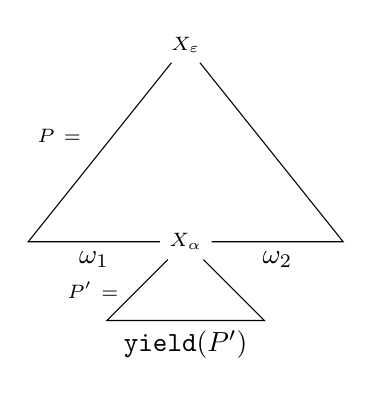
\begin{tikzpicture}
          \node (A) at (0,0) {${\scriptstyle X_\varepsilon}$};
          \coordinate (B) at (-2,-2.5);
          \coordinate (C) at (2,-2.5);
          \node (D) at (0,-2.5) {${\scriptstyle X_\alpha}$};
          \coordinate (E) at (-1,-3.5);
          \coordinate (F) at (1,-3.5);
          
          \draw (A) -- node[above left]{${\scriptstyle P\ =\ }$} (B) -- node[below]{$\omega_1$}(D) -- node[below]{$\omega_2$}(C) -- (A);
          \draw (D) -- node[left]{${\scriptstyle P'\ =\ }$}(E) -- node[below]{$\texttt{yield}(P')$}(F) -- (D);
          
          % \draw [photon] (A) -- node[left]{$\alpha$} (D);
        \end{tikzpicture}
        \caption{$P'' = P \odot P'$}
      \end{subfigure}
      \caption{Конкатенация на дървета}
    \end{figure}
  \end{problem}
  
  Сега да разгледаме частния случай, когато разгледаме $P$ вместо $P'$ в горните условия. Тогава имаме, че $X_\varepsilon = X_\alpha$.
  Дефинираме $n$-тата степен на дървото $P$ по следния начин:
  \begin{itemize}
\item
  $P^{(0)} \df (T_0,\lambda_0)$, където $T_0 = \{\varepsilon\}$ и $\lambda_0(\varepsilon) = \texttt{root}(P)$;
\item
  $P^{(n+1)} \df P^{(n)} \odot P$.
\end{itemize}

\begin{problem}
  Докажете, че $P \odot (P \odot P) = (P \odot P) \odot P$.
\end{problem}


\begin{problem}
  Докажете, че $P^{(n+k)} = P^{(n)} \odot P^{(k)}$.
\end{problem}

\begin{framed}
  \begin{problem}
    \label{prob:tree:iteration}
    Нека $\texttt{yield}(P) = \omega_1 \cdot \texttt{root}(P) \cdot \omega_2$, за някои думи $\omega_1, \omega_2 \in \Sigma^\star$.
    Докажете, че за всяко естествено число $i$ е изпълнено, че:
    \[\texttt{yield}(P^{(i)}) = \omega^i_1 \cdot \texttt{root}(P) \cdot \omega^i_2.\]
  \end{problem}
\end{framed}
\begin{hint}
  Картинката за $i = 2$ изглежда така:

  \begin{figure}[H]
    \begin{subfigure}[t]{0.5\textwidth}
      \centering
      \begin{tikzpicture}
        \coordinate (A) at (0,0);
        \coordinate (B) at (-2,-2.5);
        \coordinate (C) at (2,-2.5);
        \coordinate (D) at (0,-2.5);
        \coordinate (E) at (-2,-5);
        \coordinate (F) at (2,-5);
        \coordinate (G) at (0,-5);
        
        \draw (A) -- node[above left]{$T$} (B) -- (C) -- (A);
        \draw (D) -- node[left]{$T$} (E) -- (F) -- (D);
        
        \draw [photon] (A) -- node[left]{$\alpha$} (D);
        \draw [photon] (D) -- node[left]{$\alpha$} (G);
      \end{tikzpicture}
      \caption{}
    \end{subfigure}
    $\stackrel{\lambda}{\Rightarrow}$
    \begin{subfigure}[t]{0.5\textwidth}
      \centering
      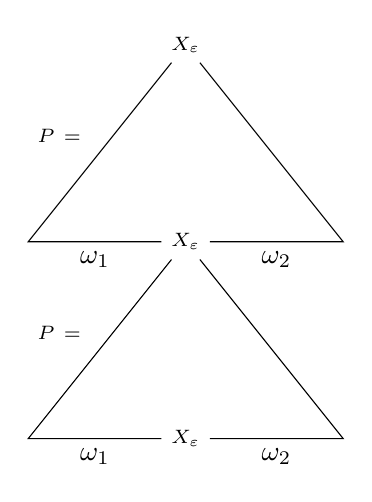
\begin{tikzpicture}
        \node (A) at (0,0) {${\scriptstyle X_\varepsilon}$};
        \coordinate (B) at (-2,-2.5);
        \coordinate (C) at (2,-2.5);
        \node (D) at (0,-2.5) {${\scriptstyle X_\varepsilon}$};
        \coordinate (E) at (-2,-5);
        \coordinate (F) at (2,-5);
        \node (G) at (0,-5) {${\scriptstyle X_\varepsilon}$};
        
        \draw (A) -- node[above left]{${\scriptstyle P\ =\ }$} (B) -- node[below]{$\omega_1$}(D) -- node[below]{$\omega_2$}(C) -- (A);
        \draw (D) -- node[above left]{${\scriptstyle P\ =\ }$}(E) -- node[below]{$\omega_1$} (G) -- node[below]{$\omega_2$} (F) -- (D);
      \end{tikzpicture}
      \caption{$\texttt{yield}(P^{(2)}) = \omega^2_1 \cdot \texttt{root}(P) \cdot \omega^2_2$}
    \end{subfigure}
    \caption{Степенуване на $P$.}
  \end{figure}
\end{hint}

\begin{problem}
  Нека $P = (T,\lambda)$ е дърво на извод съвместимо с граматиката $G$ и нека разгледаме думата $\alpha \in T$.
  % Дефинираме $P \setminus P_\alpha = (T',\lambda')$ по следния начин:
  Дефинираме $\uppercut{P}{\alpha} = (T',\lambda')$ по следния начин:
  \begin{itemize}
  \item
    \mynote{Съобразете, че $\alpha \in \texttt{front}(T')$.}
    $T' = T \setminus \{ \gamma \in T\mid \alpha \prec \gamma\}$, т.е. взимаме същинските разширения на $\alpha$
  \item
    $\lambda'(\gamma) = \lambda(\gamma)$ за $\gamma \in T'$.
  \end{itemize}
  Докажете, че $\uppercut{P}{\alpha}$ е дърво на извод съвместимо с граматиката $G$ и 
  \[P = (\uppercut{P}{\alpha}) \odot (\lowercut{P}{\alpha}).\]
\end{problem}
\begin{hint}
  Имаме следната картинка:

  \begin{figure}[H]
    \begin{subfigure}[t]{0.5\textwidth}
      \centering
      \begin{tikzpicture}
        \coordinate (A) at (0,0);
        \coordinate (B) at (-2,-2.5);
        \coordinate (C) at (2,-2.5);
        \coordinate (D) at (-0.9,-2.5);
        \coordinate (E) at (0.9,-2.5);
        \coordinate (F) at (0,-1.5);
        
        \coordinate (G) at (0,-2.3);
        \coordinate (H) at (-0.9,-3.3);
        \coordinate (I) at (0.9,-3.3);
        
        \draw (A) -- node[above left]{${\scriptstyle T'\ =\ }$}(B) -- (D) -- (F) -- (E) -- (C) -- (A);
        \draw (G) -- node[left]{${\scriptstyle T_\alpha\ =\ }$} (H) -- (I) -- (G);
        
        \draw [photon] (A) -- node[left]{$\alpha$} (F);
      \end{tikzpicture}
      \caption{$T_\alpha = \alpha^{-1}(T)$}
    \end{subfigure}
    $\stackrel{\lambda}{\Rightarrow}$
    \begin{subfigure}[t]{0.5\textwidth}
      \centering
      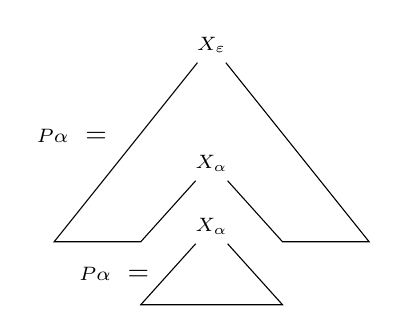
\begin{tikzpicture}
        \node (A) at (0,0) {${\scriptstyle X_\varepsilon}$};
        \coordinate (B) at (-2,-2.5);
        \coordinate (C) at (2,-2.5);
        \coordinate (D) at (-0.9,-2.5);
        \coordinate (E) at (0.9,-2.5);
        \node (F) at (0,-1.5) {${\scriptstyle X_\alpha}$};
        
        \node (G) at (0,-2.3) {${\scriptstyle X_\alpha}$};
        \coordinate (H) at (-0.9,-3.3);
        \coordinate (I) at (0.9,-3.3);
        
        \draw (A) -- node[above left]{${\scriptstyle \uppercut{P}{\alpha}}\ =\ $}(B) -- (D) -- (F) -- (E) -- (C) -- (A);
        \draw (G) -- node[left]{${\scriptstyle \lowercut{P}{\alpha}}\ =\ $} (H) -- (I) -- (G);
      \end{tikzpicture}
      \caption{$\texttt{yield}(\uppercut{P}{\alpha}) = \omega_1 \cdot \texttt{root}(\lowercut{P}{\alpha}) \cdot \omega_2$}
    \end{subfigure}
  \end{figure}
\end{hint}


\subsection*{Най-ляв извод в граматика}
\index{граматика!най-ляв извод}
В нашата дефиниция на извод, изборът върху коя променлива да приложим правило от граматиката е недетерминистичен.
В някои случаи, за нас ще бъде важно винаги да правим детерминистичен избор на това върху коя променлива прилагаме правило.

За две думи $\alpha,\beta \in (V\cup\Sigma)^\star$, дефинираме {\bf най-ляв извод} в граматиката $G$, $\alpha \lderive{\ell} \beta$, по следния начин:
\begin{prooftree}
  \AxiomC{}
  \UnaryInfC{$\alpha \lderive{0} \alpha$}
\end{prooftree}

\begin{prooftree}
  \AxiomC{$A \to_G \gamma$}
  \AxiomC{$\alpha \in \Sigma^\star$}
  \BinaryInfC{$\alpha A \beta \lderive{1} \alpha \gamma \beta$}
\end{prooftree}

\begin{prooftree}
  \AxiomC{$\alpha \lderive{1} \gamma$}
  \AxiomC{$\gamma \lderive{\ell} \beta$}
  \BinaryInfC{$\alpha \lderive{\ell+1} \beta$}
\end{prooftree}

\begin{lemma}
  За всяка безконтекстна граматика $G$, променлива $A \in V$  и дума $\alpha \in (V\cup\Sigma)^\star$,
  \[A \lderive{\star} \alpha\text{ точно тогава, когато } A \derive{\star} \alpha.\]
\end{lemma}
\begin{hint}
  Очевидно е, че ако $A \lderive{\star} \alpha$, то $A \derive{\star} \alpha$.
  За другата посока, достатъчно е да се докаже, че ако $P$ е дърво на извод с корен $A$ и $\texttt{yield}(P) = \alpha$,
  то $A \lderive{\star} \alpha$.

  Индукция по $\texttt{high}(P)$.
\end{hint}



%%% Local Variables:
%%% mode: latex
%%% TeX-master: "../eai"
%%% End:

\section{Извод върху синтактично дърво}

\mynote{Не знам да има учебник, в който формално да е въведена тази релация. Тя е удобна най-вече за решаване на задачи, както и за доказателството на лемата за покачването.}
\begin{definition}
  За произволна безконтекстна граматика $G$, дефинираме релацията $X \yield{\ell} \alpha$, където $X \in V \cup \Sigma$ и $\alpha \in (V\cup\Sigma)^\star$, по следния начин:
  \begin{important}
    \begin{prooftree}
      \AxiomC{}
      \RightLabel{\scriptsize{правило (0)}}
      \UnaryInfC{$X \yield{0} X$}
    \end{prooftree}
    
    \begin{prooftree}
      \AxiomC{$X \to_G X_1\cdots X_n$}
      \AxiomC{$X_1 \yield{\ell_1} \gamma_1$}
      \AxiomC{$\cdots$}
      \AxiomC{$X_n \yield{\ell_n} \gamma_n$}
      \LeftLabel{\scriptsize{($\ell = \sup\{\ell_1,\dots,\ell_n\})$}}
      \RightLabel{\scriptsize{правило (1)}}
      \QuaternaryInfC{$X \yield{\ell+1} \gamma_1\cdots\gamma_n$}
    \end{prooftree}
  \end{important}
\end{definition}

Да напомним, че по дефиниция, ако $n = 0$, то $X_1\cdots X_n = \varepsilon$.
Освен това, понеже $\sup(A)$ означава най-малкото естествено число по-голямо от всички елементи на $A$, то $\sup(\emptyset) = 0$.
Това означава, че ако в граматиката имаме правилото $A \to_G \varepsilon$, то според правило (1)
получаваме, че $A \yield{1} \varepsilon$.

\mynote{ Съобразете, че имаме:
\begin{prooftree}
  \AxiomC{$X \to_G \gamma$}
  \UnaryInfC{$X \yield{1} \gamma$.}
\end{prooftree}
Обърнете внимание също, че тази релация е рефликсивна, но не е транзитивна!}

Да дефинираме $\yield{\star}$ по следния начин:
\[X \yield{\star} \gamma \dff (\exists \ell\in\Nat)[X \yield{\ell} \gamma].\]

Релацията $\yield{\star}$ е удобна, когато не се интересуваме от реда, по който прилагаме правилата за извод в една безконтекстна граматика.

\begin{lemma}
  Нека $G$ е безконтекстна граматика, $X \in V \cup \Sigma$ и $\beta \in (V \cup \Sigma)^\star$.
  Тогава ако $X \derive{\star} \beta$, то $X \yield{\star} \beta$.
\end{lemma}  
\begin{proof}
  С пълна индукция по $\ell$ ще докажем, че ако $X \derive{\ell} \beta$, то $X \yield{\star} \beta$.
  \begin{itemize}
  \item
    $\ell = 0$, т.е. $X \derive{0} X$.
    Тогава е ясно, че $X \yield{\star} X$.
  \item
    Нека $\ell > 0$ и $X \derive{\ell} \beta$.
    Според правилата на извод в граматика имаме извода

    \begin{prooftree}
      \AxiomC{$X \to_G X_1\cdots X_k$}
      \AxiomC{$X_1\cdots X_k \derive{\ell-1} \beta$}
      % \RightLabel{\scriptsize{правило (1)}}
      \BinaryInfC{$X \derive{\ell} \beta$}
    \end{prooftree}

    \mynote{Естествено, че е възможно някои $X_i$ да са букви от $\Sigma$. Тогава $\beta_i = X_i$ и $X_i \derive{0}_G \beta_i$.}
    Щом имаме, че $X_1\cdots X_k \derive{\ell-1} \beta$, от \Proposition{grammar:divide} знаем, че съществува разбиване на $\beta$ на $k+1$ части, така че:
    \begin{itemize}
    \item
      $\beta = \beta_1 \cdots \beta_{k}$;
    \item
      $X_i \derive{\ell_i} \beta_i$, за всяко $i = 1,\dots,k$;
    \item
      $\ell-1 = \sum^k_{i=1} \ell_i$.
    \end{itemize}
    Понеже $\ell_i < \ell$ за всяко $i = 1,\dots,k$, получаваме следното:
    \begin{prooftree}
      \AxiomC{$X \to_G X_1\cdots X_k$}
      \AxiomC{$X_1 \derive{\ell_1} \beta_1$}
      \RightLabel{\scriptsize{\IndHyp}}
      \UnaryInfC{$X_1 \yield{\star} \beta_1$}
      \AxiomC{$\cdots$}
      \AxiomC{$X_k \derive{\ell_k} \beta_k$}
      \RightLabel{\scriptsize{\IndHyp}}
      \UnaryInfC{$X_k \yield{\star} \beta_k$}
      \RightLabel{\scriptsize{правило (1)}}
      \QuaternaryInfC{$X \yield{\star} \underbrace{\beta_1\cdots\beta_k}_{\beta}$}
    \end{prooftree}
  \end{itemize}
\end{proof}

\begin{lemma}
  Нека $G$ е безконтекстна граматика, $X \in V \cup \Sigma$ и $\gamma \in (V \cup \Sigma)^\star$.
  Тогава ако $X \yield{\star} \gamma$, то $X \derive{\star} \gamma$.
\end{lemma}
\begin{proof}
  С пълна индукция по $\ell$ ще докажем, че ако $X \yield{\ell} \gamma$, то $X \derive{\star} \gamma$.
  \begin{itemize}
  \item
    Нека $\ell = 0$. Това означава, че $X \yield{0} X$. Ясно е, че $X \derive{\star} X$.
  \item
    Нека $\ell > 0$. Тогава имаме следното:
    \begin{prooftree}
      \AxiomC{$X \to_G X_1\cdots X_n$}
      \AxiomC{$X_1 \yield{\ell_1} \gamma_1$}
      \AxiomC{$\cdots$}
      \AxiomC{$X_n \yield{\ell_n} \gamma_n$}
      \RightLabel{\scriptsize{($\ell = 1 + \sup\{\ell_1,\dots,\ell_n\})$}}
      \QuaternaryInfC{$X \yield{\ell} \underbrace{\gamma_1\cdots\gamma_n}_{\gamma}$}
    \end{prooftree}
    Понеже $\ell_i < \ell$ за всяко $i = 1,\dots,n$, получаваме следното:
    \begin{prooftree}
      \AxiomC{$X \to_G X_1 \cdots X_{n}$}
      \AxiomC{$X_1 \yield{\ell_1} \gamma_1$}
      \RightLabel{\scriptsize{\IndHyp}}
      \UnaryInfC{$X_1 \derive{\star} \gamma_1$}
      \AxiomC{$\cdots$}
      \AxiomC{$X_n \yield{\ell_n} \gamma_n$}
      \RightLabel{\scriptsize{\IndHyp}}
      \UnaryInfC{$X_n \derive{\star} \gamma_n$}
      \RightLabel{\scriptsize{(\ShortProposition{unrestricted-grammar:concat})}}
      \TrinaryInfC{$X_1 \cdots X_{n} \derive{\star} \gamma_1\cdots\gamma_{n}$}
      % \RightLabel{\scriptsize{правило (1)}}
      \BinaryInfC{$X \derive{\star} \underbrace{\gamma_1\cdots\gamma_{n}}_{\gamma}$}
    \end{prooftree}
  \end{itemize}
\end{proof}

Комбинирайки предишните две леми получаваме следната теорема.
\begin{framed}
  \begin{theorem}\label{th:grammar:yield-derive-equivalent}
    Нека $G$ е безконтекстна граматика, $X \in V \cup \Sigma$ и $\gamma \in (V \cup \Sigma)^\star$.
    Тогава $X \yield{\star} \gamma$ точно тогава, когато $X \derive{\star} \gamma$.
    В частност,
    \[\L(G) = \{\alpha \in \Sigma^\star \mid S \yield{\star}\alpha\}.\]
  \end{theorem}  
\end{framed}

Следващото твърдение ни казва, че има пряка връзка между релацията $\yield{\star}$ и синтактичните дървета.

\begin{important}
  \begin{proposition}\label{pr:yield-relation:parse-tree}
    Нека $G$ е безконтекстна граматика. Тогава
    $X \yield{\ell} \gamma$ точно тогава, когато съществува дърво на извод $P$ съвместимо с $G$, за което
    $\texttt{root}(P) = X$, $\texttt{yield}(P) = \gamma$ и $\texttt{height}(P) = \ell$.
  \end{proposition}
\end{important}
\begin{hint}
  Индукция по $\ell$.
\end{hint}


%%% Local Variables:
%%% mode: latex
%%% TeX-master: "../eai"
%%% End:

\newpage
\subsection{Примерни задачи}

\begin{extra}

Да напомним, че в Раздел~\ref{sect:regular:minimisation} дефинирахме език $\L_\A(q)$.
Сега ще дефинираме език $\L_G(A)$, за произволна променлива $A$.
\[\L_G(A) \df \{\alpha \in \Sigma^\star \mid A \yield{\star}\alpha\}.\]
Ясно е, че $\L(G) = \L_G(S)$.
Също така, да дефинираме апроксимациите $\L^\ell_G(A)$ на $\L_G(A)$ по следния начин:
\[\L^\ell_G(A) \df \{\alpha \in \Sigma^\star \mid A \yield{\leq \ell} \alpha\}.\]
Следните свойства са ясни:
\begin{itemize}
\item
  $\L^0_G(A) = \emptyset$;
\item
  $\L^\ell_G(A)$ е краен език за всяко $\ell$;
\item
  $\L^\ell_G(A) \subseteq \L^{\ell+1}_G(A)$ за всяко $\ell$;
\item
  $\L_G(A) = \bigcup_{\ell\geq 0}\L^\ell_G(A)$.  
\end{itemize}

Следната характеризация на езиците $\L^\ell_G(A)$ ще е удобна за нас, когато искаме да докажем,
че една безконтекстна граматика разпознава даден език.

\begin{proposition}\label{pr:grammar:yield-approximation}
  Нека $G$ е произволна безконтекстна граматика и $A$ е променлива в $G$.
  Тогава имаме следното:
  \begin{align*}
    \L^0_G(A) & = \emptyset\\
    \L^{\ell+1}_G(A) & = \bigcup\{\{\alpha_1\}\cdot \L^\ell_G(A_1) \cdots \{\alpha_n\} \cdot \L^\ell_G(A_n) \cdot \{\alpha_{n+1}\} \mid A \to_G \alpha_1A_1\cdots\alpha_nA_n\alpha_{n+1}\}.
  \end{align*}
\end{proposition}
\begin{proof}
  Пълна индукция по $\ell$. Твърдението очевидно е изпълнено за $\ell = 0$.
  Нека $\alpha \in \L^{\ell+1}_G(A)$, т.е. $A \yield{\leq \ell+1} \alpha$. Имаме следния извод:
  \begin{prooftree}
    \AxiomC{$A \to_G \alpha_1B_1\cdots\alpha_n B_n\alpha_{n+1}$}
    \AxiomC{$B_1 \yield{\leq\ell} \beta_1$}
    \AxiomC{$\cdots$}
    \AxiomC{$B_n \yield{\leq \ell} \beta_n$}
    \QuaternaryInfC{$A \yield{\leq\ell+1} \underbrace{\alpha_1\beta_1\cdots\alpha_n\beta_n\alpha_{n+1}}_{\alpha}$}
  \end{prooftree}
  Понеже $B_i \yield{\leq \ell} \beta_i$, то от \IndHyp имаме, че $\beta_i \in \L^\ell_G(B_i)$.
  Тогава 
  \[\alpha \in \bigcup\{\{\alpha_1\}\cdot \L^\ell_G(A_1) \cdots \{\alpha_n\} \cdot \L^\ell_G(A_n) \cdot \{\alpha_{n+1}\} \mid A \to_G \alpha_1A_1\cdots\alpha_nA_n\alpha_{n+1}\}\]

  Обратно, нека сега $\alpha = \alpha_1\beta_1\cdots\alpha_n\beta_n\alpha_{n+1}$, където $A \to_G \alpha_1B_1\cdots\alpha_nB_n\alpha_{n+1}$,
  $\beta_i \in \L^\ell_G(B_i)$ и $\alpha = \alpha_1\beta_1\cdots\alpha_n\beta_n\alpha_{n+1}$.
  Получаваме следния извод:
  \begin{prooftree}
    \AxiomC{$A \to_G \alpha_1B_1\cdots\alpha_nB_n\alpha_{n+1}$}
    \AxiomC{$\beta_1 \in \L^\ell_G(B_1)$}
    \RightLabel{\scriptsize{\IndHyp}}
    \UnaryInfC{$B_1 \yield{\leq \ell }\beta_1 $}
    \AxiomC{$\cdots$}
    \AxiomC{$\beta_n \in \L^\ell_G(B_n)$}
    \RightLabel{\scriptsize{\IndHyp}}
    \UnaryInfC{$B_n \yield{\leq \ell }\beta_n$}
    \QuaternaryInfC{$A \yield{\leq \ell+1} \underbrace{\alpha_1\beta_1\cdots\alpha_n\beta_n\alpha_{n+1}}_{\alpha}$}
  \end{prooftree}
\end{proof}

\begin{corollary}\label{cor:grammar:yield-approximation}
  Нека $G$ е произволна безконтекстна граматика и $A$ е променлива в $G$. Тогава
  \[\L_G(A) = \bigcup\{\{\alpha_1\}\cdot \L_G(A_1) \cdots \{\alpha_n\} \cdot \L_G(A_n) \cdot \{\alpha_{n+1}\} \mid A \to_G \alpha_1A_1\cdots\alpha_nA_n\alpha_{n+1}\}.\]
\end{corollary}


Като първи пример, нека да видим, че съществува безконтекстен език, който не е регулярен.
Да напомним, че вече видяхме, че езикът $L = \{a^nb^n \mid n\in\Nat\}$ не е регулярен.
\begin{example}\label{ex:grammar:anbn}
  Да разгледаме безконтекстната граматика $G$ зададена със следните правила:
  \begin{align*}
    & S \to aSb \mid \varepsilon.
  \end{align*}
  Тогава
  \begin{align*}
    & \L^0_G(S) = \emptyset\\
    & \L^1_G(S) = \{a\} \cdot \emptyset \cdot \{b\} \cup \{\varepsilon\} = \{\varepsilon\}\\
    & \L^{2}_G(S) = \{a\} \cdot \{\varepsilon\} \cdot \{b\} \cup \{\varepsilon\} = \{\varepsilon, ab\}\\
    & \L^{3}_G(S) = \{a\} \cdot \{\varepsilon, ab\} \cdot \{b\} \cup \{\varepsilon\} = \{\varepsilon,ab,aabb\} = \{a^nb^n \mid n < 3\}\\
    & \vdots
  \end{align*}
  Лесно се съобразява, че
  \[\L^\ell_G(S) = \{a^nb^n \mid n < \ell\}.\]
  Заключаваме, че:
  \[\L(G) = \L_G(S) = \bigcup_{\ell}\L^\ell_G(S) = \{a^nb^n \mid n\in\Nat\}.\]
\end{example}

\begin{example}
  Да разгледаме безконтекстната граматика $G$ зададена със следните правила:
  \begin{align*}
    & S \to aSc\ |\  B\\
    & B \to bBc\ |\ \varepsilon.
  \end{align*}
  Да видим защо $\L(G) = \{a^nb^kc^{n+k} \mid n,k\in\Nat\}$.
  Първо ще докажем \emph{коректност} на граматиката. Това означава, че $G$ не генерира думи извън езика, т.е.
  $\L_G(S) \subseteq \{a^nb^kc^{n+k} \mid n,k\in\Nat\}$. За да направим това обаче, трябва да знаем също така и $\L_G(B)$.
  Формално казано, трябва да докажем, че за всяко $\ell$ е изпълнено следното:
  \begin{align}
    \L^\ell_G(S) & \subseteq \{a^nb^kc^{n+k} \mid n,k\in\Nat\} \label{eq:nknk1}\\
    \L^\ell_G(B) & \subseteq \{b^kc^k \mid k \in \Nat\} \label{eq:nknk2}.
  \end{align}
  Това ще направим с индукция по $\ell$.
  Да напомним, че според \Proposition{grammar:yield-approximation} имаме следните връзки:
  \begin{align*}
    & \L^0_G(S) = \emptyset\\
    & \L^{\ell+1}_G(S) = \{a\} \cdot \L^\ell_G(S) \cdot \{c\} \cup \L^\ell_G(B)\\
    & \L^0_G(B) = \emptyset\\
    & \L^{\ell+1}_G(B) = \{b\} \cdot \L^\ell_G(B) \cdot \{c\} \cup \{\varepsilon\}.
  \end{align*}
  Очевидно е, че \Property{eq:nknk1} и \Property{eq:nknk2} са изпълнени за $\ell = 0$.
  Да примем, че имаме \Property{eq:nknk1} и \Property{eq:nknk2} за някое $\ell$.
  \mynote{Обърнете внимание, че не можем да докажем \Property{eq:nknk1} независимо от \Property{eq:nknk2}.}
  Ще докажем свойствата и за $\ell+1$.
  \begin{itemize}
  \item
    Първо, нека $\alpha \in \L^{\ell+1}_G(S)$. Имаме два случая.
    \begin{itemize}
    \item
      Нека $\alpha \in \{a\} \cdot \L^\ell_G(S) \cdot \{c\}$. От \IndHyp следва, че
      $\alpha = a^{n+1}b^kc^{n+k+1}$ за някои естествени числа $n$ и $k$.
      Тогава е ясно, че $\alpha \in \{a^nb^kc^{n+k} \mid n,k\in\Nat\}$.
    \item
      Нека $\alpha \in  \L^\ell_G(B)$. От \IndHyp следва, че
      $\alpha \in \{b^kc^k \mid k \in \Nat\} \subseteq \{a^nb^kc^{n+k} \mid n,k\in\Nat\}$.
    \end{itemize}
  \item
    Второ, нека $\alpha \in \L^{\ell+1}_G(B)$. Имаме два случая.
    \begin{itemize}
    \item
      Нека $\alpha \in \{b\} \cdot \L^\ell_G(B) \cdot \{c\}$. От \IndHyp следва, че
      $\alpha = b^{k+1}c^{k+1}$ за някое естествено число $k$.
      Тогава е ясно, че $\alpha \in \{b^{k}c^{k} \mid k\in\Nat\}$.
    \item
      Нека $\alpha = \varepsilon$. В този случай също е ясно, че $\alpha \in \{b^{k}c^{k} \mid k\in\Nat\}$.
    \end{itemize}
  \end{itemize}
  Оттук заключаваме, че $\L_G(S) \subseteq \{a^nb^kc^{n+k} \mid n,k\in\Nat\}$.
  
  Сега да разгледаме пълнота на граматиката, което означава, че
  всяка дума от езика се генерира от $G$. С други думи, $\{a^nb^kc^{n+k} \mid n,k\in\Nat\} \subseteq \L_G(S)$.
  Първо ще докажем, че
  \begin{equation}
    \label{eq:4}
      \{b^kc^k \mid k \in \Nat\} \subseteq \L_G(B).
    \end{equation}
    Това ще направим с \emph{пълна} индукция по дължината на думата.
    Да разгледаме произволна дума $\alpha \in \{b^kc^k \mid k \in \Nat\}$.
    \begin{itemize}
    \item
      Нека $|\alpha| = 0$, т.е. $\alpha = \varepsilon$.
      Ясно е, че $\alpha \in \L_G(B)$.
    \item
      Нека $|\alpha| > 0$, т.е. $\alpha = b^{k+1}c^{k+1}$.
      От \IndHyp за \Property{eq:4} следва, че $\alpha \in \{b\} \cdot \L_G(B) \cdot \{c\} \subseteq \L_G(B)$.
    \end{itemize}
    Вече сме готови да докажем, че:
    \begin{equation}
      \label{eq:9}
      \{a^nb^kc^{n+k} \mid n,k \in \Nat\} \subseteq \L_G(S).
    \end{equation}
    Това включване пак ще докажем с \emph{пълна} индукция по дължината на думата.
    Да разгледаме произволна дума $\alpha \in L$. 
    \begin{itemize}
    \item
      Нека $|\alpha| = 0$, т.е. $\alpha = \varepsilon$.
      Ясно е, че $\alpha \in \L_G(B) \subseteq \L_G(S)$.
    \item
      Нека сега $|\alpha| > 0$, т.е. $\alpha = a^nb^kc^{n+k}$, където $n > 0$ или $k > 0$. Да разгледаме два случая.
      \begin{itemize}
      \item
        Нека $n = 0$. Тогава $\alpha = b^kc^k$ и $k > 0$. Тогава от \Property{eq:4}
        следва, че $\alpha \in \L_G(B) \subseteq \L_G(S)$.
      \item                   
        Нека $n > 0$. Тогава от \IndHyp за \Property{eq:9} следва, че
        $\alpha \in \{a\} \cdot \L_G(S) \cdot \{c\} \subseteq \L_G(S)$.
      \end{itemize}
    \end{itemize}
    Доказахме коректност и пълнота на граматиката и следователно $\L(G) = \{a^nb^kc^{n+k} \mid n,k\in\Nat\}$.
  \end{example}
  
  
  \begin{example}
    Нека да видим защо езикът $L = \{a^mb^nc^k\mid m+n \geq k\}$ е безконтекстен.
    Да разгледаме граматиката $G$ с правила
    \begin{align*}
      S& \rightarrow aSc\ |\ aS\ |\ B\\
      B& \rightarrow bBc\ |\  bB\ |\ \varepsilon.
    \end{align*}
    От \Proposition{grammar:yield-approximation} имаме, че:
    \begin{align*}
      \L^0_G(S) & = \emptyset\\
      \L^{\ell+1}_G(S) & = \{a\} \cdot \L^\ell_G(S) \cdot \{c\} \cup \{a\}\cdot \L^\ell_G(S) \cup \L^\ell_G(B)\\
      \L^0_G(B) & = \emptyset\\
      \L^{\ell+1}_G(B) & = \{b\} \cdot \L^\ell_G(B) \cdot \{c\} \cup \{b\} \cdot \L^\ell_G(B) \cup \{\varepsilon\}.
    \end{align*}
    Да предположим, че за произволно естествено число $\ell$ е изпълнено следното:
    \mynote{Тези две свойства ще бъдат нашето \IndHyp. Очевидно е, че те са изпълнени за $\ell = 0$.}
    \begin{align}
      \L^\ell_G(S) & \subseteq \{a^nb^mc^k \mid n+m \geq k\} \\
      \L^\ell_G(B)  & \subseteq \{ b^mc^k \mid m \geq k\}. 
    \end{align}
    Ще докажем, че
    \begin{align*}
      \L^{\ell+1}_G(S) & \subseteq \{a^nb^mc^k \mid n+m \geq k\}\\
      \L^{\ell+1}_G(B)  & \subseteq \{ b^mc^k \mid m \geq k\}.
    \end{align*}
    За първото включване, да разгледаме произволна дума $\alpha \in \L^{\ell+1}_G(S)$. Имаме три случая:
    \begin{itemize}
    \item
      Ако $\alpha \in \L^\ell_G(B)$, то от \IndHyp имаме, че
      \[\alpha \in \{b^mc^k \mid m \geq k\} \subseteq \{a^nb^mc^k \mid n+m \geq k\}.\]
    \item
      Ако $\alpha \in \{a\} \cdot \L^{\ell}_G(S)$, то от \IndHyp имаме, че
      \[\alpha \in \{a^{n+1}b^mc^k \mid n+m \geq k\} \subseteq \{a^nb^mc^k \mid n+m \geq k\}.\]
    \item
      Ако $\alpha \in \{a\} \cdot \L^{\ell}_G(S) \cdot \{c\}$, то от \IndHyp имаме, че
      \[\alpha \in \{a^{n+1}b^mc^{k+1} \mid n+m \geq k\} \subseteq \{a^nb^mc^k \mid n+m \geq k\}.\]
    \end{itemize}
    За второто включване, нека $\alpha \in \L^{\ell+1}_G(B)$. Имаме три случая за думата $\alpha$.
    \begin{itemize}
    \item
      Нека $\alpha \in \{b\} \cdot \L^\ell_G(B) \cdot \{c\}$. Тогава от \IndHyp имаме, че:
      \[\alpha \in \{b^{m+1}c^{k+1} \mid m \geq k\} \subseteq \{b^mc^k \mid  m \geq k\}.\]
    \item
      Нека $\alpha \in \{b\} \cdot \L^\ell_G(B)$. Тогава от \IndHyp имаме, че:
      \[\alpha \in \{b^{m+1}c^{k} \mid m \geq k\} \subseteq \{b^mc^k \mid m \geq k\}.\]
    \item
      Нека $\alpha \in \{\varepsilon\}$. Тогава е ясно, че имаме $\alpha \in \{b^mc^k \mid m \geq k\}$.
    \end{itemize}  
    
    \mynote{Така доказахме \emph{коректност} на граматиката.}
    Заключаваме, че
    \begin{align*}
      \L_G(S) & = \bigcup_\ell\L^\ell_G(S) \subseteq \{a^nb^mc^k \mid n+m \geq k\}\\
      \L_G(B) & = \bigcup_\ell\L^\ell_G(B) \subseteq \{a^nb^mc^k \mid n+m \geq k\}.
    \end{align*}
    
    \mynote{Сега ще докажем \emph{пълнота} на граматиката. Тук ще използваме представянията на $\L_G(S)$ и $\L_G(B)$ според \Corollary{grammar:yield-approximation}.}
    Сега трябва да докажем обратните включвания, а именно:
    \begin{align}
      & \{a^nb^mc^k \mid n+m \geq k\} \subseteq \L_G(S) \label{eq:anbmck:S}\\
      & \{b^mc^k \mid m \geq k\} \subseteq \L_G(B). \label{eq:anbmck:B}
    \end{align}
    
    Трябва да започнем първо със \Property{eq:anbmck:B}.
    Да разгледаме произволна дума $\alpha = b^mc^k$. Трябва да докажем, че $\alpha \in \L_G(B)$.
    Ще направим това с индукция по $m$.
    \begin{itemize}
    \item
      Нека $m = 0$. Това означава, че $\alpha = \varepsilon$. Ясно е, че $\varepsilon \in \L_G(B)$.
    \item
      Нека $m > 0$. Тук имаме два подслучая.
      \begin{itemize}
      \item
        Нека $m = k$. Тогава $\alpha = b \gamma c$ и имаме, че $\gamma = b^{m-1}c^{k-1}$.
        Можем да приложим \IndHyp за $\gamma$ и следователно $\gamma \in \L_G(B)$.
        Получаваме, че $\alpha \in \{b\} \cdot \L_G(B) \cdot \{c\} \subseteq \L_G(B)$.
      \item
        Нека $m > k$. Тогава $\alpha = b \gamma$ и имаме, че $\gamma = b^{m-1}c^k$.
        Можем да приложим \IndHyp за $\gamma$ и следователно $\gamma \in \L_G(B)$.
        Получаваме, че $\alpha \in \{b\} \cdot \L_G(B)\subseteq \L_G(B)$.
      \end{itemize}
    \end{itemize}
    Сега преминаваме към \Property{eq:anbmck:S}.
    Да разгледаме произволна дума $\alpha = a^nb^mc^k$. Трябва да докажем, че $\alpha \in \L_G(S)$.
    Ще направим това с индукция по $n$.
    \begin{itemize}
    \item
      Нека $n = 0$. Тогава $\alpha = b^mc^k$ и $m \geq k$.
      От \Property{eq:anbmck:B} следва, че $\alpha \in \L_G(B) \subseteq \L_G(S)$.
    \item
      Нека $n > 0$. Имаме два подслучая.
      \begin{itemize}
      \item
        Нека $n + m = k$. Тогава $\alpha = a\gamma c$ и $\gamma = a^{n-1}b^mc^{k-1}$.
        Можем да приложим \IndHyp за $\gamma$ и следователно $\gamma \in \L_G(S)$.
        Получаваме, че $\alpha \in \{a\} \cdot \L_G(S) \cdot \{c\} \subseteq \L_G(S)$.
      \item
        Нека $n + m > k$. Тогава $\alpha = a \gamma$ и $\gamma = a^{n-1}b^m c^k$.
        Можем да приложим \IndHyp за $\gamma$ и следователно $\gamma \in \L_G(S)$.
        Получаваме, че $\alpha \in \{a\} \cdot \L_G(S) \subseteq \L_G(S)$.
      \end{itemize}
    \end{itemize}
  \end{example}

\begin{problem}
  Докажете, че езикът $L = \{a^nb^mc^kd^\ell \mid n+k = m + \ell\}$ е безконтекстен.
\end{problem}
\begin{hint}
  Да разгледаме произволна дума от вида $\omega = a^n b^m c^k d^\ell$.
  Имаме два случая.
  \begin{itemize}
  \item
    Ако $n > \ell$, тогава имаме еквивалентността: $\omega \in L \iff (n-\ell) + k = m$.
  \item
    Ако $n \leq \ell$, тогава имаме еквивалентността: $\omega \in L \iff k = m + (\ell- n)$.
  \end{itemize}
  Това наблюдение ни подсказва, че трябва да разгледаме следните езици:
  \begin{align*}
    & L_1 = \{a^nb^mc^k \mid m = n+k\},\\
    & L_2 = \{b^mc^kd^\ell \mid k = m+\ell\}.
  \end{align*}
  Така получаваме, че
  \[L = \{a^n \cdot \omega \cdot d^n \mid n\in\Nat\ \&\ \omega \in L_1 \cup L_2\}.\]
  $L_1$ е безконтекстен език, защото може да се опише с безконтекстната граматика $G_1$ със следните правила:
  \[S_1 \to AC,\quad  A \to aAb\ |\ \varepsilon,\quad C \to bCc\ |\ \varepsilon.\]
  $L_1$ също е безконтекстен език, защото може да се опише с безконтекстната граматика $G_2$ със следните правила:
  \[S_2 \to BD,\quad B \to bBc\ |\ \varepsilon,\quad D \to cCd\ |\ \varepsilon.\]
  Тогава безконтекстната граматика $G$ за $L$ 
  съдържа правилата на граматиките $G_1$ и $G_2$, а също и правилата
  \[S \to aSd\ |\ S_1\ |\ S_2.\]
\end{hint}

\begin{problem}
  \label{prob:equal-but-different}
  \mynote{Ние вече знаем, че този език не е регулярен}
  Докажете, че езикът $L = \{\alpha\beta \in \{a,b\}^\star \mid\ |\alpha| = |\beta|\ \&\ \alpha \neq \beta\}$ е безконтекстен.
\end{problem}
\begin{hint}
  Да разгледаме една произволна дума $\omega$, където $\omega = \alpha\beta$, $|\alpha| = |\beta|$ и $\alpha \neq \beta$.
  Знаем, че същестува индекс $i < |\alpha|$, такъв че думата $\omega$ може да се представи така:
  \[\omega = \alpha\slice{:i} \cdot \alpha\slice{i} \cdot \alpha\slice{i+1:} \cdot \beta\slice{:i} \cdot \beta\slice{i} \cdot \beta\slice{i+1:},\]
  където $\alpha\slice{i} \neq \beta\slice{i}$.

  Нека $n = |\alpha| = |\beta|$ и да представим $n$ като $n = i+1+k$. Имаме два случая.
  \begin{itemize}
  \item
    Ако $k \geq i$, то можем да преставим $\omega$ по следния начин:
    \[\omega = \underbrace{\alpha\slice{:i}}_{\text{дълж. }i} \cdot \alpha\slice{i} \cdot \underbrace{\alpha\slice{i+1:2i+1}}_{\text{дълж. }i} \cdot \underbrace{\alpha\slice{2i+1:} \cdot \beta\slice{:i}}_{\text{дълж. }k} \cdot \beta\slice{i} \cdot \underbrace{\beta\slice{i+1:}}_{\text{дълж. }k}.\]
  \item
    Нека $k < i$, то можем да преставим $\omega$ по следния начин:
    \[\omega = \underbrace{\alpha\slice{:i}}_{\text{дълж. }i} \cdot \alpha\slice{i} \cdot \underbrace{\alpha\slice{i+1:} \cdot \beta\slice{:i-k}}_{\text{дълж. }i} \cdot \underbrace{\beta\slice{i-k:i}}_{\text{дълж. }k} \cdot \beta\slice{i} \cdot \underbrace{\beta\slice{i+1:}}_{\text{дълж. }k}.\]
  \end{itemize}
  От тези представяния на $\omega$ е ясно, че можем да изразим езика $L$ по следния начин:
  \[L = L_a \cdot L_b \cup L_b \cdot L_a,\]
  където:
  \begin{align*}
    & L_a = \{\alpha a \beta \mid \alpha,\beta \in \{a,b\}^\star\ \&\ |\alpha| = |\beta|\}\\
    & L_b = \{\alpha b \beta \mid \alpha,\beta \in \{a,b\}^\star\ \&\ |\alpha| = |\beta|\}.
  \end{align*}
  Сега разгледайте безконтекстната граматика $G$ със следните правила:
  \begin{align*}
    & S \to AB\ |\ BA\\
    & A \to XAX\ |\ a\\
    & B \to XBX\ |\ b\\
    & X \to a\ |\ b.
  \end{align*}
  Лесно се съобразява, че:
  \begin{align*}
    & L_a = \L_G(A)\\
    & L_b = \L_G(B)\\
    & L = \L_G(S).
  \end{align*}
\end{hint}

\begin{problem}
 Докажете, че езикът $L = \{\alpha \sharp \beta \mid \alpha,\beta \in \{a,b\}^\star\ \&\ \alpha \neq \beta \}$ е безконтекстен.
\end{problem}
\begin{hint}
  Разгледайте граматиката:
  \begin{align*}
    & S \to AaR\ |\ BbR\ |\ E\\
    & A \to XAX\ |\ bR\sharp\\
    & B \to XBX\ |\ aR\sharp\\
    & E \to XEX\ |\ XR\sharp\ |\ \sharp XR\\
    & R \to XR\ |\ \varepsilon\\
    & X \to a\ |\ b.
  \end{align*}
  Имаме, че за произволни думи $\alpha,\beta,\gamma,\delta \in \{a,b\}^\star$,
  \begin{align*}
    & S \derive{\star} \alpha b \gamma \sharp \beta a \delta\ \&\ |\alpha| = |\beta|,\\
    & S \derive{\star} \alpha a \gamma \sharp \beta b \delta\ \&\ |\alpha| = |\beta|, \text{ или}\\
    & S \derive{\star} \alpha \sharp \beta\ \&\ |\alpha| \neq |\beta|.
  \end{align*}      
\end{hint}

\begin{problem}
  Докажете, че езикът $L = \{a^nb^mc^kd^\ell \mid n+k \geq m + \ell\}$ е безконтекстен.
\end{problem}

\begin{problem}
  \mynote{
    $S \to aS \mid aSc \mid aB \mid bB$\\
    $B \to bB \mid bBc \mid \varepsilon$
  }
  Докажете, че езикът $L = \{a^mb^nc^k\mid m+n \geq k + 1\}$ е безконтекстен.  
\end{problem}

\begin{problem}
  Докажете, че езикът $L = \{\alpha \sharp \beta \mid \alpha,\beta \in \{a,b\}^\star\ \&\ |\alpha| \neq |\beta| \}$ е безконтекстен.
\end{problem}

\begin{problem}
  Да разгледаме граматиката $G$ с правила
  \[S \to AA\ |\ B,\ A \to B\ |\ bb,\ B \to aa\ |\ aB.\]
  Да се намери езика на тази граматика и да се докаже, че граматиката разпознава точно този език.
\end{problem}

\end{extra}

%%% Local Variables:
%%% mode: latex
%%% TeX-master: "../eai"
%%% End:

\newpage
\section{Лема за покачването}

В този раздел ще разгледаме едно твърдение, което ще ни даде критерий за проверка кога един език не е безконтекстен. Ще започнем с няколко помощни твърдения.

\begin{proposition}\label{pr:pumping:ground}
  За произволни променливи $A$, $B$ и думи $\alpha_1,\alpha_2, \alpha_3$ е изпълнено:
  \begin{prooftree}
    \AxiomC{$A \yield{\ell_1}\alpha_1B\alpha_3$}
    \AxiomC{$B \yield{\ell_2} \alpha_2$}
    \BinaryInfC{$A \yield{ \leq \ell_1+\ell_2} \alpha_1\alpha_2\alpha_3$}
  \end{prooftree}
\end{proposition}
\begin{hint}
  Формално доказателството протича с индукция по $\ell_1$.
  
  \begin{figure}[H]
    \begin{subfigure}[t]{0.5\textwidth}
      \centering
      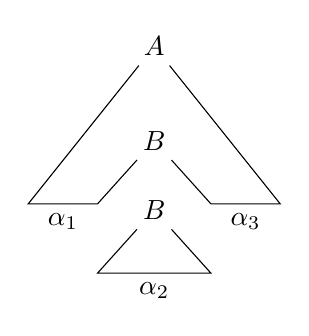
\begin{tikzpicture}[scale=0.8]
        \node (A) at (0,0) {$A$};
        \coordinate (B) at (-2,-2.5);
        \coordinate (C) at (2,-2.5);
        \coordinate (D) at (-0.9,-2.5);
        \coordinate (E) at (0.9,-2.5);
        \node (F) at (0,-1.5) {$B$};
        
        \node (G) at (0,-2.6) {$B$};
        \coordinate (H) at (-0.9,-3.6);
        \coordinate (I) at (0.9,-3.6);
        
        \draw (A) -- (B) -- node[below]{$\alpha_1$} (D) -- (F) -- (E) -- node[below]{$\alpha_3$} (C) -- (A);
        \draw (G) -- (H) -- node[below]{$\alpha_2$}(I) -- (G);
        
        % \draw [photon] (A) -- node[left]{$\alpha$} (F);
      \end{tikzpicture}
      \caption{\scriptsize{Синтактични дървета за изводите $A \yield{\ell_1}\alpha_1B\alpha_3$ и $B \yield{\ell_2} \alpha_2$}}
    \end{subfigure}
    % $\stackrel{\lambda}{\Rightarrow}$
    ~
    \begin{subfigure}[t]{0.5\textwidth}
      \centering
      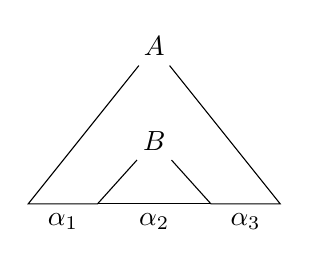
\begin{tikzpicture}[scale=0.8]
        \node (A) at (0,0) {$A$};
        \coordinate (B) at (-2,-2.5);
        \coordinate (C) at (2,-2.5);
        \coordinate (D) at (-0.9,-2.5);
        \coordinate (E) at (0.9,-2.5);
        \node (F) at (0,-1.5) {$B$};
        
        % \coordinate (G) at (0,-2.3) {${\scriptstyle X_\alpha}$};
        % \coordinate (H) at (-0.9,-3.3);
        % \coordinate (I) at (0.9,-3.3);
        
        \draw (A) -- (B) -- node[below]{$\alpha_1$} (D) -- (F) -- (E) -- node[below]{$\alpha_3$} (C) -- (A);
        \draw (D) -- node[below]{$\alpha_2$} (E);
      \end{tikzpicture}
      \caption{\scriptsize{Съединяваме двете дървета}}
      % \caption{$\texttt{yield}(\uppercut{P}{\alpha}) = \omega_1 \cdot \texttt{root}(\lowercut{P}{\alpha}) \cdot \omega_2$}
    \end{subfigure}
  \end{figure}
\end{hint}

\begin{proposition}\label{pr:pumping:iteration}
  За произволна променлива $A$ и произволни думи $\beta$ и $\gamma$ е изпълнено:
  \begin{prooftree}
    \AxiomC{$A \yield{\ell} \beta A \gamma$}
    \AxiomC{$i \in \Nat$}
    \BinaryInfC{$A \yield{\leq i \cdot \ell} \beta^i A \gamma^i$}
  \end{prooftree}
\end{proposition}
\begin{hint}
  Формално доказателството трябва да следва индукция по $i$.
  Понеже това доказателство не крие изненади, ще се задоволим с един пример. Нека $P$ да бъде синтактично дърво съответстващо на извода $A \yield{\ell} \beta A \gamma$.
  Тогава можем да получим синтактично дърво $P^{(2)}$  съответстващо на $A \yield{\leq 2\ell} \beta^2A\gamma^2$ по следния начин.
  \begin{figure}[H]
    \begin{subfigure}[t]{0.3\textwidth}
      \centering
      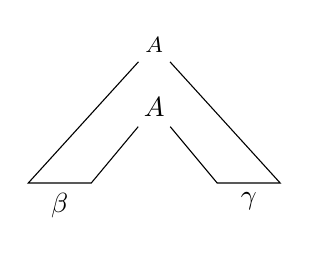
\begin{tikzpicture}[scale=0.8]
        \node (A) at (0,0) {\footnotesize{$A$}};
        \coordinate (B) at (-2,-2.2);
        \coordinate (C) at (2,-2.2);
        \coordinate (S) at (-1,-2.2);
        \coordinate (T) at (1,-2.2);
        \node (L) at (0,-1) {$A$};
        
        \draw (A) -- (B) -- node[below]{$\beta$}(S) -- (L) -- (T) -- node[below]{$\gamma$}(C) -- (A);
      \end{tikzpicture}
      \caption{\scriptsize{Синтактично дърво $P$ за извода $A \yield{\ell} \beta A\gamma$}}
    \end{subfigure}
    ~
    \begin{subfigure}[t]{0.3\textwidth}
      \centering
      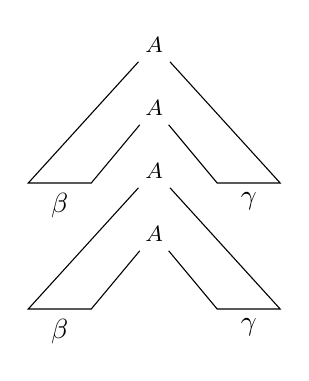
\begin{tikzpicture}[scale=0.8]
        \node       (A) at (0,0) {\footnotesize{$A$}};
        \coordinate (B) at (-2,-2.2);
        \coordinate (C) at (2,-2.2);
        \coordinate (S) at (-1,-2.2);
        \coordinate (T) at (1,-2.2);
        \node       (L) at (0,-1) {\footnotesize{$A$}};
        
        \coordinate (E) at (-0.7,-2.5);
        \coordinate (F) at (0.7,-2.5);
        
        
        \node       (H) at (0,-2) {\footnotesize{$A$}};
        \node       (X) at (0,-3) {\footnotesize{$A$}};
        \coordinate (D) at (-2,-4.2);
        \coordinate (G) at (2,-4.2);
        \coordinate (E) at (-1,-4.2);
        \coordinate (F) at (1,-4.2);
        
        \draw (A) -- (B) -- node[below]{$\beta$}(S) -- (L) -- (T) -- node[below]{$\gamma$}(C) -- (A);
        \draw (H) -- (D) -- node[below]{$\beta$}(E) -- (X) -- (F) -- node[below]{$\gamma$}(G) -- (H);
      \end{tikzpicture}
      \caption{\scriptsize{Съединяваме две копия на $P$}}
    \end{subfigure}
    ~
    \begin{subfigure}[t]{0.3\textwidth}
      \centering
      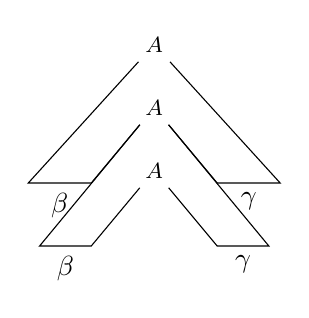
\begin{tikzpicture}[scale=0.8]
        \node       (A) at (0,0) {\footnotesize{$A$}};
        \coordinate (B) at (-2,-2.2);
        \coordinate (C) at (2,-2.2);
        \coordinate (S) at (-1,-2.2);
        \coordinate (T) at (1,-2.2);
        \node       (L) at (0,-1) {\footnotesize{$A$}};
        
        \coordinate (E) at (-0.7,-2.2);
        \coordinate (F) at (0.7,-2.2);
        
        \node       (X) at (0,-2) {\footnotesize{$A$}};
        \coordinate (D) at (-1.82,-3.2);
        \coordinate (G) at (1.82,-3.2);
        \coordinate (E) at (-1,-3.2);
        \coordinate (F) at (1,-3.2);
        
        \draw (A) -- (B) -- node[below]{$\beta$}(S) -- (L) -- (T) -- node[below]{$\gamma$}(C) -- (A);
        \draw (L) -- (D) -- node[below]{$\beta$}(E) -- (X) -- (F) -- node[below]{$\gamma$}(G) -- (L);
      \end{tikzpicture}
      \caption{\scriptsize{Получаваме синтактично дърво $P^{(2)}$ за извода $A \yield{\leq 2\ell} \beta^2 A \gamma^2$}}
    \end{subfigure}
  \end{figure}
\end{hint}

\begin{proposition}\label{pr:pumping:lower-bound}
  Нека $G$ е безконтекстна граматика и 
  \mynote{Числото $b$ е максималната разклоненост, която можем да получим за синтактично дърво на извод в граматикта $G$.}
  \[b \df \max\{\ |\gamma| \mid A \to \gamma \text{ е правило в }G\ \}.\]
  Тогава:
  \begin{itemize}
  \item 
    Ако $A \yield{\leq\ell} \alpha$, то $|\alpha| \leq b^\ell$.
  \item
    Ако $\alpha \in \L(G)$ и $|\alpha| > b^\ell$, то $S \yield{\geq \ell+1} \alpha$.
  \end{itemize}
\end{proposition}

\begin{proof}

%   \begin{proposition}
%   \label{cor:tree:upper-bound}
%   \mynote{Това следствие ще бъде важно за нас, когато разгледаме лемата за покачването за безконтекстни езици.}
%   Нека $P = (T,\lambda)$ е дърво на извод съвместимо с $G$. Тогава
%   \[|\texttt{yield}(P)| \leq b^{{\high}(P)}.\]
% \end{proposition}
% \begin{proof}
%   Следва директно от горното твърдение след като съобразим, че
%   \[|\texttt{yield}(P)| \leq |\leaves(P)|.\]
% \end{proof}

  
  Това твърдение е на практика следствие от \Problem{tree:leaves-upper-bound} в комбинация с \Proposition{yield-relation:parse-tree}.
  \begin{itemize}
  \item
    Да разгледаме синтактично дърво $P = (T,\lambda)$ за извода $A \yield{\leq\ell} \alpha$.
    Според \Problem{tree:leaves-upper-bound} имаме, че $\abs{\alpha} = \abs{\leaves(T)}\leq b^{\high(T)} = b^{\ell}$.
  \item
    Нека $\alpha \in \L(G)$ и $\abs{\alpha} > b^\ell$. Това означава, че $S \yield{\star} \alpha$.
    Ако допуснем, че $S \yield{\leq \ell} \alpha$, то бихме имали, че $\abs{\alpha} \leq b^\ell$, което е противоречие.
    Заключаваме, че $S \yield{\geq \ell+1} \alpha$.
  \end{itemize}
\end{proof}

\begin{important}
  \begin{lemma}[за покачването (безконтекстни езици)]
    \index{лема за покачването!безконтекстни езици}
    \label{lem:context-free:pumping} 
    \mynote{\cite[стр. 125]{sipser3}, \cite[стр. 125]{hopcroft1}, \cite[стр. 275]{hopcroft2}, \cite[стр. 148]{kozen}.}
    За всеки безконтекстен език $L$ съществува $p>0$, такова
    че ако $\alpha\in L$, за която $\abs{\alpha} \geq p$, то съществува разбиване на думата на пет части, $\alpha=xyuvw$,
    \mynote{Ще казваме, че $p$ е константа на покачването. Тук отново да напомним, че $0 \in \Nat$ и $xy^0uv^0w = xuw$.}
    за което е изпълнено:
    \begin{enumerate}[1)]
    \item
      $\abs{yv}\geq 1$,
    \item
      $\abs{yuv}\leq p$, и
    \item
      $(\forall i\in\Nat)[xy^iuv^iw\in L]$.
    \end{enumerate}
  \end{lemma}
\end{important}
\begin{proof}
  \mynote{Числото $b$ е максималната разклоненост на всяко дърво на извод за дума изводима от граматиката $G$.}
  Нека $G$ е безконтекстна граматика за езика $L$. Да положим
  \[p \df b^{\abs{V}+1}, \text{ където }b \df \max\{\ |\gamma| \mid A \to \gamma \text{ е правило в }G\ \}.\]
  Ще покажем, че този избор на $p$ е удачен за удовлетворяването на условията на лемата. Ще наричаме $p$ константа на покачването за граматиката $G$.
  \mynote{Важното е да вземем дума $\alpha \in \L(G)$, за която $\abs{\alpha} > b^{\abs{V}}$.}
  Да разгледаме произволна дума $\alpha \in \L(G)$, за която $\abs{\alpha} \geq p$.
  Понеже $\L(G)$ е безкраен език, то със сигурност можем да намерим такава дума.
  Щом $S \yield{\star} \alpha$, според \Proposition{pumping:lower-bound}, винаги имаме $S \yield{\ell}\alpha$ за $\ell \geq \abs{V}+1$.
  Нека измежду всички синтактични дървета $P = (T,\lambda)$ за извода $S \yield{\ell} \alpha$ сме избрали такова с \emph{минимален} брой елементи в $T$.
  Да фиксираме \emph{максимален} път $\pi$ в $T$, т.е. дума $\pi \in T$ и $|\pi| = \ell$.
  Чрез функцията $\lambda$ пътя $\pi$ определя редицата $X_0,X_1,\dots,X_\ell$, като $X_i = \lambda(\rho)$, където $\rho \prec \pi$ и $\abs{\rho} = i$. Ясно е, че $X_i \in V$ за $i < \ell$ и $X_\ell \in \Sigma \cup \{\varepsilon\}$.
  Щом $\ell \geq \abs{V}+1$, то това означава, че по този път $\pi$
  \mynote{Принципът на Дирихле е известен също и като принципа на чекмеджетата.}
  се срещат $\ell \geq \abs{V}+1$ на брой променливи. От принципа на Дирихле следва, че трябва да има повторения на променливи по този път. 
  Във вече фиксираното синтактично дърво $P$ можем да изберем това срещане на двойка повтарящи се променливи по пътя $\pi$, както на \Figure{pumping:partition}, което е възможно най-близо до края на пътя.
  Това означава, че можем да разбием извода $S \yield{\ell} \alpha$ като $S \yield{\star} xAw$ и $A \yield{\leq \abs{V}+1} \gamma$, където $\alpha = x\gamma w$.
  Сега според нашия избор, изводът $A \yield{\leq \abs{V}+1} \gamma$ може да се разбие като $A \yield{\leq \abs{V}+1} yAv$ и $A \yield{\leq \abs{V}} u$,
  където $\gamma = yuv$.
  Да обобщим. Можем да разбием думата $\alpha$ на пет части като $\alpha = xyuvw$ с изводите:
  \begin{enumerate}[(1)]
  \item
    $S \yield{\star} x A w$, 
  \item
    $A \yield{\leq \abs{V}+1} y u v$, защото в дървото $P$ можем да изберем първата двойка повтарящи се променливи, които срещнем отзад напред по пътя $\pi$. Тук сме означили тази повтаряща се променлива с $А$.
  \item
    $A \yield{\leq \abs{V}} u$, като тук вече няма повтарящи се променливи по останалата част от пътя $\pi$.
  \end{enumerate}

  \begin{figure}[H]
    \begin{subfigure}[t]{0.3\textwidth}
    \centering
    \begin{tikzpicture}[scale=0.8]
      \node (A) at (0,0) {\footnotesize{$S$}};
      \coordinate (B) at (-2,-3);
      \coordinate (C) at (2,-3);
      \node (D) at (0,-1.2) {\footnotesize{$A$}};
      \coordinate (D1) at (1.4,-3);
      \coordinate (D2) at (-1.4,-3);
      \node (E) at (0,-2.3) {\footnotesize{$A$}};
      \coordinate (E1) at (0.7,-3);
      \coordinate (E2) at (-0.7,-3);
      \coordinate (F) at (0,-3);

      \draw (A) -- node[above left]{$P = $} (B) -- node[below]{$\pi$}(C) -- (A);
      \draw [photon2] (A) -- (D) -- (E) -- (F);
    \end{tikzpicture}
    \caption{Първата двойка повтарящи се променливи, които намерим като тръгнем отдолу нагоре по пътя $\pi$.}
    \label{fig:pumping:partition}
  \end{subfigure}
  ~
  \begin{subfigure}[t]{0.3\textwidth}
    \centering
    \begin{tikzpicture}[scale=0.8]
      \node (A) at (0,0) {\footnotesize{$S$}};
      \coordinate (B) at (-2,-3);
      \coordinate (C) at (2,-3);
      \node (D) at (0,-1.2) {\footnotesize{$A$}};
      \coordinate (D1) at (1.4,-3);
      \coordinate (D2) at (-1.4,-3);
      \node (E) at (0,-2.3) {\footnotesize{$A$}};
      \coordinate (E1) at (0.5,-3);
      \coordinate (E2) at (-0.5,-3);
      \coordinate (F) at (0,-3);

      \draw (A) -- node[above left]{$P = $} (B) -- node[below] {$x$} (D2) -- (D) -- (D1) -- node[below]{$w$} (C) -- (A);
      \draw (D2) -- node[below]{$y$} (E2) -- (E) -- (E1) -- node[below]{$v$} (D1);
      \draw (E2) -- node[below]{$u$} (E1);

      \draw [photon2] (A) -- (D) -- (E) -- (F);
    \end{tikzpicture}
    \caption{Разбиваме дървото на три части.}
    \end{subfigure}
    ~
    \begin{subfigure}[t]{0.3\textwidth}
      \centering
      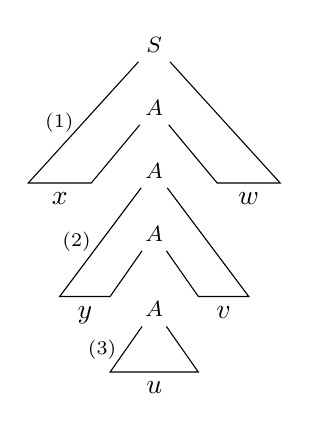
\begin{tikzpicture}[scale=0.8]
        \node (A) at (0,0) {\footnotesize{$S$}};
        \coordinate (B) at (-2,-2.2);
        \coordinate (C) at (2,-2.2);
        \coordinate (S) at (-1,-2.2);
        \coordinate (T) at (1,-2.2);
        \node (L) at (0,-1) {\footnotesize{$A$}};
        
        \coordinate (E) at (-0.7,-2.5);
        \coordinate (F) at (0.7,-2.5);
        
        
        \node (H) at (0,-2) {\footnotesize{$A$}};
        \node (X) at (0,-3) {\footnotesize{$A$}};
        \coordinate (D) at (-1.5,-4);
        \coordinate (G) at (1.5,-4);
        \coordinate (E) at (-0.7,-4);
        \coordinate (F) at (0.7,-4);
        
        \node (I) at (0,-4.2) {\footnotesize{$A$}};
        \coordinate (U) at (-0.7,-5.2);
        \coordinate (V) at (0.7,-5.2);
        
        \draw (A) -- node[left]{\scriptsize{(1)}}(B) -- node[below]{$x$}(S) -- (L) -- (T) -- node[below]{$w$}(C) -- (A);
        \draw (H) -- node[left]{\scriptsize{(2)}}(D) -- node[below]{$y$}(E) -- (X) -- (F) -- node[below]{$v$}(G) -- (H);
        \draw (I) -- node[left]{\scriptsize{(3)}}(U) -- node[below]{$u$}(V) -- (I);
      \end{tikzpicture}
      \caption{Получаваме три отделни синтактични дървета.}
    \end{subfigure}
  \end{figure}
  Сега остава да проверим условието на лемата:
  \begin{itemize}
  \item
    Да допуснем, че $\abs{yv} = 0$. Това означава, че $\alpha = xuw$ и имаме извода:
    \begin{prooftree}
      \AxiomC{$S \yield{\star} xAw$}
      \AxiomC{$A \yield{\star} u$}
      \RightLabel{\scriptsize{(\Proposition{pumping:ground})}}
      \BinaryInfC{$S \yield{\star} \underbrace{xuw}_{\alpha}$,}
    \end{prooftree}
    за който съществува дърво на извод с по-малко на брой възли отколкото $P$, защото махаме средната част, която съдържа поне един възел.
    Това е противоречие с избора на $P$ като синтактично дърво за $S \yield{\star}\alpha$ с минимален брой възли.
    Заключаваме, че $\abs{yv} \geq 1$.
  \item
    Понеже имаме извода $A \yield{\leq\abs{V}+1} yuv$, то от \Proposition{pumping:lower-bound} следва, че $\abs{yuv} \leq b^{\abs{V}+1} = p$.
  \item
    За произволно $i\in\Nat$ имаме извода:
    \begin{prooftree}
      \AxiomC{$A \yield{\star}yAv$}
      \LeftLabel{\scriptsize{(\ShortProposition{pumping:iteration})}}
      \UnaryInfC{$A \yield{\star}y^iAv^i$}
      \AxiomC{$A \yield{\star} u$}
      \LeftLabel{\scriptsize{(\ShortProposition{pumping:ground})}}
      \BinaryInfC{$A \yield{\star} y^iuv^i$}
      \AxiomC{$S \yield{\star}xAw$}
      \LeftLabel{\scriptsize{(\ShortProposition{pumping:ground})}}
      \BinaryInfC{$S \yield{\star} xy^iuv^iw$}
    \end{prooftree}
    Оттук заключаваме, че $(\forall i \in \Nat)[xy^iuv^iw \in \L(G)]$.
  \end{itemize}
\end{proof}

\mynote{\cite[стр. 153]{kozen}.}
Както и при \hyperref[lem:regular:pumping]{Лема за покачването за регулярни езици}, ние ще използваме \emph{контрапозицията} на условието на \hyperref[lem:context-free:pumping]{Лема за покачването за безконтекстни езици} при проверка, че даден език не е безконтекстен.

\begin{corollary}
  \label{cor:pumping-context-free}
  \mynote{Ако $L$ е краен език, то е ясно, че $L$ е безконтекстен.}
  Нека $L$ е произволен {\bf безкраен} език. Нека също така е изпълнено, че:
  \begin{description}
  \item[($\forall$)]
    за {\em всяко} естествено число $p \geq 1$,
  \item[($\exists$)]
    можем да намерим дума $\alpha \in L$, $\abs{\alpha}\geq p$, такава че
  \item[($\forall$)]
    за {\em всяко} разбиване на думата на пет части, $\alpha = xyuvw$, със свойствата $\abs{yv} \geq 1$ и $\abs{yuv} \leq p$,
  \item[($\exists$)]
    можем да намерим $i \in \Nat$, за което е изпълнено, че $xy^iuv^iw \not\in L$.
  \end{description}  
  \mynote{\writedown Докажете! Аналогично е на \Corollary{regular:pumping}}
  Тогава $L$ {\bf не} е безконтекстен език.
\end{corollary}

\begin{corollary}
  \mynote{\writedown Докажете!}
  Нека $G$ е безконтекстна граматика и $p$ е константата на покачването за $G$.
  Тогава $\abs{\L(G)} = \infty$ точно тогава, когато съществува $\alpha \in \L(G)$, за която $p \leq \abs{\alpha} < 2p$.
\end{corollary}
% \begin{proof}
%   Ако съществува дума $\alpha \in L$, за която $\abs{\alpha} \geq p$, то от \Lem{pumping-context} следва,
%   че $\abs{L} = \infty$, защото $\alpha = xyuvw$ и $xy^iuv^iw \in L$, за всяко $i\in\Nat$.

%   За другата посока, нека сега $\abs{L} = \infty$.
%   Да изберем най-късата дума $\alpha \in L$, за която $\abs{\alpha} \geq p$.
%   Ще докажем, че $p \leq \abs{\alpha} < 2p$. За целта да допуснем, че $\abs{\alpha} \geq 2p$.
%   Тогава от \Lem{pumping-context} следва, че $\alpha = xyuvw$, $\abs{yv} \geq 1$, $\abs{yuv} \leq p$, $xy^0uv^0w = xuw \in L$.
%   Ако $\abs{xuw} < p$, то $\abs{yv} > p$, защото $\abs{yv} + \abs{xuw} = \abs{\alpha} \geq 2p$, и следователно $\abs{yuv} > p$, което е противоречие.
%   Следва, че $\abs{\alpha} > \abs{xuw} \geq p$.
%   Получихме, че думата $xuw\in L$ и $\abs{xuw} \geq p$. Това е противоречие с минималността на $\alpha$.
% \end{proof}

% \begin{framed}
%   \Lem{pumping-context} е полезна, когато искаме да докажем, че даден език $L$ {\bf не} е безконтекстен.
%   За целта, доказваме отрицанието на свойствата от \Lem{pumping-context} за $L$, т.е.
%   за всяка константа $p$, ние намираме дума $\alpha \in L$, $\abs{\alpha}\geq p$, такава че за всяко разбиване на думата на пет части, $\alpha = xyuvw$,
%   със свойствата $\abs{yv} \geq 1$ и $\abs{yuv} \leq p$, е изпълнено, че $(\exists i)[xy^iuv^iw \not\in L]$.
% \end{framed}

\begin{remark}
  \mynote{\todo Защо?}
  Алгоритъм за проверка дали един безконтекстен език е безкраен следвайки горния критерий би 
  имал експоненциална сложност относно $|G|$.
\end{remark}

\begin{example}
  \label{ex:context-free:pumping:anbncn}
  Да видим защо езикът $L = \{a^nb^nc^n\ \mid\ n\in\Nat\}$ не е безконтекстен.
  \begin{description}
  \item[$(\forall)$]
    Разглеждаме произволна константа $p \geq 1$.
  \item[$(\exists)$]
    Избираме дума $\alpha \in L$, $\abs{\alpha} \geq p$.
    В случая, нека $\alpha = a^pb^pc^p$.
  \item[$(\forall)$]
    Разглеждаме произволно разбиване на $\alpha$ на пет части $\alpha = xyuvw$, за което $\abs{yuv} \leq p$ и $1 \leq \abs{yv}$.
  \item[$(\exists)$]
    \mynote{\writedown Съобразете, че може да изберете и $i = 0$. В този пример може да вземете едно и също $i$ за всяко разбиване на думата $\alpha$ от предишната стъпка. В други примери ще видим, че изборът на $i$ зависи от разглежданото разбиване на думата.}
    За всяко такова разбиване ще посочим $i$, за което $xy^iuv^iw \not\in L$.
    Знаем, че поне едно от $y$ и $v$ не е празната дума.
    Имаме няколко случая за $y$ и $v$.
    \begin{itemize}
    \item
      $y$ и $v$ са думи съставени от една буква.
      В този случай получаваме, че $xy^2uv^2w$ има различен брой букви $a$, $b$ и $c$.
    \item
      $y$ или $v$ е съставена от две букви.
      В този случай получаваме, че в $xy^2uv^2w$ редът на буквите е нарушен.
    \item
      понеже $\abs{yuv} \leq p$, то не е възможно в $y$ или $v$ да се срещат и трите букви.
    \end{itemize}  
    Оказа се, че във всички възможни случаи за $y$ и $v$, 
    $xy^2uv^2w \not\in L$.
  \end{description}
  Така от \Corollary{pumping-context-free} следва, че езикът $L$ не е безконтекстен.
\end{example}

\begin{framed}
  \begin{proposition}\label{pr:context-free:pumping:non-closure}
    Безконтекстните езици {\bf не} са затворени относно операциите сечение и допълнение.
  \end{proposition}
\end{framed}
\begin{hint}
  Да разгледаме езика $L_0 = \{a^nb^nc^n\mid n\in\Nat\}$, за който вече знаем от \Example{context-free:pumping:anbncn}, че не е безконтекстен.
  Да вземем също така и безконтекстните езици 
  \mynote{\writedown Защо $L_1$ и $L_2$ са безконтекстни?}
  \[L_1 = \{a^nb^nc^m\mid n,m\in\Nat\},\ L_2 = \{a^mb^nc^n\mid n,m\in\Nat\}.\]
  \mynote{Да напомним, че с $\ov{L}$ означаваме допълнението на езика $L$, т.е. $\ov{L} \df \Sigma^\star \setminus L$.}
  \begin{itemize}
  \item 
    Понеже $L_0 = L_1\cap L_2$, то заключаваме, че безконтекстните езици не са затворени 
    относно операцията сечение.
  \item
    \mynote{Друг пример, с който може да се види, че безконтекстните езици не са затворени относно допълнение е 
      като се докаже, че езикът
      \[\{a,b\}^\star \setminus \{\omega\omega\mid \omega\in \{a,b\}^\star\}\]
      е безконтекстен.
      Това следва лесно като се използва \Problem{equal-but-different}.}
    Да допуснем, че безконтекстните езици са затворени относно операцията допълнение.
    Тогава  $\ov{L}_1$ и $\ov{L}_2$ са безконтекстни.
    Знаем, че безконтекстните езици са затворени относно обединение. 
    Следователно, езикът $L_3 = \ov{L}_1 \cup \ov{L}_2$ също е безконтекстен.
    Понеже допуснахме, че безконтекстните са затворени относно допълнение, то $\ov{L}_3$ също е безконтекстен.
    Но тогава получаваме, че езикът
    \[L_0 = L_1 \cap L_2 = \ov{\ov{L}_1 \cup \ov{L}_2} = \ov{L}_3\]
    е безконтекстен, което е противоречие.
  \end{itemize}
\end{hint}

%%% Local Variables:
%%% mode: latex
%%% TeX-master: "../eai"
%%% End:

\newpage
\subsection{Примери}

\begin{problem}
  Докажете, че езикът
  \[L = \{a^ib^jc^k\ \mid\ 0 \leq i \leq j \leq k\}\]
  не е безконтекстен.
\end{problem}
\begin{proof}
  \begin{description}
  \item[$(\forall)$]
     Разглеждаме произволна константа $p \geq 1$.
   \item[$(\exists)$]
     Избираме дума $\alpha \in L$, $\abs{\alpha} \geq p$.
     В случая, нека $\alpha = a^pb^pc^p$.
   \item[$(\forall)$]
     Разглеждаме произволно разбиване $xyuvw = \alpha$, за което $\abs{yuv} \leq p$ и $1 \leq \abs{yv}$.
     Знаем, че поне една от $y$ и $v$ не е празната дума.
   \item[$(\exists)$] Ще намерим $i \in \Nat$, за което $xy^iuv^iw \not\in L$.
    \begin{itemize}
    \item
      $y$ и $v$ са съставени от една буква.
      Имаме три случая.
      \begin{enumerate}[i)]
      \item
        $a$ не се среща в $y$ и $v$.
        Тогава $xy^0vu^0w$ съдържа повече $a$ от $b$ или $c$.
      \item
        $b$ не се среща в $y$ и $v$.
        \begin{itemize}
        \item 
          Ако $a$ се среща в $y$ или $v$, тогава $xy^2uv^2w$ съдържа повече $a$ от $b$.
        \item
          Ако $c$ се среща в $y$ или $v$, тогава $xy^0uv^0w$ съдържа по-малко $c$ от $b$.
        \end{itemize}
      \item
        $c$ не се среща в $y$ и $v$.
        Тогава $xy^2uv^2w$ съдържа повече $a$ или $b$ от $c$.
      \end{enumerate}      
     \item
       $y$ или $v$ е съставена от две букви.
       Тук разглеждаме $xy^2uv^2w$ и съобразяваме, че редът на буквите е нарушен.
     \end{itemize}    
   \end{description}
\end{proof}

\begin{problem}
  Докажете, че езикът 
  \[L = \{\ \alpha\alpha\mid \alpha\in \{a,b\}^\star\ \}\]
  не е безконтекстен.
\end{problem}
\begin{hint}
  \begin{itemize}
  \item 
    Защо $\omega = a^pba^pb$ не става ?
  \item
    Защо $\omega = a^pb^{2p}a^p$ не става ?
  \item
    Разгледайте $\omega = a^pb^pa^pb^p$.
  \end{itemize}
\end{hint}


\begin{problem}
  Докажете, че езикът 
  \[L = \{\alpha\beta\alpha^{rev} \mid \alpha,\beta \in \{a,b\}^\star\ \&\ |\alpha| = |\beta|\}\]
  не е безконтекстен.
\end{problem}
\begin{hint}
  \begin{itemize}
  \item
    Защо не става ако разгледаме думата $\alpha = a^pb^pa^p$ ?
  \item 
    Защо не става ако разгледаме думата $\alpha = a^p b^p a^{2p} b^p a^p$ ?
  \item
    Разгледайте $\alpha = a^p b^p a^p b^p b^p a^p$.
    Покачване с повече от $p$ би трябвало да свърши работа.
  \end{itemize}
\end{hint}


\begin{problem}
  Докажете, че езикът 
  \[L = \{\alpha\beta\alpha \mid \alpha,\beta \in \{a,b\}^\star\}\]
  не е безконтекстен.
\end{problem}
\begin{hint}
  \begin{itemize}
  \item 
    Защо не става с $\omega = a^pba^pb$ ?
  \item
    Защо не става с $\omega = ab^pab^p$ ?
  \item
    Пробвайте с $\omega = a^pb^pa^pb^p$.
  \end{itemize}
\end{hint}

\begin{problem}
  Докажете, че езикът
  \[L = \{\alpha\sharp\beta \mid \alpha\text{ е подниз на }\beta\}\]
  не е безконтекстен.
\end{problem}
\begin{hint}
  \begin{itemize}
  \item 
    Защо не става ако вземем $\omega = a^p \sharp a^p$ ?
  \item 
    Защо не става ако вземем $\omega = a^pb \sharp a^pb$ ?
  \item
    Разгледайте $\omega = a^pb^p\sharp a^pb^p$.
  \end{itemize}
\end{hint}


\begin{problem}
  Вярно ли е, че следните езици са безконтекстни:
  \begin{enumerate}[a)]
  \item 
    $L = \{\alpha\sharp\beta \mid \alpha,\beta \in \{0,1\}^\star\ \&\ \ov{\alpha}_{(2)} + 1 = \ov{\beta}_{(2)} \}$;
  \item
    $L = \{\alpha\sharp\beta^{rev} \mid \alpha,\beta \in \{0,1\}^\star\ \&\ \ov{\alpha}_{(2)} + 1 = \ov{\beta}_{(2)} \}$ ?
  \end{enumerate}
\end{problem}

\newpage
\section{Алгоритми}

\subsection{Опростяване на безконтекстни граматики}

\subsubsection*{Премахване на безполезните променливи}

Нека е дадена безконтекстната граматика $G = \CFG$.
\marginpar{\cite[стр. 88]{hopcroft1}}
Една променлива $A$ се нарича {\bf полезна}, ако съществува извод от следния вид:
\[S \to^\star \alpha A \beta \to^\star \gamma,\]
където $\gamma \in \Sigma^\star$, а $\alpha,\beta \in (V \cup \Sigma)^\star$.
Това означава, че една променлива е полезна, ако участва в извода на някоя дума в езика на граматиката.
Една променлива се нарича {\bf безполезна}, ако не е полезна.
Целта ни е да получим еквивалентна граматика $G'$ без безполезни променливи.
Ще решим задачата като разгледаме две леми.

\begin{lemma}
  \label{lem:useless1}
  Нека е дадена безконтекстната граматика $G = \CFG$ и $\L(G) \neq \emptyset$.
  Съществува алгоритъм, който намира граматика $G' = \pair{V',\Sigma,S,R'}$, за която 
  $\L(G) = \L(G')$, и за всяка променлива $A' \in V'$, съществува дума $\alpha \in \Sigma^\star$,
  за която $A' \to^\star \alpha$.
\end{lemma}
\begin{hint}
  Да разгледаме следната проста итеративна процедура.
  \begin{algorithm}[H]
    \caption{Намираме $V' = \{A \in V\mid (\exists \alpha \in \Sigma^\star)[A \to^\star \alpha]\}$}
    \label{alg:useless}
    \begin{algorithmic}[1]
      \State $V' := \emptyset$
      \State $V'' := \{A \in V \mid (\exists \alpha \in \Sigma^\star)[A \to \alpha]\}$
      \While{$V' \neq V''$}
      \State $V' := V''$
      \State $V'' := V' \cup \{A \in V \mid (\exists \alpha \in (\Sigma \cup V')^\star)[A \to \alpha]\}$
      \EndWhile
      \State \Return $V'$
    \end{algorithmic}
  \end{algorithm}
  Трябва да докажем, че във $V'$ са точно полезните променливи за $G$.
  Очевидно е, че ако $A \in V'$, то $A$ е полезна променлива.
  \marginpar{\writedown Докажете!}
  За другата посока, с индукция по дължината на извода се доказва, че ако $A \to^\star_G \omega$,
  то $A \in V'$.
  
  Правилата на $G'$ са всички правила на $G$, в които участват променливи от $V'$ и букви от $\Sigma$.
\end{hint}

\begin{lemma}
  \label{lem:useless2}
  Съществува алгоритъм, който по дадена безконтекстна граматика $G = \CFG$, намира $G' = \pair{V',\Sigma',S,R'}$, $\L(G') = \L(G)$,
  със свойството, че за всяко $x \in V' \cup \Sigma'$ съществуват $\alpha, \beta \in (V'\cup\Sigma')^\star$,
  за които $S \to^\star \alpha x \beta$,
  т.е. всяка променлива или буква в $G'$ е достижима от началната променлива $S$.
\end{lemma}
\begin{hint}
  Намираме $V'$ и $\Sigma'$ итеративно, като в началото $V' = \{S\}$, $\Sigma' = \emptyset$.
  Ако $A \in V'$ и имаме правила в $G$:
  \[A \to \alpha_0\ |\ \alpha_1\ |\ \cdots\ |\ \alpha_n,\]
  то за всяко $i = 0,\dots,n$ добавяме всички променливи на $\alpha_i$ към $V'$ и всички нетерминали на $\alpha_i$ към $\Sigma'$.
\end{hint}

\begin{thm}
  За всяка безконтекстна граматика $G$, $\L(G) = \emptyset$ точно тогава, когато $S$ е безполезно правило в граматиката.
\end{thm}
\begin{proof}
  \marginpar{Защо е важна последователността на прилагане?}
  Нека е дадена безконтекстна граматика $G$ пораждаща $L$.
  Прилагаме върху $G$ първо процедурата от \Lem{useless1} и след това върху резултата прилагаме процедурата от \Lem{useless2}.
\end{proof}

\begin{example}
  Да разгледаме следната граматика $G$:
  \begin{align*}
    & S \to AB\ |\ aA\\
    & A \to a\ |\ aAa\\
    & B \to SB\ |\ BC\\
    & C \to \varepsilon\ |\ cC.
  \end{align*}
  Първо да намерим променливите, от които се извеждат думи.
  \begin{itemize}
  \item 
    $V_0 = \{A, C\}$, защото $A \to a$ и $C \to \varepsilon$;
  \item
    $V_1 = \{A, C, S\}$, защото $S \to aA$;
  \item
    не можем да добавим $B$ към $V_2$, следователно $V_1 = V_2$.
  \end{itemize}
  Получаваме граматиката $G'$:
  \begin{align*}
    & S \to aA\\
    & A \to a\ |\ aAa\\
    & C \to \varepsilon\ |\ cC.
  \end{align*}
  Сега премахваме променливите и буквите, които не са достижими от началната промелива $S$. Така получаваме граматиката $G''$:
  \begin{align*}
    & S \to aA\\
    & A \to a\ |\ aAa.
  \end{align*}
\end{example}

\begin{problem}
  Проверете дали $\L(G) = \emptyset$, където правилата на $G$ са:
  \begin{align*}
    & S \to AS\ |\ BC\\
    & A \to 0\ |\ BA\ |\ SB\\
    & B \to 1\ |\ BC\ |\ AB\\
    & C \to CB\ |\ SC\ |\ AS.
  \end{align*}
\end{problem}

\subsubsection*{Премахване на $\varepsilon$-правила}
\index{$\varepsilon$-правила}
За да премахнем правилата от вида $A \to \varepsilon$, следваме процедурата:
\marginpar{Броят на правилата може да се увеличи експоненциално, защото в най-лошия случай извеждаме всички подмножества на дадено множество от променливи}
\begin{enumerate}[1)]
\item 
  Намираме множеството $E = \{A \in V \mid A \to^\star \varepsilon\}$ по следния начин.
  Първо, $E := \{A \in V \mid A \to \varepsilon\}$.
  След това, за всяко правило от вида $B \to X_1\cdots X_k$, 
  ако всяко $X_i \in E$, то добавяме $B$ към $E$.
\item
  Строим множеството от правила $R'$, в което няма правила $\varepsilon$-правила по следния начин.
  За всяко правило $A \to x_1\cdots x_k$, където $x_i \in V\cup\Sigma$,
  добавяме към $R'$ всички правила от вида $A \to y_1\cdots y_k$, където:
  \begin{itemize}[-]
  \item 
    ако $x_i \not\in E$, то $y_i = x_i$;
  \item
    ако $x_i \in E$, то $y_i = x_i$ или $y_i = \varepsilon$;
  \item
    не всички $y_i$-та са $\varepsilon$.
  \end{itemize}
\end{enumerate}

\begin{example}
  Нека е дадена граматиката $G$ с правила
  \begin{align*}
    & S \to D\\
    & D \to AD\ |\ b\\
    & A \to AB\ |\ BC\ |\ a\\
    & B \to AA\ |\ UC\\
    & C \to \varepsilon\ |\ CA\ |\ a\\
    & U \to \varepsilon\ |\ aUb.
  \end{align*}
  % \[S\rightarrow D,D\rightarrow AD|b,A\rightarrow AB|BC|a, B\rightarrow AA|EC,C\rightarrow \varepsilon|CA|a, E\rightarrow \varepsilon|aEb.\]
  Тогава $E = \{X \in V \mid X \rightarrow^\star_G \varepsilon\} = \{A,B,C,U\}$.
  Това означава, че $\varepsilon \not\in \L(G)$.
  Граматиката $G'$ без $\varepsilon$-правила, за която $\L(G') = \L(G)$ има следните правила
  \begin{align*}
    & S \to D\\
    & D\to AD\ |\ D\ |\ b\\
    & A \to A\ |\ B\ |\ C\ |\ AB\ |\ BC\ |\ a\\
    & B\to A\ |\ E\ |\ C\ |\ AA\ |\ UC\\
    & C \to C\ |\ A\ |\ CA\ |\ a\\
    & U \to aUb\ |\ ab.
  \end{align*}
\end{example}

\subsubsection*{Премахване на преименуващи правила}
\index{преименуващи правила}
Преименуващите правила са от вида $A \to B$.
Нека е дадена граматика $G = \CFG$, в която има преименуващи правила.
Ще построим еквивалентна граматика $G'$ без преименуващи правила.
В началото нека в $R'$ да добавим всички правила от $R$, които не са преименуващи.
След това, за всякa променлива $A$, за която $A \to^\star_G B$,
ако $B \to \alpha$ е правило в $R$, което не е преименуващо,
то добавяме към $R'$ правилото $A \to \alpha$.

\begin{example}
  Нека е дадена граматиката $G$ с правила  
  \begin{align*}
    & S \to B\ |\ CC\ |\ b\\
    & A \to B\ |\ S\\
    & B \to C\ |\ BC\\
    & C \to AB\ |\ a\ |\ b.
  \end{align*}
  % \[A\rightarrow B|S,B\rightarrow C|BC,C\rightarrow AB|a|b,S\rightarrow B|CC|b.\]
  Първо добавяме към $R'$ правилата $B \to BC, C \to AB\ |\ a\ |\ b, S \to CC\ |\ b$.
  \begin{itemize}
  \item 
    Лесно се съобразява, че $A \to^\star_G B,S,C$.
    Добавяме правилата 
    \[A \to BC\ |\ AB\ |\ a\ |\ b\ |\ CC.\]
  \item
    Имаме $B \to^\star_G C$.
    Добавяме правилата $B \to AB\ |\ a\ |\ b$.
  \item
    Имаме $S \to^\star_G B,C$.
    Добавяме правилата $S \to BC\ |\ AB\ |\ a\ |\ b$.
  \end{itemize}
  Накрая получаваме, че граматиката $G'$ има правила
  \begin{align*}
    & S \to BC\ |\ AB\ |\ CC\ |\ a\ |\ b\\
    & A \to BC\ |\ AB\ |\ a\ |\ b\ |\ CC\\
    & B \to AB\ |\ a\ |\ b\ |\ BC\\
    & C \to AB\ |\ a\ |\ b.
  \end{align*}
\end{example}

\begin{problem}
  Премахнете преименуващите правила от граматиката $G$, като запазите езика, ако $G$ има следните правила:
    \begin{align*}
      & S \to C\ |\ CC\ |\ b\\
      & A \to B\\
      & B \to S\ |\ C\ |\ BC\\
      & C \to a\ |\ AB;
    \end{align*}
\end{problem}

\subsubsection*{Премахване на дългите правила}

Едно правило се нарича дълго, ако е от вида $A \to \beta$, където $|\beta| \geq 3$.
Да разгледаме едно дълго правило в граматиката от вида $A \to x_1x_2\cdots x_k$, 
където $k \geq 3$ и $x_i \in V \cup \Sigma$. За да получим еквивалентна граматика без това дълго правило,
добавяме нови променливи $A_1,\dots, A_{k-2}$, и правила
\[A \to x_1A_1,\ A_1 \to x_2A_2, \dots,\ A_{k-2} \to x_{k-1}x_k.\]


\begin{problem}
  Нека е дадена граматиката  $G = \pair{\{S,A,B,C\}, \{a,b\}, S, R}$.
  Използвайте обща конструкция, за да премахнете ,,дългите'' правила от $ G$ като при това получите 
  безконтестна граматика $G_1$ с език $\L(G) = \L(G_1)$, където правилата на граматиката са:
  % \begin{enumerate}[a)]
  % \item
  %   \begin{align*}
  %     & S \to \varepsilon\ |\ ab\ |\ aAba\\
  %     & A\to aBCb\\
  %     & B\to bbb\\
  %     & C\to aC\ |\ aCaC;
  %   \end{align*}
  % \item
    \begin{align*}
      & S\to CC\ |\ b\\
      & A\to BSB\ |\ a\\
      & B\to ba\ |\ BC\\
      & C\to BaSA\ |\ a\ |\ b.
    \end{align*}
  % \end{enumerate}
\end{problem}

\subsection{Нормална Форма на Чомски}
\index{Чомски}
%[стр. 99 от \cite{sipser}]
\index{нормална форма на Чомски}
Една безконтекстна граматика е в {\bf нормална форма на Чомски}, ако
всяко правило е от вида
\[A \rightarrow BC\mbox{ и }A \rightarrow a,\]
като $B, C$ {\em не могат} да бъдат променливата за начало $S$.
Освен това, позволяваме правилото $S\to\varepsilon$.
\footnote{В \cite[стр. 151]{papadimitriou} дефиницията е малко по-различна.
Там дефинират $G$ да бъде в нормална форма на Чомски ако $R \subseteq V\times(V\cup\Sigma)^2$.
В този случай губим езиците $\{\varepsilon\}$ и $\{a\}$, за $a\in\Sigma$.}

\begin{framed}
  \begin{thm}
    Всеки безконтекстен език $L$ се поражда от безконтекстна граматика в нормална форма на Чомски.
  \end{thm}
\end{framed}
\begin{proof}
%  \marginpar{Броят на правилата може да се увеличи експоненциално.}
  Нека имаме контекстно-свободна граматика $G$, за която $L = \L(G)$.
  Ще построим безконтекстна граматика $G^\prime$ в нормална форма на Чомски, $L = \L(G^\prime)$.
  % [стр. 99 от \cite{sipser}]
  Следваме следната процедура:
  \begin{itemize}
  \item
    Добавяме нов начален символ $S_0$ и правило $S_0 \to S$.
  \item
    \marginpar{Време $O(n)$}
    Премахваме дългите правила.
    Заменяме правилата от вида $A\to x_1x_2\dots x_n$, $n\geq 3$, $x_i \in V\cup\Sigma$, с
    правилата \[A\to x_1A_1,\ A_1\to x_2A_2,\ \dots,\ A_{n-2} \to x_{n-1}x_n.\]
    където $A_i$ са нови променливи.
  \item
    \marginpar{Време $O(n^2)$}
    Премахваме $\varepsilon$-правилата.
    За всяка променлива $A \neq S_0$ премахваме правилата от вида $A\to\varepsilon$.
    Това правим по следния начин.
    
    Ако имаме правило от вида $R \to Au$ или $R\to u A$, $u \in V \cup \Sigma$,
    то добавяме правилото $R\to u$.
    %Правим това за всяко срещане на променливата $A$ в дясната страна на правило.
    Например, 
    \begin{itemize}
    \item 
      ако имаме правило $R\to aA$, то добавяме правилото $R \to a$;
    \item
      ако имаме правило $R\to AA$, то добавяме правилото $R \to A$.
    \end{itemize}
    Ако имаме правило от вида $R\to A$, то добавяме правилото $R\to\varepsilon$
    само ако променливата $R$ още не е преминала през процедурата за премахване на $\varepsilon$.
  \item
    \marginpar{Време $O(n^2)$}
    \marginpar{Памет $O(n^2)$}
    Премахваме преименуващите правила, т.е. правила от вида $A\to B$.
    Заменяме всяко правило от вида $B \to \beta$ с $A\to \beta$,
    освен ако $A \to \beta$ е вече премахнато преименуващо правило.
  \item
    \marginpar{Време $O(n)$}
    За правила от вида $A\to u_1 u_2$, където $u_1, u_2 \in V \cup \Sigma$, 
    заменяме всяка буква $u_i$ с новата променлива $U_i$
    и добавяме правилото $U_i\to u_i$.
    Например, правилото $A \to aB$ се заменя с правилото $A \to XB$ и добавяме правилото $X \to a$,
    където $X$ е нова променлива.
  \end{itemize}
\end{proof}

\begin{thm}
  При дадена безконтекстна граматика $G$ с дължина $n$, можем да намерим еквивалентна
  на нея граматика $G'$ в нормална форма на Чомски за време $O(n^2)$,
  като получената граматика е с дължина $O(n^2)$.
\end{thm}


% \begin{problem}
%   Нека е дадена граматиката  $G = \pair{\{S,A,B,C,D,E\}, \{a,b\},S, R}$.
%   \begin{enumerate}[a)]
%   \item
%     Намерете множеството $\{X \in V \mid X \rightarrow^\star_G \varepsilon\}$.
%   \item
%     Вярно ли е, че $\varepsilon \in L(G)$?
%   \item
%     Постройте граматика $G_1$ без $\varepsilon$-правила, за която $L(G_1)=L(G)\setminus\{\varepsilon\}$.
%   \end{enumerate}
%   Множеството от правила $R$ на граматиката $G$ е зададено като:
%   \begin{enumerate}[a)]
%   \item
%     $R = \{S\rightarrow D,D\rightarrow AD|b,A\rightarrow ACB|BC|a, B\rightarrow ABCA|CEC,C\rightarrow \varepsilon|CA|a, E\rightarrow \varepsilon|aEb\}$;
%   \item
%     $R = \{S \rightarrow aD, D\rightarrow \varepsilon|ABBA|ADD,A\rightarrow DEB|a,B\rightarrow DDD|DC|b,C\rightarrow CCE|a, E\rightarrow \varepsilon|bEa\}$;
%   \item
%     $R = \{ S\rightarrow D,D\rightarrow AD|b,A\rightarrow AB|BC|a, B\rightarrow AB|CC, C\rightarrow \varepsilon|CA|a, E\rightarrow a|EB\}$;
%   \item
%     $R = \{ S \rightarrow AD|a, D\rightarrow \varepsilon|BB|AD,A\rightarrow DB|a,B\rightarrow DD|DC|b,C\rightarrow CE|a, E\rightarrow AB|b|EA\}$;
%   \item
%     $R =\{S\rightarrow AS|SB|SS,B\rightarrow CA|b, C\rightarrow AA|a|BA,A\rightarrow \varepsilon|BS\}$;
%   % \item
%   %   $R = \{S\rightarrow AB|AC,B\rightarrow \varepsilon |BC|b,A\rightarrow BB|CC|a,C\rightarrow CS|a\}$;
%   % \item
%   %   $R = \{S\rightarrow AS|SB|SS,B\rightarrow AC|b, C\rightarrow A|a|AB,A\rightarrow \varepsilon|BS\}$;
%   \item
%     $R = \{S\rightarrow BA|CA,B\rightarrow \varepsilon |BC|b,A\rightarrow BB|CC|a, C\rightarrow CS|a\}$;
%   \item
%     $R = \{S\rightarrow AS|b,A\rightarrow AC|BC|a, B\rightarrow BC|CC,C\rightarrow \varepsilon|CA|a\}$;
%   \item
%     $R = \{S\rightarrow \varepsilon|BA|AS,A\rightarrow SB|a,B\rightarrow SS|SC|b,
%     C\rightarrow CC|a\}$; 
%   \end{enumerate}
% \end{problem}


% \begin{problem}
%   Намерете безконтекстна граматика в нормална форма на Чомски за езиците от задача 6.
% \end{problem}


\subsection{Проблемът за принадлежност}

\begin{thm}
  Съществува {\em полиномиален} алгоритъм, който проверява дали дадена дума принадлежни на граматиката $G$.
  \marginpar{За дума $\alpha$, алгоритъмът работи за време $O(\abs{\alpha}^3)$}
\end{thm}
% \begin{proof}[стр. 154 от \cite{papadimitriou}]
Можем да приемем, че $G = \CFG$ е граматика в нормална форма на Чомски.
Нека $\alpha = a_1a_2\dots a_n$ е дума, за която искаме да проверим дали $\alpha \in \L(G)$.
\marginpar{Това е алгоритъм на Cocke, Younger и Kasami (CYK), който е пример за динамично програмиране (стр. 195 от \cite{kozen})}
\begin{algorithm}[H]
  \caption{Проверка дали $\alpha \in \L(G)$}
  \label{alg:belongs-to-grammar}
  \begin{algorithmic}[1]
    \State $n := \abs{\alpha}$ \Comment{Вход дума $\alpha = a_1\cdots a_n$}
    \ForAll{$i\in [1,n]$}
    \State $V[i,i] := \{A \in V \mid A\rightarrow a_i\}$
    \EndFor
    \ForAll{$i,j \in [1,n]\ \&\ i \neq j$}
    \State $V[i,j] := \emptyset$
    \EndFor      
    \ForAll{$s \in [1, n)$} \Comment{Дължина на интервала}
    \ForAll{$i \in [1, n-s]$}\Comment{Начало на интервала}
    \ForAll{$k \in [i, i + s)$}\Comment{Разделяне на интервала}
    \If{$\exists A\to BC \in R\ \&\ B \in V[i,k]\ \&\ C\in V[k+1,i+s]$}
    \State $V[i,i+s] := V[i,i+s] \cup \{A\}$
    \EndIf
    \EndFor
    \EndFor
    \EndFor
    \If{$S \in V[1,n]$}
    \State \Return \texttt{True}\Comment{Има извод на думата от $S$}
    \Else
    \State \Return \texttt{False}
    \EndIf
  \end{algorithmic}
\end{algorithm}

\begin{lemma}
  За дадена граматика в нормална форма на Чомски и дума $\alpha$, 
  за всяко $0 \leq s < \abs{\alpha}$, след $s$-тата итерация на алгоритъма (редове 6 - 10), за всяка позиция $i = 1,\dots,n-s$,
  \[V[i,i+s] = \{A \in V \mid A \rightarrow^\star_G a_i\dots a_{i+s}\}.\]
\end{lemma}
\begin{proof}
  Пълна индукция по $s$.
  За $s = 0$  е ясно. (Защо?)

  Нека твърдението е вярно за $s < n$. Ще докажем твърдението за $s+1$, т.е. за всяко $i = 1,\dots,n-s-1$,
  \[V[i,i+s+1] = \{A \in V \mid A \rightarrow^\star_G a_i\dots a_{i+s+1}\}.\]
  % Да разгледаме $A \in V[i,i+s+1]$.
  За едната посока, да разгледаме първoто правило в извода $A \to^\star_G a_i\cdots a_{i+s+1}$.
  Понеже $G$ е в НФЧ, то е от вида $A \to BC$ и тогава съществува някое $t$, за което 
  $B \to^\star a_i\cdots a_{i+t}$ и $C \to^\star a_{i+t+1}\cdots a_{i+s+1}$.
  От И.П. получаваме, че $B \in V[i,i+t]$ и $C \in V[i+t+1,i+s+1]$.
  Тогава от ред 10 на алгоритъма е ясно, че $A \in V[i,i+s+1]$.
  
  За другата посока, нека $A \in V[i,i+s+1]$.
  Единствената стъпка на алгоритъма, при която може да сме добавили $A$ към множеството $V[i,i+s+1]$ е ред 10.
  Тогава имаме, че съществува $k$, за което $B \in V[i,k]$, $C \in V[k+1,i+s+1]$, и $A\to BC$ е правило в граматиката $G$.
  От И.П. имаме, че $B \to^\star_G a_i\cdots a_k$ и $C \to^\star_G a_{k+1}\cdots a_{i+s+1}$.
  Заключаваме веднага, че $A \to^\star_G a_i\cdots a_{i+s+1}$.
\end{proof}

\begin{example}
  Нека е дадена граматиката $G$ с правила 
  \begin{align*}
    & S\rightarrow a\ |\ AB\ |\ AC\\
    & A\rightarrow a\\
    & B\rightarrow b\\
    & C\rightarrow SB\ |\ AS.
  \end{align*}
  Ще приложим $CYK$ алгоритъма за да проверим дали думата $aaabb \in \L(G)$.
  \begin{itemize}
  \item 
    $V[1,1] = V[2,2] = V[3,3] = \{S,A\}$;
    $V[4,4] = V[5,5] = \{B\}$.
  \item
    $V[1,2] = V[2,3] = \{C\}$;
    $V[3,4] = \{S,C\}$;
    $V[4,5] = \emptyset$.
  \item
    $V[1,3] = \{S\} \cup \emptyset$;
    $V[2,4] = \{S,C\} \cup \emptyset$;
    $V[3,5] = \emptyset \cup \{C\}$.
  \item
    $V[1,4] = \{S,C\} \cup \emptyset \cup \emptyset = \{S,C\}$;
    $V[2,5] = \{S\} \cup \emptyset \cup \{C\} = \{S,C\}$.
  \item
    $V[1,5] = \{S,C\} \cup \emptyset \cup \emptyset \cup \{C\}= \{S,C\}$.
  \end{itemize}
  Понеже $S \in V[1,5]$, то $aaabb \in \L(G)$.
\end{example}

\begin{thm}
  \marginpar{\cite[стр. 137]{hopcroft1}}
  Съществуват алгоритми, които определят по дадена безконтекстна граматика $G$ дали:
  \begin{enumerate}[a)]
  \item 
    $\abs{\L(G)} = 0$;
  \item
    $\abs{\L(G)} < \infty$;
  \item
    $\abs{\L(G)} = \infty$.
  \end{enumerate}
\end{thm}
\begin{proof}
  Нека е дадена една безконтекстна граматика $G$.
  \begin{description}
  \item[($\L(G) = \emptyset?$)]
    Прилагаме алгоритъма за премахване на безполезните променливи.
    Ако открием, че $S$ е безполезна променлива, то $\L(G) = \emptyset$.
  \item[($\abs{\L(G)} < \infty?$ или $\abs{\L(G)} = \infty?$)]
    Нека да разгледаме граматиката $G'$ в НФЧ без безполезни променливи, за която $\L(G) = \L(G')$.
    От граматиката $G' = \pair{V',\Sigma,S,R'}$ строим граф с възли променливите от $V'$ като
    за $A,B \in V'$ имаме ребро $A \to B$ точно тогава, когато съществува $C \in V'$,
    за което $A \to BC$ или $A \to CB$ е правило в $R'$.
    
    Ако в получения граф имаме цикъл, то $\L(G') = \infty$.
  \end{description}
\end{proof}

%%% Local Variables: 
%%% mode: latex
%%% TeX-master: "../eai"
%%% End: 

\newpage
\section{Най-ляв извод в граматика}
\index{граматика!най-ляв извод}
\mynote{Най-левият извод ще бъде важен за нас, когато разгледаме стековите автомати.}
В нашата дефиниция на извод, изборът върху коя променлива да приложим правило от граматиката е недетерминистичен.
В някои случаи, за нас ще бъде важно винаги да правим детерминистичен избор на това върху коя променлива прилагаме правило.

\begin{definition}
За две думи $\alpha,\beta \in (V\cup\Sigma)^\star$, дефинираме {\bf най-ляв извод} в граматиката $G$, $\alpha \lderive{\ell} \beta$, по следния начин:
\mynote{Новото е, че имаме изискването $\lambda \in \Sigma^\star$. Това на практика означава, че на всяка стъпка заместваме възможно най-лявата променлива.}
\begin{important}
\begin{figure}[H]
  \begin{subfigure}[b]{0.4\textwidth}
      \begin{prooftree}
        \AxiomC{}
        \RightLabel{\scriptsize{правило (0)}}
        \UnaryInfC{$\alpha \lderive{0} \alpha$}
      \end{prooftree}
    \end{subfigure}
    ~
    \begin{subfigure}[b]{0.4\textwidth}
      \begin{prooftree}
        \AxiomC{$(A,\alpha) \in R$}
        \AxiomC{$\lambda \alpha \rho \lderive{\ell} \beta$}
        \AxiomC{$\lambda \in \Sigma^\star$}
        \RightLabel{\scriptsize{правило (1)}}
        \TrinaryInfC{$\lambda A \rho \lderive{\ell+1} \beta$}
      \end{prooftree}
    \end{subfigure}
    \caption{Правила за най-ляв извод в безконтекстна граматика.}
  \end{figure}  
\end{important}
\end{definition}





\mynote{Интуитивно, $A \yield{\star} \alpha$ ни казва, че при обхождане на синтактичното дърво в широчина ние получаваме като листа думата $\alpha$. Ако
  $A\lderive{\star}\alpha$, то обхождаме синтактичното дърво с корен $A$ в дълбочина, като винаги избираме най-левия необходен клон.  Ако $A\derive{\star}\alpha$, то обхождаме синтактичното дърво в дълбочина без да имаме детерминистичен избор с кой необходен клон да продължим.}

\begin{proposition}\label{pr:left-derivation:padding}
  За проиволно естествено число $\ell$ имаме извода:
  \begin{prooftree}
    \AxiomC{$\alpha \lderive{\ell} \beta$}
    \AxiomC{$\lambda \in \Sigma^\star$}
    \AxiomC{$\rho \in (V\cup\Sigma)^\star$}
    \TrinaryInfC{$\lambda \alpha \rho \lderive{\ell} \lambda \beta \rho$}
  \end{prooftree}
\end{proposition}
\begin{proof}
  Индукция по $\ell$.
  \begin{itemize}
  \item
    $\ell = 0$. Директно следва от правило $(0)$.
  \item
    $\ell > 0$. Според правилата за извод имаме следния случай:
    \begin{prooftree}
      \AxiomC{$(A,\alpha') \in R$}
      \AxiomC{$\gamma\alpha'\delta \lderive{\ell-1} \beta$}
      \AxiomC{$\gamma \in \Sigma^\star$}
      \RightLabel{\scriptsize{правило (1)}}
      \TrinaryInfC{$\underbrace{\gamma A \delta}_{\alpha} \lderive{\ell} \beta$}
    \end{prooftree}
    Сега като използваме \IndHyp получаваме следния извод:
    \begin{prooftree}
      \AxiomC{$(A,\alpha') \in R$}
      \AxiomC{$\gamma\alpha'\delta \lderive{\ell-1} \beta$}
      \AxiomC{$\lambda \in \Sigma^\star$}
      \AxiomC{$\rho \in (V\cup\Sigma)^\star$}
      \RightLabel{\scriptsize{\IndHyp}}
      \TrinaryInfC{$\lambda\gamma\alpha'\delta\rho \lderive{\ell-1} \lambda\beta\rho$}
      \AxiomC{$\lambda\gamma \in \Sigma^\star$}
      \RightLabel{\scriptsize{правило (1)}}
      \TrinaryInfC{$\lambda\underbrace{\gamma A \delta}_{\alpha}\rho \lderive{\ell} \lambda\beta\rho$}
    \end{prooftree}
  \end{itemize}
\end{proof}



Удобно ще бъде да разгледаме следния аналог на \Proposition{unrestricted-grammar:context-general-step}.
\begin{proposition}\label{pr:left-derivation:context-step}
  Имаме извода:
  \begin{prooftree}
    \AxiomC{$\delta \lderive{\ell_1} \alpha B \gamma$}
    \AxiomC{$\alpha \in \Sigma^\star$}
    \AxiomC{$B \lderive{\ell_2}\beta$}
    \TrinaryInfC{$\delta \lderive{\ell_1+\ell_2}\alpha\beta\gamma$}
  \end{prooftree}
\end{proposition}
\begin{proof}
  Сега ще докажем твърдението с индукция по $\ell_1$.
  \begin{itemize}
  \item
    Нека $\ell_1 = 0$. Тук нещата са ясни, защото $\delta = \alpha B \gamma$ и имаме извода:
    \begin{prooftree}
      \AxiomC{$B \lderive{\ell_2} \beta$}
      \AxiomC{$\alpha \in \Sigma^\star$}
      \AxiomC{$\gamma \in (V \cup \Sigma)^\star$}
      \RightLabel{\scriptsize{(\Proposition{left-derivation:padding})}}
      \TrinaryInfC{$\underbrace{\alpha B \gamma}_{\delta} \lderive{\ell_2} \alpha\beta\gamma$}
    \end{prooftree}
  \item
    Нека $\ell_1 > 0$. Трябва да разбием извода с дължина $\ell_1$ за да можем да приложим индукционното предположение. От правилата за извод следва, че имаме следната ситуация:
    \begin{prooftree}
      \AxiomC{$(A,\alpha') \in R$}
      \AxiomC{$\lambda \alpha' \rho \lderive{\ell_1-1} \alpha B \gamma$}
      \AxiomC{$\lambda \in \Sigma^\star$}
      \RightLabel{\scriptsize{(1)}}
      \TrinaryInfC{$\underbrace{\lambda A \rho}_{\delta} \lderive{\ell_1} \alpha B \gamma$}
    \end{prooftree}

    Използвайки \IndHyp получаваме следния извод:
    \begin{prooftree}
      \AxiomC{$\lambda \in \Sigma^\star$}
      \AxiomC{$(A,\alpha') \in R$}
      \AxiomC{$\lambda\alpha'\rho \lderive{\ell_1-1} \alpha B \gamma$}
      \AxiomC{$B \lderive{\ell_2} \beta$}
      \AxiomC{$\alpha \in \Sigma^\star$}
      \RightLabel{\scriptsize{\IndHyp}}
      \TrinaryInfC{$\lambda\alpha'\rho \lderive{\ell_1+\ell_2-1} \alpha\beta\gamma$}
      \RightLabel{\scriptsize{(1)}}
      \TrinaryInfC{$\underbrace{\lambda A \rho}_{\delta} \lderive{\ell_1+\ell_2} \alpha\beta\gamma$}
    \end{prooftree}
  \end{itemize}  
\end{proof}

\begin{proposition}\label{pr:left-derivation:concat2}
  За произволни $\ell_1$ и $\ell_2$ имаме извода:
  \begin{prooftree}
    \AxiomC{$\alpha_1 \lderive{\ell_1} \beta_1$}
    \AxiomC{$\beta_1 \in \Sigma^\star$}
    \AxiomC{$\alpha_2 \lderive{\ell_2} \beta_2$}
    \TrinaryInfC{$\alpha_1\alpha_2 \lderive{\ell_1+\ell_2} \beta_1\beta_2$}
  \end{prooftree}
\end{proposition}


Следваща \Lemma{left-derivation-equivalence} е важна, защото тя на практика ни казва, че няма значение в какъв ред ще заместваме променливите в един извод на безконтекстна граматика.

\begin{important}
  \begin{lemma}\label{lem:left-derivation-equivalence}
% \mynote{Важно е да отбележим, че имаме горната еквивалентност само когато $\alpha \in \Sigma^\star$. Съобразете сами защо тази лема не е вярна в общия случай, когато позволим $\alpha$ да съдържа променливи.}
    За всяка безконтекстна граматика $G$, променлива $A$ и дума $\alpha \in \Sigma^\star$,
    \[A \lderive{\star} \alpha\text{ точно тогава, когато } A \derive{\star} \alpha.\]
    В частност, $\L(G) = \{\alpha\in\Sigma^\star \mid S \lderive{\star} \alpha\}$.
  \end{lemma}
\end{important}
\begin{proof}
  \mynote{Правило $(1)$ за $\lderive{\ell}$ е частен случай на правило $(1)$ за $\derive{\ell}$} 
  От правилата за извод е видно, че ако $A \lderive{\star} \alpha$, то $A \derive{\star} \alpha$.

  За другата посока, според \Theorem{grammar:yield-derive-equivalent} е достатъчно да се докаже, че ако $A \yield{\star} \alpha$ то $A \lderive{\star} \alpha$. С пълна индукция по $\ell$ ще докажем, че за произволно число $\ell$, ако $A \yield{\ell}\alpha$, то $A \lderive{\star}\alpha$.
  Да отбележим, че щом $A \in V$, а $\alpha \in \Sigma^\star$ е ясно, че $\ell > 0$.
  Това означава, че $A \yield{\ell}\alpha$ е получен чрез правило $(1)$ от дефиницията на релацията $\yield{\ell}$, т.е.
  \begin{prooftree}
    % \AxiomC{$A \to_G \alpha_1B_1\cdots\alpha_n B_n\alpha_{n+1}$}
    \AxiomC{$A \to_G X_1X_2\cdots X_n$}
    \AxiomC{$X_1 \yield{\ell_1} \alpha_1$}
    \AxiomC{$\cdots$}
    \AxiomC{$X_n \yield{\ell_n} \alpha_n$}
    \RightLabel{\scriptsize{(1)}}
    \QuaternaryInfC{$A \yield{\ell} \underbrace{\alpha_1\cdots\alpha_n}_{\alpha}$,}
  \end{prooftree}
  където $X_i \in V \cup \Sigma$ и $\ell = 1+\max\{\ell_1,\dots,\ell_n\}$.
  Започваме така:
  \begin{prooftree}
    \AxiomC{$A \to_G X_1X_2\cdots X_n$}
    \AxiomC{$X_1 \yield{\ell_1} \alpha_1$}
    \RightLabel{\scriptsize{\IndHyp}}
    \UnaryInfC{$X_1 \lderive{^\star}\alpha_1$}
    \LeftLabel{\scriptsize{(\Proposition{left-derivation:context-step})}}
    \BinaryInfC{$A \lderive{^\star}\alpha_1 X_2 \cdots X_n$}
  \end{prooftree}
  Продължаваме последователно за всяко $i < n$ правим да правим извода:
  \begin{prooftree}
    \AxiomC{$A \lderive{\star} \overbrace{\alpha_1\cdots\alpha_{i-1}}^{\in\Sigma^\star}X_{i}X_{i+1}\cdots X_n$}
    \AxiomC{$X_i \yield{\ell_{i+1}} \alpha_i$}
    \RightLabel{\scriptsize{\IndHyp}}
    \UnaryInfC{$X_i \lderive{^\star}\beta_i$}
    \LeftLabel{\scriptsize{(\Proposition{left-derivation:context-step})}}
    \BinaryInfC{$A \lderive{\star}\alpha_1\cdots\alpha_{i-1}\alpha_i X_{i+1} \cdots X_n$}
  \end{prooftree}
  Завършваме със следния извод:
  \begin{prooftree}
    \AxiomC{$A \lderive{\star} \overbrace{\alpha_1\alpha_2\cdots \alpha_{n-1}}^{\in\Sigma^\star} X_n$}
    \AxiomC{$X_n \yield{\ell_n} \alpha_n$}
    \RightLabel{\scriptsize{\IndHyp}}
    \UnaryInfC{$X_n \lderive{\star}\alpha_n$}
    \LeftLabel{\scriptsize{(\Proposition{left-derivation:context-step})}}
    \BinaryInfC{$A \lderive{^\star}\underbrace{\alpha_1\alpha_2\cdots\alpha_{n-1}\alpha_n}_{\alpha}$}
  \end{prooftree}
\end{proof}



\subsection*{Най-десен извод}

\begin{extra}
  \index{граматика!най-десен извод}

  \mynote{Единствената разлика между дефиницията на $\rderive{\star}$ и тази на $\derive{\star}$ е, че тук изискваме $\rho \in \Sigma^\star$.}

  За две думи $\alpha,\beta \in (V\cup\Sigma)^\star$, дефинираме {\bf най-десен извод} в граматиката $G$, $\alpha \rderive{\ell} \beta$, по следния начин:

  \begin{important}
    \begin{figure}[H]
      \begin{subfigure}[b]{0.4\textwidth}
        \begin{prooftree}
          \AxiomC{}
          \RightLabel{\scriptsize{правило (0)}}
          \UnaryInfC{$\alpha \rderive{0} \alpha$}
        \end{prooftree}
      \end{subfigure}
      ~
      \begin{subfigure}[b]{0.4\textwidth}
        \begin{prooftree}
          \AxiomC{$(A,\alpha) \in R$}
          \AxiomC{$\lambda \alpha \rho \rderive{\ell} \beta$}
          \AxiomC{$\rho \in \Sigma^\star$}
          \RightLabel{\scriptsize{правило (1)}}
          \TrinaryInfC{$\lambda A \rho \rderive{\ell+1} \beta$}
        \end{prooftree}
      \end{subfigure}
      \caption{Правила за най-десен извод в безконтекстна граматика.}
    \end{figure}
  \end{important}

  
%   \begin{framed}
%   \begin{figure}[H]
%     \begin{subfigure}[b]{0.5\textwidth}
%       \begin{prooftree}
%         \AxiomC{}
%         \RightLabel{\scriptsize{правило (0)}}
%         \UnaryInfC{$\alpha \rderive{0} \alpha$}
%       \end{prooftree}
%     \end{subfigure}
%     ~
%     \begin{subfigure}[b]{0.5\textwidth}
%       \begin{prooftree}
%         \AxiomC{$A \to_G \alpha$}
%         \AxiomC{$\alpha \rderive{\ell} \beta$}
%         \RightLabel{\scriptsize{правило (1)}}
%         \BinaryInfC{$A \rderive{\ell+1} \beta$}
%       \end{prooftree}
%     \end{subfigure}
%     \center
% \begin{prooftree}
%   \AxiomC{$\alpha_1 \rderive{\ell_1} \beta_1$}
%   \AxiomC{$\alpha_2 \rderive{\ell_2} \beta_2$}
%   \AxiomC{$\beta_2 \in \Sigma^\star$}
%   \RightLabel{\scriptsize{правило (2)}}
%   \TrinaryInfC{$\alpha_1\alpha_2 \rderive{\ell_1+\ell_2}\beta_1\beta_2$}
% \end{prooftree}
% \caption{Правила за най-десен извод в безконтекстна граматика.}
% \end{figure}
% \end{framed}

% \mynote{Интуитивно, $\yield{\star}$ е аналог на BFS, докато $\rderive{\star}$ е аналог на DFS като винаги се избира най-десния необходен клон.}

Удобно ще бъде да разгледаме следния аналог на \Proposition{unrestricted-grammar:context-general-step}.
\begin{problem}\label{prob:grammar:context-right-step}
  Докажете, че имаме извода:
  \begin{prooftree}
    \AxiomC{$\delta \rderive{\ell_1} \lambda B \rho$}
    \AxiomC{$B \rderive{\ell_2}\beta$}
    \AxiomC{$\rho \in \Sigma^\star$}
    \TrinaryInfC{$\delta \rderive{\ell_1+\ell_2}\lambda\beta\rho$}
  \end{prooftree}
\end{problem}

\begin{problem}
  Докажете, че за всяка безконтекстна граматика $G$, променлива $A$ и дума $\alpha \in \Sigma^\star$,
  \[A \rderive{\star} \alpha\text{ точно тогава, когато } A \derive{\star} \alpha.\]
\end{problem}

\end{extra}


%%% Local Variables:
%%% mode: latex
%%% TeX-master: "../eai"
%%% End:

\newpage
\section{Недетерминирани стекови автомати}

\index{автомат!недетерминиран стеков}
\mynote{На англ. {\em Push-down automaton}. В този курс няма да разглеждаме детерминирани стекови автомати. Когато кажем стеков автомат, ще имаме предвид недетерминиран стеков автомат.
  Означаваме $\Sigma_\varepsilon \df \Sigma \cup \{\varepsilon\}$ и $\Gamma^{\leq 2} \df \{\varepsilon\} \cup \Gamma \cup \Gamma^2$.}
{\bf Недетерминиран стеков автомат} е седморка от вида
\[P = \PDA,\] където:
\begin{itemize}
\item
  $Q$ е крайно множество от състояния;
\item  
  $\Sigma$ е крайна входна азбука;
\item
  $\Gamma$ е крайна стекова азбука;
\item
  $\sharp \in \Gamma$ е символ за дъно на стека;
\item
  \mynote{Дефиницията на стеков автомат има много вариации, всички еквивалентни помежду си}
  $\Delta:Q\times\Sigma_\varepsilon\times \Gamma \rightarrow \Ps(Q\times\Gamma^{\leq 2})$ 
  е функция на преходите;    
\item
  $\qstart \in Q$ е начално състояние;
\item
  $\qaccept \in Q$ е заключителното състояние.
\end{itemize}

\mynote{На англ. Instanteneous description}
{\em Моментно описание} (или конфигурация) на изчислението със стеков автомат представлява тройка от вида $(q,\alpha,\gamma) \in Q\times\Sigma^\star\times\Gamma^\star$,
т.е. автоматът се намира в състояние $q$, думата, която остава да се прочете е $\alpha$,
а съдържанието на стека е думата $\gamma$.
Удобно е да въведем бинарната релация $\vdash_P$ над $Q\times\Sigma^\star\times\Gamma^\star$,
която ще ни казва как моментното описание на автомата $P$ се променя след изпълнение на една стъпка:
\begin{align*}
  (p,\varepsilon) \in \Delta(q,x,A) & \implies (q,x\alpha,A\gamma) \vdash_P (p,\alpha,\gamma)\\
  (p,\beta) \in \Delta(q,\varepsilon,Y) & \implies (q,\alpha,Y\gamma) \vdash_P (p,\alpha,\beta\gamma).
\end{align*}
Рефлексивното и транзитивно затваряне на $\vdash_P$ ще означаваме с $\vdash^\star_P$.
Сега вече можем да дадем дефиниция на език, разпознаван от стеков автомат $P$.
\mynote{Възможно е да се даде и друга еквивалентна дефиниция - разпознаване с празен стек.}
Езикът $\L(P)$, който се разпознава от $P$, има следната дефиниция:
\[\L(P) = \{\ \omega \in \Sigma^\star \mid (\qstart,\omega,\sharp) \vdash^\star_P (\qaccept,\varepsilon,\varepsilon)\ \}.\]

\subsection{Примери}

\begin{extra}
\begin{example}
  \label{ex:anbn}
  За езика $L = \{a^nb^n\mid n\in\Nat\}$, да разгледаме $P = \PDA$, където
  \begin{itemize}
  \item
    $Q \df \{q,p,f\}$;
  \item
    $\qstart \df q$ и $\qaccept \df f$;
  \item
    $\Sigma \df \{a,b\}$ и $\Gamma \df \{\sharp,a\}$;
  \item
    \mynote{Тук получаваме детерминистичен стеков автомат.}
    Релацията на преходите $\Delta$ има следната дефиниция:
    \begin{enumerate}[(1)]
    \item
      $\Delta(q,a,\sharp) \df \{(q, a\sharp)\}$;
    \item
      $\Delta(q,a,a) \df \{(q, aa)\}$; \quad \comment{трупаме $a$-та в стека}
    \item 
      $\Delta(q,\varepsilon,\sharp) \df \{(f,\varepsilon)\}$;\quad \comment{трябва да разпознаем и думата $\varepsilon$}
    \item 
      $\Delta(q, b, a) \df \{(p,\varepsilon)\}$; \quad \comment{Започваме да четем само $b$-та}
    \item 
      $\Delta(p, b, a) \df \{(p,\varepsilon)\}$; \quad \comment{Чистим $a$-тата от стека}
    \item
      $\Delta(p, \varepsilon, \sharp) \df \{(f, \varepsilon)\}$.
    \item
      За всички останали тройки $(r,x,y)$, нека $\Delta(r,x,y) \df \emptyset$.
    \end{enumerate}
  \end{itemize}
  
  Да видим как думата $a^2b^2$ се разпознава от стековия автомат $P$:
  \begin{align*}
    (q, a^2b^2, \sharp) & \vdash_P (q, ab^2, a\sharp) & \comment{\text{правило }(1)}\\
                        & \vdash_P (q, b^2, aa\sharp) & \comment{\text{правило }(2)}\\
                        & \vdash_P (p, b, a\sharp) & \comment{\text{правило }(4)}\\
                        & \vdash_P (p, \varepsilon, \sharp) & \comment{\text{правило }(5)}\\
                        & \vdash_P (f, \varepsilon, \varepsilon) & \comment{\text{правило }(6)}
  \end{align*}
  % \mynote{\writedown Докажете, че $L = \L(P)$!}
  Получихме, че $(\qstart, a^2b^2, \sharp) \vdash^\star_P (\qaccept, \varepsilon, \varepsilon)$, откъдето следва, че $a^2b^2 \in \L(P)$.

  \begin{enumerate}[a)]
  \item
    Докажете с индукция по $n$, че за всяко естествено число $n$ са изпълнени свойствата:
    \begin{align}
      & (q, a^n\beta, \sharp) \vdash^n_P (q, \beta, a^n\sharp) \label{eq:anbn:1}\\
      & (p, b^n, a^n\sharp) \vdash^n_P (p, \varepsilon,\sharp). \label{eq:anbn:2}
    \end{align}
    Заключете, че $L \subseteq \L(P)$.
  \item
    Докажете, че с индукция по $n$, че за всяко естествено число $n$ са изпълнени свойствата:
    \begin{align}
      (q, \alpha\beta, \sharp) \vdash^n_P (q, \beta, \gamma\sharp)  & \implies \alpha = \gamma = a^n \label{eq:anbn:3}\\
      (p, \beta, \gamma\sharp) \vdash^n_P (p, \varepsilon, \sharp) & \implies \beta = b^n\ \&\ \gamma = a^n. \label{eq:anbn:4}
    \end{align}
    Оттук заключете, че $\L(P) \subseteq L$.    
  \end{enumerate}
\end{example}

\begin{example}
  \label{ex:omega-omega-r}
  Езикът $L = \{\ \omega\omega^{\rev} \mid \omega \in \{a,b\}^\star\ \}$ се разпознава от стеков автомат
  \[P = \PDA,\] където:
  \begin{itemize}
  \item 
    $Q \df \{q,p,f\}$ и $\qstart \df q$, $\qaccept \df f$;
  \item
    $\Sigma \df \{a,b\}$, $\Gamma \df \{a, b, \sharp\}$;
  \item
    Функцията на преходите $\Delta$ има следната дефиниция:
    \mynote{За всички липсващи твойки  в дефиницията на $\Delta$ приемаме, че $\Delta$ връща $\emptyset$}
    \begin{enumerate}[(1)]
    \item
     $\Delta(q, x, \sharp) \df \{(q, x\sharp)\}$, където $x \in \{a,b\}$;
    % \item 
    %   $\Delta(q, a, \sharp) \df \{(q, a\sharp)\}$;
    % \item 
    %   $\Delta(q, b, \sharp) \df \{(q, b\sharp)\}$;
    \item
      $\Delta(q, \varepsilon, \sharp) \df \{(q,\varepsilon)\}$;
    \item
      $\Delta(q, x, x) \df \{(q, xx), (p, \varepsilon)\}$, където $x \in \{a,b\}$;
    \item
      $\Delta(q, a, b) \df \{(q, ab)\}$;
    \item
      $\Delta(q, b, a) \df \{(q, ba)\}$;
    % \item
      % $\Delta(q, b, b) \df \{(q, bb), (p, \varepsilon)\}$;
    \item
      $\Delta(p, x, x) \df \{(p,\varepsilon)\}$, където $x \in \{a,b\}$;
    % \item
    %   $\Delta(p, b, b) \df \{(p,\varepsilon)\}$;
    \item
      $\Delta(p, \varepsilon, \sharp) \df \{(f,\varepsilon)\}$;
    \end{enumerate}
  \end{itemize}
  Основното наблюдение, което трябва да направим за да разберем конструкцията на автомата е, че
  всяка дума от вида $\omega\omega^{\texttt{rev}}$ може да се запише като $\omega_1aa\omega^{\texttt{rev}}_1$ или $\omega_1bb\omega^{\texttt{rev}}_1$.
  Да видим защо $P$ разпознава думата $abaaba$ с празен стек.
  Започваме по следния начин:
  \begin{align*}
    (q, abaaba,\sharp) & \vdash_P (q, baaba, a\sharp)   & \comment{\text{правило }(1)}\\
                       & \vdash_P (q, aaba, ba\sharp)   & \comment{\text{правило }(5)}\\
                       & \vdash_P (q, aba,  aba\sharp). & \comment{\text{правило }(4)}
  \end{align*}
  Сега можем да направим два избора как да продължим. Състоянието $p$ служи за маркер, което ни казва, че вече сме започнали 
  да четем $\omega^{\texttt{rev}}$. Поради тази причина, продължаваме така:
  \begin{align*}
    (q, aba, aba\sharp) & \vdash_P (p, ba, ba\sharp) & \comment{\text{правило }(3)}\\
                        & \vdash_P (p, a, a\sharp) & \comment{\text{правило }(6)}\\
                        & \vdash_P (p, \varepsilon, \sharp) & \comment{\text{правило }(6)}\\
                        & \vdash_P (f,\varepsilon,\varepsilon). & \comment{\text{правило }(7)}
  \end{align*}
  Да проиграем още един пример. Да видим защо думата $aba$ не се извежда от автомата.
  \begin{align*}
    (q, aba, \sharp) & \vdash_P (q, ba, a\sharp) & \comment{\text{правило }(1)}\\
                     & \vdash_P (q, a, ba\sharp) & \comment{\text{правило }(5)}\\
                     & \vdash_P (q, \varepsilon, aba\sharp). & \comment{\text{правило }(4)}
  \end{align*}
  От последното моментно описание на автомата нямаме нито един преход, следователно
  думата $aba$ не се разпознава от $P$.
  \mynote{\writedown Докажете, че $L = \L(P)$!}
  \begin{enumerate}[a)]
  \item
    \mynote{За (\ref{eq:omega-omega-r:1}) приложете индукция по дължината на думата $\alpha$. За индукционната стъпка разгледайте $\alpha$ като $\alpha = \alpha' x$.}
    Докажете с индукция пo $n$, за всяко естествено число $n$ са изпълнени свойствата:
    \begin{align}
      & |\alpha| = n\ \implies\ (q, \alpha\beta, \sharp) \vdash^n_P (q, \beta, \alpha^{\texttt{rev}}\sharp) \label{eq:omega-omega-r:1}\\
      & |\beta| = n\ \implies\ (p, \beta, \beta\sharp) \vdash^n_P (p, \varepsilon, \sharp). \label{eq:omega-omega-r:2}
    \end{align}
    Оттук заключете, че $L \subseteq \L(P)$.
  \item
    Докажете с индукця по $n$, че за всяко естествено число $n$ са изпълнени свойствата:
    \begin{align}
      (q, \alpha\beta, \sharp) \vdash^n_P (q, \beta, \gamma\sharp) & \implies \gamma = \alpha^{\rev}\ \&\ |\alpha| = n \label{eq:omega-omega-r:3}\\
      (p, \beta, \gamma\sharp) \vdash^n_P (p, \varepsilon, \sharp) & \implies \gamma = \beta\ \&\ |\beta| = n. \label{eq:omega-omega-r:4}
    \end{align}
    Оттук заключете, че $\L(P) \subseteq L$.
  \end{enumerate}
\end{example}

% \begin{problem}
%   Постройте \emph{детерминистичен} стеков автомат за езика $L = \{\omega \$ \omega^{\rev} \mid \omega \in \{a,b\}^\star \}$.
% \end{problem}

\begin{example}
  \mynote{От \Problem{equal-number-parentheses} знаем, че този език е безконтекстен.}
  Езикът $L = \{\ \omega \in \{a,b\}^\star \mid \abs{\omega}_a = \abs{\omega}_b\}$
  се разпознава от стековия автомат $P = \PDA$, където:
  \begin{itemize}
  \item 
    $Q = \{q,f\}$;
  \item
    $\Sigma = \{a,b\}$;
  \item
    $\Gamma = \{a, b, \sharp\}$;
  \item
    $\qstart = q$ и $\qaccept = f$;
  \item
    Можем да дефинираме релацията на преходите $\Delta$ по следния начин:
    \begin{enumerate}[(1)]
    \item 
      $\Delta(q, \varepsilon, \sharp) = \{(f, \varepsilon)\}$;
    \item
      $\Delta(q, x, \sharp) = \{(q, x\sharp)\}$, където $x \in \{a,b\}$;
    \item
      $\Delta(q, x, x) = \{(q, xx)\}$, където $x \in \{a,b\}$;
    \item
      $\Delta(q, a, b) = \{(q, \varepsilon)\}$;
    \item
      $\Delta(q, b, a) = \{(q, \varepsilon)\}$.
    \end{enumerate}
  \end{itemize}
  Да видим защо думата $abbbaa \in \L(P)$.
  \begin{align*}
    (q, abbbaa, \sharp) & \vdash_P (q, bbbaa,\ a\sharp) & \comment{\text{правило }(2)}\\
                        & \vdash_P (q, bbaa,\ \sharp) & \comment{\text{правило }(5)}\\
                        & \vdash_P (q, baa,\ b\sharp) & \comment{\text{правило }(2)}\\
                        & \vdash_P (q, aa, bb\sharp) & \comment{\text{правило }(3)}\\
                        & \vdash_P (q, a,\ b\sharp) & \comment{\text{правило }(4)}\\
                        & \vdash_P (q, \varepsilon,\ \sharp) & \comment{\text{правило }(4)}\\
                        & \vdash_P (f, \varepsilon,\ \varepsilon). & \comment{\text{правило }(1)}
  \end{align*}

  \begin{enumerate}[a)]
  \item
    Докажете с пълна индукция по дължината на думата $\gamma$, че за произволна дума $\gamma \in \{a, b\}^\star$, е изпълнено, че:
    \begin{align}
      (\forall n)[a^n\gamma \in L & \implies (q, \gamma, a^n\sharp) \vdash^\star_P (q, \varepsilon, \sharp)] \label{eq:omega-ab:1}\\
      (\forall n)[b^n\gamma \in L & \implies (q, \gamma, b^n\sharp) \vdash^\star_P (q, \varepsilon, \sharp)]. \label{eq:omega-ab:2}
    \end{align}
    % Ще докажем едновременно \Property{eq:omega-ab:1} и \Property{eq:omega-ab:2} с пълна индукция по дължината на думата $\gamma$.

    % Да разгледаме произволна дума $\gamma$. Случаят, когато $\abs{\gamma} = 0$ е тривиален. 
    % Нека $\abs{\gamma} > 0$ и да приемем, че $a^n\gamma \in L$.
    % Ясно е, че можем да представим $\gamma$ като $\gamma = a^kb\gamma'$, за някое $k$.
    % \begin{itemize}
    % \item
    %   Ако $n+k = 0$, то $a^n\gamma = b\gamma' \in L$ и прилагаме \IndHyp за \Property{eq:omega-ab:2} с думата $\gamma'$ и получаваме, че:
    %   \begin{align*}
    %     (q, \overbrace{b\gamma'}^{\gamma},\sharp) & \vdash (q,\gamma',b\sharp) & \comment{\text{правило (2)}}\\
    %                          & \vdash^\star (q, \varepsilon,\sharp) & \comment\text{\IndHyp}
    %   \end{align*}
    % \item
    %   Ако $n+k>0$, то $a^{n+k-1}\gamma' \in L$ и прилагаме \IndHyp за \Property{eq:omega-ab:1} с думата $\gamma'$ и получаваме, че:
    %   \begin{align*}
    %     (q, \overbrace{a^{k}b\gamma'}^{\gamma}, a^n\sharp) & \vdash^\star_P (q, b\gamma', a^{n+k}\sharp) & \comment{\text{правило (3)}}\\
    %                                                         & \vdash^\star_P (q, \gamma', a^{n+k-1}\sharp) & \comment\text{правило (5)}\\
    %                                                         & \vdash^\star_P (q, \varepsilon, \sharp). & \comment\text{\IndHyp}
    %   \end{align*}
    % \end{itemize}
    % Аналогично се доказва и \Property{eq:omega-ab:2}.
    
    Оттук заключете, че $L \subseteq \L(P)$.
  \item
    Докажете с пълна индукция по дължината на думата $\gamma$, че за произволна дума $\gamma \in \{a, b\}^\star$ е изпълнено, че:
    \begin{align}
      (\forall n)[(q, \gamma, a^n\sharp) \vdash^\star_P (q, \varepsilon, \sharp) & \implies a^n\gamma \in L] \label{eq:omega-ab:3}\\
      (\forall n)[(q, \gamma, b^n\sharp) \vdash^\star_P (q, \varepsilon, \sharp) & \implies b^n\gamma \in L]. \label{eq:omega-ab:4}
    \end{align}

    % Нека имаме изчислението $(q, \gamma, a^n\sharp) \vdash^\star_P (q, \varepsilon, \sharp)$.
    % Да представим думата $\gamma$ като $\gamma = a^kb\gamma'$.
    
    % \begin{itemize}
    % \item
    %   Ако $n+k = 0$, то можем да разбием изчислението по следния начин:
    %   \begin{align*}
    %     (q, b\gamma', \sharp) & \vdash_P (q, \gamma',b\sharp) \\
    %                           & \vdash^{\star} (q,\varepsilon,\sharp).
    %   \end{align*}
    %   Тогава от \IndHyp за \Property{eq:omega-ab:4} следва, че $a^n\gamma = b\gamma' \in L$.
    % \item
    %   Ако $n+k > 0$, то можем да разбием изчислението по следния начин:
    %   \begin{align*}
    %     (q, a^kb\gamma', a^n\sharp) & \vdash^\star_P (q, b\gamma',a^{n+k}\sharp) \\
    %                                 & \vdash_P (q, \gamma',a^{n+k-1}\sharp) \\
    %                                 & \vdash^{\star} (q,\varepsilon,\sharp).
    %   \end{align*}
    %   Тогава от \IndHyp за \Property{eq:omega-ab:3} следва, че $a^{n+k-1}\gamma' \in L$, но оттук
    %   веднага получаваме, че $a^na^kb\gamma' \in L$.
    % \end{itemize}
    % Аналогично се доказва и \Property{eq:omega-ab:4}.
    
    Оттук заключете, че $\L(P) \subseteq L$.
  \end{enumerate}
\end{example}

\begin{example}
  \mynote{От \Problem{balanced-parentheses} знаем, че този език е безконтекстен.}
  Езикът $L = \{\ \omega \in \{a,b\}^\star \mid \omega\text{ е балансирана дума}\ \}$
  се разпознава от стековия автомат $P = \PDA$, където:
  \begin{itemize}
  \item 
    $Q = \{q,f\}$;
  \item
    $\qstart = q$ и $\qaccept = f$;
  \item
    $\Sigma = \{a,b\}$ и $\Gamma = \{a, \sharp\}$;
  \item
    Можем да дефинираме релацията на преходите $\Delta$ по следния начин:
    \mynote{\writedown Докажете, че $L = \L(P)$!}
    \begin{enumerate}[(1)]
    \item 
      $\Delta(q, \varepsilon, \sharp) = \{(f, \varepsilon)\}$;
    \item
      $\Delta(q, a, \sharp) = \{(q, a\sharp)\}$;
    \item
      $\Delta(q, a, a) = \{(q, aa)\}$;
    \item
      $\Delta(q, b, a) = \{(q, \varepsilon)\}$;
    \end{enumerate}
  \end{itemize}  
  \begin{enumerate}[(a)]
  \item
    \mynote{Индукция по дължината на думата $\beta$.}
    Докажете, че за произволно естествено число $n$ и произволна дума $\beta \in \{a, b\}^\star$, 
    е изпълнено, че:
    \[a^n\beta \in L\ \implies (q, \beta, a^n\sharp) \vdash^\star_P (q, \varepsilon, \sharp).\]
    Оттук заключете, че $L \subseteq \L(P)$.
  \item
    \mynote{Индукция по броя на стъпките в изчислението на стековия автомат.}
    Докажете, че за произволно естествено число $n$ и произволна дума $\beta \in \{a, b\}^\star$, е изпълнено, че:
    \[(q,\beta,a^n\sharp) \vdash^\star_P (q, \varepsilon, \sharp)\ \implies\ a^n\beta \in L.\]
    Оттук заключете, че $\L(P) \subseteq L$.
  \end{enumerate}
\end{example}
\end{extra}


%%% Local Variables:
%%% mode: latex
%%% TeX-master: "../eai"
%%% End:


\begin{framed}
  \begin{lemma}
    За всяка безконтекстна граматика $G$,
    съществува стеков автомат $P$, такъв че $\L(G) = \L(P)$.
  \end{lemma}
\end{framed}
\begin{proof}
  \mynote{\cite[стр. 136]{papadimitriou}}
  % \mynote{Доказателството в \cite[стр. 117]{sipser3} не ми харесва}
  \mynote{Тук приемаме, че винаги правим най-ляв извод в граматиката}
  Нека е дадена безконтекстната граматика $G = \CFG$ в нормална форма на Чомски.
  Нашата цел е да построим стеков автомат
  \[P = \PDA,\] който разпознава $\L(G)$.
  \begin{itemize}
  \item
    $Q = \{\qstart,p,\qaccept\}$;
  \item
    $\Gamma = \Sigma \cup V \cup \{\sharp\}$;
  \item
    Релацията на преходите $\Delta$ дефинираме по следния начин:
    \mynote{Понеже граматиката е в нормална форма на Чомски, то $|\alpha| \leq 2$ и удовлетворяваме дефиницията на $\Delta$.}
    \begin{enumerate}[(1)]
    \item 
      $\Delta(\qstart, \varepsilon, \sharp ) = \{(p,S\sharp)\}$;
    \item
      $\Delta(p,\varepsilon,A) = \{(p,\alpha)\mid A\to_G \alpha\}, \text{ за всяка променлива }A \in V$;
    \item
      $\Delta(p,a,a) = \{(p,\varepsilon)\}, \text{ за всяка буква } a \in \Sigma$;
    \item
      $\Delta(p,\varepsilon,\sharp) = \{(\qaccept, \varepsilon)\}$.
    \end{enumerate}
  \end{itemize}
  
  Ще докажем, че за всяка променлива $A \in V$, за всяка дума $\alpha \in \Sigma^\star$ и $\gamma \in (\Sigma \cup V)^\star$, то е изпълнено, че:
  \mynote{Трябва да се каже, че $S \to^\star_G \alpha \gamma$ го правим като заместваме най-лявата променлива.}
  \begin{enumerate}[(a)]
  \item
    ако $S \derive{\star}_G \alpha \gamma$, то $(p, \alpha, S\sharp) \vdash^\star_P (p, \varepsilon, \gamma\sharp)$;
  \item
    ако $(p, \alpha, \gamma\sharp) \vdash^\star_P (p, \varepsilon, \sharp)$, то $\gamma \derive{\star}_G \alpha$.
  \end{enumerate}
  Тогава, ако вземем $\gamma = \varepsilon$, то ще получим, че
  \begin{align*}
    \alpha \in \L(G) & \iff S \to^\star_G \alpha\\
                     & \iff (p,\alpha,S\sharp) \vdash^\star_P (p, \varepsilon, \sharp) & \comment{\text{от (а) и (б)}}\\
                     & \iff (\qstart,\alpha,\sharp) \vdash^\star_P (\qaccept, \varepsilon, \varepsilon) & \comment{\text{от деф. на }\Delta}\\
                     & \iff \alpha \in \L(P).
  \end{align*}

  Сега преминаваме към доказателствата на двете твърдения.

  \begin{enumerate}[(a)]
  \item
    Индукция по дължината на извода $S \to^\star_G \alpha\gamma$.
    Нека $\ell = 0$. Този случай е тривиален, защото тогава $\alpha = \varepsilon$ и $\gamma = S$.
    Ясно е, че
    \[(p,\varepsilon,S\sharp) \vdash^0_P (p,\varepsilon,S\sharp).\]

    Нека $\ell > 0$ и $S \stackrel{\ell}{\to}_G \alpha\gamma$. Това означава, че този извод може да се запише по следния начин:
    \[S \stackrel{\ell-1}{\to}_G \alpha_1A\gamma_2 \to_G \underbrace{\alpha_1\alpha_2}_{\alpha}\underbrace{\gamma_1\gamma_2}_{\gamma},\]
    където $A \to_G \alpha_2\gamma_1$ е правилото в граматиката, което сме приложили най-накрая. Тогава от И.П. имаме, че
    \begin{equation}
      \label{eq:5}
      (p, \alpha_1, S\sharp) \vdash^\star_P (p, \varepsilon, A\gamma_2\sharp).
    \end{equation}
    Тогава имаме следното изчисление на стековия автомат:
    \begin{align*}
      (p, \alpha_1\alpha_2, S\sharp) & \vdash^\star_P (p, \alpha_2, A\gamma_2\sharp) & \comment{\text{от (\ref{eq:5})}}\\
                                     & \vdash_P (p, \alpha_2, \alpha_2\gamma_1\gamma_2\sharp) & \comment{\text{ред (2) от деф. на }\Delta}\\
                                     & \vdash^\star_P (p, \varepsilon, \gamma_1\gamma_2\sharp) & \comment{\text{ред (3) от деф. на }\Delta}.
    \end{align*}
  \item
    Индукция по броя на стъпките $\ell$ в изчислението на стековия автомат.
    Нека $\ell = 0$. Тогава е ясно, че единствената възможност $\alpha = \varepsilon$ и $\gamma = \varepsilon$.
    Тогава $\varepsilon \derive{\star}_G \varepsilon$.
    
    Нека $\ell > 0$ и $(p, \alpha, \gamma \sharp) \vdash^{\ell}_P (p, \varepsilon, \sharp)$.
    Имаме три избора за първата стъпка в това изчисление.
    \begin{itemize}
    \item
      $\Delta(p,a,a) \ni (p,\varepsilon)$.
      Това означава, че $\alpha = a\beta$, $\gamma = a\gamma_1$ и
      \[(p, \alpha, \gamma \sharp) \vdash_P (p,\beta,\gamma_1\sharp ) \vdash^{\ell-1}_P (p, \varepsilon, \sharp).\]
      Тогава от И.П. получаваме, че $\gamma_1 \derive{\star}_G \beta$ и оттук
      \[\underbrace{a \gamma_1}_{\gamma} \derive{\star}_G \underbrace{a\beta}_{\alpha}.\]
    \item
      $\Delta(p,\varepsilon,A) \ni (p,a)$. Това означава, че $A \to_G a$, $\gamma = A\gamma_1$ и
      \[(p, \alpha, \gamma \sharp) \vdash_P (p,\alpha,a\gamma_1\sharp ) \vdash^{\ell-1}_P (p, \varepsilon, \sharp).\]
      Тогава от И.П. получаваме, че $a\gamma_1 \derive{\star}_G \alpha$ и оттук
      \[\underbrace{A\gamma_1}_{\gamma} \derive{\star}_G \alpha.\]
    \item
      Нека $\Delta(p,\varepsilon,A) \ni (p,BC)$. Това означава, че $A \to_G BC$, $\gamma = A\gamma_1$ и
      \[(p, \alpha, \gamma \sharp) \vdash_P (p,\alpha, BC\gamma_1\sharp ) \vdash^{\ell-1}_P (p, \varepsilon, \sharp).\]
      Тогава от И.П. получаваме, че
      $BC\gamma_1 \derive{\star}_G \alpha$. Заключаваме, че
      \[ \underbrace{A\gamma_1}_{\gamma}\derive{\star}_G \alpha.\]
    \end{itemize}
  \end{enumerate}
\end{proof}

\begin{framed}
  \begin{lemma}
    За всеки стеков автомат $P$, съществува безконтекстна граматика $G$, такава че $\L(P) = \L(G)$.
  \end{lemma}
\end{framed}
\begin{proof}
  Нека е даден стековия автомат
  \[P = \PDA.\]
  Ще дефинираме безконтекстна граматика $G$, за която $\L(P) = \L(G)$.
  Променливите на граматика са 
  \[V = \{[q,A,p] \mid q,p \in Q, A \in \Gamma\}.\]
  Правилата на $G$ са следните:
  \begin{itemize}
  \item
    Началната променлива е $[\qstart,\sharp,\qaccept]$;
  \item
    Нека имаме $(r,BC) \in \Delta(q, a, A)$, където $a \in \Sigma_\varepsilon$.
    Тогава добавяме правилата в граматиката:
    \[[q,A,p] \to_G a[r,B_1,q'][q',B_2,p],\]
    за всеки две състояние $q'$ и $p$.
  \item
    Нека имаме $(r,B) \in \Delta(q, a, A)$, където $a \in \Sigma_\varepsilon$.
    Тогава добавяме правилата в граматиката:
    \[[q,A,p] \to_G a[r,B,p],\]
    за всяко състояние $p \in Q$.
  \item
    Нека имаме $(p,\varepsilon) \in \Delta(q,a,A)$, където $a \in \Sigma_\varepsilon$.
    Тогава добавяме правилата в граматиката:
    \[[q,A,p] \to a.\]
  \end{itemize}
  Трябва да докажем, че за произволна дума $\alpha \in \Sigma^\star$, произволни състояния $q,p \in Q$,
  и произволен символ $A \in \Gamma$, е изпълнено, че:
  \[[q,A,p] \derive{\star}_G \alpha\ \Leftrightarrow\ (q,\alpha,A) \vdash^\star_{P} (p,\varepsilon,\varepsilon).\]
  \begin{description}
  \item[$(\Rightarrow)$]
    С пълна индукция по броят на стъпките $\ell$ в изчислението на стековия автомат $P$ ще докажем, че:
    \[(q,\alpha,A) \vdash^\star_P (p,\varepsilon,\varepsilon)\ \implies\ [q,A,p] \derive{\star}_G \alpha.\]
    Ако $\ell = 1$, то е лесно, защото $\alpha = a \in \Sigma_\varepsilon$.
    Тогава $(p,\varepsilon) \in \Delta(q,a,A)$ и според конструкцията на граматиката $G$ имаме правилото $[q,A,p] \to_G a$.
    
    Ако $\ell > 1$, то в зависимост от първата стъпка на изчислението, имаме два случая.
    Нека $\alpha = a\beta$, където $a \in \Sigma_\varepsilon$.
    \begin{itemize}
    \item 
      Ако $\Delta(q,a,A) \ni (r,B)$, то имаме, че:
      \[(q,a\beta,A) \vdash_P (r,\beta,B) \vdash^{\ell-1}_P (p, \varepsilon, \varepsilon).\]
      Тогава от И.П. получаваме, че
      \[[r,B,p] \derive{\star}_G \beta.\]
    \item
      Ако $\Delta(q, a, A) \ni (r, BC)$, то имаме, че:
      \[(q, a\beta, A) \vdash_P (r, \beta, BC) \vdash^{\ell-1}_P (p, \varepsilon, \varepsilon).\]      
      За $\ell-1$ стъпки трябва да стигнем от стек с големина $2$ до празен стек.
      Това означава, че можем да разбием думата $\beta$ на две части, $\beta = \beta_1\beta_2$, със свойството, че след като прочетем $\beta_1$,
      то стекът има големина $1$ и след като прочетем $\beta_2$, то стекът е празен.
      \mynote{Да обърнем внимание, че в междинните стъпки от двете изчисления, стекът може да расте.}
      Това означава, че съществува състояние $q'$, за което можем да разбием изчислението по следния начин:
      \begin{align*}
        & (r, \beta_1, B) \vdash^{\ell_1}_P (q',\varepsilon,\varepsilon)\\
        & (q', \beta_2, C) \vdash^{\ell_2}_P (p,\varepsilon,\varepsilon).
      \end{align*}
      където $\ell_1 + \ell_2 = \ell - 1$.    
      Сега от {\bf И.П.} получаваме:
      \begin{align*}
        & (r, \beta_1, B) \vdash^{\ell_1}_P (q', \varepsilon, \varepsilon) \implies [r, B, q'] \derive{\star}_G \beta_1\\
        & (q', \beta_2, C) \vdash^{\ell_2}_P (p, \varepsilon, \varepsilon) \implies [q', C, p] \derive{\star}_G \beta_2.
      \end{align*}
      Тогава от правилата за извод в граматика получваме, че
      \[[r,B,q'][q',C,p] \derive{\star}_G \beta_1\beta_2.\]
      Понеже имаме, че $\Delta(q,a,A) \ni (r,BC)$, то в граматиката имаме правилото
      \[[q,A,p] \to_G a[r,B,q'][q',C,p].\]
      Обединявайки всичко, получаваме извода
      \[[q,A,p] \derive{\star}_G \underbrace{a\beta_1\beta_2}_{\alpha}.\]
    \end{itemize}
  \item[$(\Leftarrow)$]
    Този път с пълна индукция по дължината на извода $\ell$ в граматиката $G$ ще докажем, че
    \[[q,A,p] \derive{\star}_G \alpha \implies (q,\alpha,A) \vdash^\star_P (p,\varepsilon,\varepsilon).\]
    Ако $\ell = 1$, то имаме $[q,A,p] \rightarrow \alpha$, където $\alpha \in \Sigma_\varepsilon$.
    Този случай е ясен от дефиницията на граматиката $G$, т.е. $\Delta(q,a,A) \ni (p,\varepsilon)$.

    Ако $\ell > 1$, то имаме, че $\alpha = a\beta$ и според правилата на граматиката $G$ имаме два случая.
    \mynote{Тук отново е възможно $a = \varepsilon$. Това не е проблем, защото правим индукция по дължината на извода, а не по дължината на думата $\alpha$.}
    Ако
    \[[q,A,p] \derive{1}_G a[r,B,p] \derive{\ell-1}_G a\beta,\]
    то директно прилагаме И.П. и получаваме, че
    $(r, \beta, B) \vdash^\star_P (p, \varepsilon, \varepsilon)$ и накрая получаваме, че
    \[(q, a\beta, A) \vdash^\star_P (p, \varepsilon, \varepsilon).\]
    Сега да разгледаме втория случай:
    \[[q,A,p] \derive{1}_G a[r,B,q'][q',C,p] \derive{\ell-1}_G a\beta.\]
    От \Proposition{grammar:divide} следва, че имаме разбиване на думата $\beta$ като $\beta = \beta_1\beta_2$, където 
    \begin{align*}
      & [r,B,q'] \derive{\ell_1}_G \beta_1\\
      & [q',C,p] \derive{\ell_2}_G \beta_2.
    \end{align*}
    където $\ell_1 + \ell_2 = \ell - 1$.
    От {\bf И.П.} получаваме, че 
    \begin{align*}
      & [r,B,q'] \derive{\ell_1}_G \beta_1 \implies (r,\beta_1,B) \vdash^\star_P (q',\varepsilon,\varepsilon) \\
      & [q',C,p] \derive{\ell_2}_G \beta_2 \implies (q',\beta_2,C) \vdash^\star_P (p,\varepsilon,\varepsilon).
    \end{align*}
    Правилото
    \[[q,A,p] \rightarrow_G a[r,B,q'][q',C,p]\]
    е добавено в граматиката, защото $\Delta(q,a,A) \ni (r, BC)$. 
    Обединявайки всичко, което знаем, получаваме:
    \begin{align*}
      (q, a\beta, A) & \vdash_P (r, \beta_1\beta_2, BC)\\
                     & \vdash^\star_P (q', \beta_2, C)\\
                     & \vdash^\star_P (p, \varepsilon, \varepsilon).
    \end{align*}    
  \end{description}
\end{proof}

Предишните две леми ни дават следната теорема.
\begin{framed}
\begin{thm}
  \label{th:push-down-context-free}
  Класът на езиците, които се разпознават от краен стеков автомат съвпада с
  класа на безконтекстните езици.
\end{thm}
\end{framed}

\begin{example}
  Нека е дадена граматиката $G$ с правила 
  \begin{align*}
    & S \to AS\ |\ BS\ |\ \varepsilon\\
    & A \to aA\ |\ a\\
    & B \to Bb\ |\ b.
  \end{align*}
  Ще построим стеков автомат $P = \PDA$, такъв че $\L(P) = \L(G)$.
  \begin{itemize}
  \item
    $\Sigma = \{a,b\}$;
  \item 
    $\Gamma = \{A,S,B,a,b,\sharp\}$;
  \item
    $Q = \{\qstart,q,\qaccept\}$;
  \item
    Дефинираме релацията на преходите, следвайки конструкцията от \Theorem{push-down-context-free}:
    \begin{itemize}
    \item
      $\Delta(\qstart, \varepsilon, \sharp) = \{(q, S\sharp)\}$;
    \item 
      $\Delta(q, \varepsilon, S) = \{(q, AS), (q, BS), (q, \varepsilon)\}$;
    \item
      $\Delta(q, \varepsilon, A) = \{(q, aA), (q, a)\}$;
    \item
      $\Delta(q, \varepsilon, B) = \{(q, Bb), (q, b)\}$;
    \item
      $\Delta(q, a, a) = \{(q, \varepsilon)\}$;
    \item
      $\Delta(q, b, b) = \{(q, \varepsilon)\}$;
    \item
      $\Delta(q, \varepsilon, \sharp) = \{(\qaccept,\varepsilon)\}$;
    \end{itemize}
  \end{itemize}
\end{example}

\begin{framed}
  \begin{thm}
    \label{th:intersection-context-reg}
    Нека $L$ e безконтекстен език и $R$ е регулярен език.
    Тогава тяхното сечение $L \cap R$ е безконтекстен език.
  \end{thm}  
\end{framed}
\begin{hint}
  \mynote{\cite[стр. 144]{papadimitriou}}
  Нека имаме стеков автомат
  \[P = \pair{Q',\Sigma,\Gamma,\sharp, \Delta', \qstart', \qaccept'}, \text{ където } \L(P) = L,\]
  и краен тотален детерминиран автомат 
  \[\A = \pair{Q'', \Sigma, \qstart'', \delta'', F''}, \text{ където } \L(\A) = R.\]
  \mynote{Сравнете с конструкцията от \Proposition{automata-cap}.}
  Ще определим нов стеков автомат
  \[\M = \PDA,\]
  където
  \begin{itemize}
  \item 
    $Q = Q' \times Q''$;
  \item
    $\qstart = \pair{\qstart',\qstart''}$;
  \item
    $F = \{\qaccept'\} \times F''$;
  \item 
    Функцията на преходите $\Delta$ е дефинирана както следва:
    \begin{itemize}
    \item 
      \mynote{Симулираме едновременно изчислението и на двата автомата.}
      Ако $(r_1,Z) \in \Delta'(q_1, a, Y)$, то
      \[(\pair{r_1,\delta''(q_2,a)}, Z) \in \Delta(\pair{q_1,q_2},a,Y).\]
    \item
      \mynote{Нищо не четем от входната дума, следователно правим празен ход на $\A$}
      Ако $(r_1,Z) \in \Delta'(q_1,\varepsilon,Y)$ и всяко $q_2 \in Q''$, то
      \[(\pair{r_1,q_2}, Z) \in \Delta(\pair{q_1,q_2},\varepsilon,Y).\]
    \item
      \mynote{\writedown Докажете, че $\L(\M) = \L(P) \cap \L(\A)$ !}
      $\Delta$ не съдържа други преходи;
    \end{itemize}
  \end{itemize}

  \begin{itemize}
  \item
    \mynote{Индукция по броя стъпки в изчислението на $\M$.}
    Докажете, че ако $(\pair{q_1,q_2},\alpha,\gamma) \vdash^\star_\M (\pair{p_1,p_2},\varepsilon,\varepsilon)$, то
    $(q_1,\alpha,\gamma) \vdash^\star_P (p_1,\varepsilon,\varepsilon)$ и $(q_2,\alpha) \vdash^\star_\A (p_2,\varepsilon)$.
  \item
    \mynote{Индукция по броя стъпки в изчислението на $P$.}
    Докажете, че ако $(q_1,\alpha,\gamma) \vdash^\star_P (p_1,\varepsilon,\varepsilon)$ и $(q_2,\alpha) \vdash^\star_\A (p_2,\varepsilon)$, то
    $(\pair{q_1,q_2},\alpha,\gamma) \vdash^\star_\M (\pair{p_1,p_2},\varepsilon,\varepsilon)$.
  \end{itemize}
  
\end{hint}

\Theorem{intersection-context-reg} е удобна, когато искаме да докажем, че даден език не е безконтекстен.
С нейна помощ можем да сведем езика до друг, за който вече знаем, че не е безконтекстен.

\begin{example}
  Езикът $L = \{\omega \in \{a,b,c\}^\star \mid N_a(\omega) = N_b(\omega) = N_c(\omega)\}$ не е безконтекстен.
  Да допуснем, че $L$ е безконтекстен език.
  Тогава \[L^\prime = L \cap \L(a^\star b^\star c^\star)\] също е безконтекстен език.
  Но $L^\prime = \{a^nb^nc^n \mid n \in \Nat\}$, за който знаем от \Problem{anbncn}, че {\em не} е безконтекстен.
  Достигнахме до противоречие. Следователно, $L$ не е безконтекстен език.
\end{example}

\begin{framed}
  \begin{remark}
    Не е вярно, че сечението на всеки два безконтекстни езика е безконтекстен език.

    Например, $L_1 = \{a^nb^nc^k \mid n,k\in\Nat\}$ и $L_2 = \{a^kb^nc^n \mid n,k\in\Nat\}$
    са безконтекстни езици, но ние знаем, че
    \[L_1 \cap L_2 = \{a^nb^nc^n \mid n \in \Nat\}\]
    не е безконтекстен.
  \end{remark}
\end{framed}

%%% Local Variables: 
%%% mode: latex
%%% TeX-master: "../eai"
%%% End: 

\newpage
\section{Допълнителни задачи}

\subsection{Равен брой скоби}

Тук ще разглеждаме азбука $\Sigma$, която включва буквите $\texttt{[}$ и $\texttt{]}$.
Нека за по-голяма яснота да положим
\begin{align*}
  & \texttt{left}(\alpha) \df N_{\texttt{[}}(\alpha) & \comment{\text{брой срещания на $\texttt{[}$ в $\alpha$}}\\
  & \texttt{right}(\alpha) \df N_{\texttt{]}}(\alpha). & \comment{\text{брой срещания на $\texttt{]}$ в $\alpha$}}
\end{align*}

\begin{problem}
  \label{prob:nanb}
  Нека $\omega$ е произволна дума над азбуката $\{\texttt{[}, \texttt{]}\}$. 
  Тогава:
  \begin{enumerate}[a)]
  \item 
    ако $\texttt{left}(\omega) = \texttt{right}(\omega) + 1$, то съществуват думи $\omega_1$, $\omega_2$, за които е изпълнено:
    \begin{itemize}
    \item 
      $\omega = \omega_1 \texttt{[} \omega_2$;
    \item
      $\texttt{left}(\omega_1) = \texttt{right}(\omega_1)$;
    \item
      $\texttt{left}(\omega_2) = \texttt{right}(\omega_2)$.
    \end{itemize}
  \item
    ако $\texttt{right}(\omega) = \texttt{left}(\omega) + 1$, то съществуват думи $\omega_1$, $\omega_2$, за които е изпълнено:
    \begin{itemize}
    \item 
      $\omega = \omega_1 \texttt{]} \omega_2$;
    \item
      $\texttt{left}(\omega_1) = \texttt{right}(\omega_1)$;
    \item
      $\texttt{left}(\omega_2) = \texttt{right}(\omega_2)$.
    \end{itemize}
  \end{enumerate}
\end{problem}
\begin{hint}
  \marginpar{Другият случай е аналогичен}
  Ще се съсредоточим върху случая, когато $\omega$ е дума, за която $\texttt{left}(\omega) = \texttt{right}(\omega) + 1$.
  Ще докажем а) с индукция по дължината на думата.
  \begin{itemize}
  \item 
    $\abs{\omega} = 1$. Тогава $\omega_1 = \omega_2 = \varepsilon$ и $\omega = \texttt{[}$.
  \item
    Да приемем, че твърдението а) е вярно за думи с дължина $\leq n$.
  \item
    $\abs{\omega} = n+1$. Ще разгледаме два случая, в зависимост от първия символ на $\omega$.
    \begin{itemize}
    \item 
      Случаят $\omega = \texttt{[}\omega'$ е очевиден. (Защо?)
    \item
      Интересният случай е $\omega = \texttt{]}\omega'$.    
      Тогава $\omega = \texttt{]}^{i+1}\texttt{[}\omega'$, за някое $i \in \Nat$.
      Да разгледаме думата $\omega''$, която се получава от $\omega$
      като премахнем първото срещане на думата $\texttt{][}$, т.е. 
      $\omega'' = \texttt{]}^i\omega'$ и $\abs{\omega''} = n-1$.
      Понеже от $\omega$ сме премахнали равен брой леви и десни скоби, то
      $\texttt{left}(\omega'') = \texttt{right}(\omega'')+1$.
      Според {\bf И.П.} за $\omega''$ са изпълнени свойствата:
      \begin{itemize}
      \item 
        $\omega'' = \omega''_1\texttt{[}\omega''_2$;
      \item
        $\texttt{left}(\omega''_1) = \texttt{right}(\omega''_1)$;
      \item
        $\texttt{left}(\omega''_2) = \texttt{right}(\omega''_2)$.
      \end{itemize}
      Понеже $\texttt{]}^i$ е префикс на $\omega''_1$, за да получим обратно $\omega$, трябва 
      да прибавим премахнатата част $\texttt{][}$ веднага след $\texttt{]}^i$ в $\omega''_1$.
    \end{itemize}
  \end{itemize}
\end{hint}

\begin{problem}
  За произволна дума $\omega \in \{ \texttt{[}, \texttt{]} \}^\star$, 
  докажете, че ако $\texttt{left}(\omega) > \texttt{right}(\omega)$, то съществуват думи $\omega_1$ и $\omega_2$,
  за които са изпълнени свойствата:
  \begin{itemize}
  \item 
    $\omega = \omega_1 \texttt{[} \omega_2$;
  \item
    $\texttt{left}(\omega_1) \geq \texttt{right}(\omega_1)$;
  \item
    $\texttt{left}(\omega_2) \geq \texttt{right}(\omega_2)$.
  \end{itemize}
\end{problem}

\begin{framed}
  \begin{problem}
    Да се докаже, че езикът 
    \[L = \{\alpha \in \{\texttt{[}, \texttt{]}\}^\star\mid \texttt{left}(\alpha) = \texttt{right}(\alpha)\}\]
    е безконтекстен.
  \end{problem}  
\end{framed}
\begin{hint}
  \marginpar{  Алтернативна граматика за езика $L$ е
    \[S \to \varepsilon\ |\ \texttt{[}S\texttt{]}\ |\ \texttt{]}S\texttt{[}\ |\ SS.\]}
  Една възможна граматика $G$ е следната: 
  \[S \to \texttt{[}S\texttt{]}S\ |\ \texttt{]}S\texttt{[}S\ |\ \varepsilon.\]
  % Например, да разгледаме извода на думата $aabbba$ в тази граматика:
  % \begin{align*}
  %   S & \to aSbS \to aaSbSbS \to aa\varepsilon bSbS \to aab\varepsilon bS \to aabbbSaS\\
  %   & \to aabbb\varepsilon a S \to aabbba.
  % \end{align*}
  
  Като следствие от \Prob{nanb} може лесно да се изведе, че за думи $\omega$, за които $\texttt{left}(\omega) = \texttt{right}(\omega)$,
  е изпълнено следното:
  \begin{enumerate}[a)]
  \item 
    ако $\omega = \texttt{[}\omega'$, то са изпълнени свойствата:
    \begin{itemize}
    \item 
      $\omega = \texttt{[}\omega_1\texttt{]}\omega_2$;
    \item
      $\texttt{left}(\omega_1) = \texttt{right}(\omega_1)$;
    \item
      $\texttt{left}(\omega_2) = \texttt{right}(\omega_2)$.
    \end{itemize}
  \item
    ако $\omega = \texttt{]}\omega'$, то са изпълнени свойствата:
    \begin{itemize}
    \item 
      $\omega = \texttt{]}\omega_1\texttt{[}\omega_2$;
    \item
      $\texttt{left}(\omega_1) = \texttt{right}(\omega_1)$;
    \item
      $\texttt{left}(\omega_2) = \texttt{right}(\omega_2)$.
    \end{itemize}
  \end{enumerate}

  Сега първо ще проверим, че $L \subseteq \L(G)$.
  За целта ще докажем с {\em пълна индукция} по дължината на думата $\omega$, че за всяка дума $\omega$ със свойството $\texttt{left}(\omega) = \texttt{right}(\omega)$ е изпълнено
  $S \rightarrow^\star \omega$.
  \begin{itemize}
  \item 
    Нека $\abs{\omega} = 0$. Тогава $S \rightarrow \varepsilon$.
  \item
    Да приемем, че за всяка дума с дължина $\leq k$ твърдението е вярно.
  \item
    Нека $\abs{\omega} = k+1$. Имаме два случая.
    \begin{itemize}
    \item 
      $\omega = \texttt{[}\omega^\prime$, т.е. от а) на \Prob{nanb}, 
      $\omega = \texttt{[}\omega_1\texttt{]}\omega_2$ и $\texttt{left}(\omega_1) = \texttt{right}(\omega_1)$, $\texttt{left}(\omega_2) = \texttt{right}(\omega_2)$.
      Тогава $\abs{\omega_1} \leq k$ и по И.П. $S \rightarrow^\star \omega_1$.
      Аналогично, $S \rightarrow^\star \omega_2$.
      Понеже имаме правило $S \rightarrow \texttt{[}S\texttt{]}S$, заключаваме че 
      $S \to^\star \texttt{[}\omega_1\texttt{]}\omega_2$.
    \item
      $\omega = \texttt{]}\omega^\prime$, т.е. свойство б), $\omega = \texttt{]}\omega_1\texttt{[}\omega_2$ и 
      $\texttt{left}(\omega_1) = \texttt{right}(\omega_1)$, $\texttt{left}(\omega_2) = \texttt{right}(\omega_2)$.
      Този случай се разглежда аналогично.
    \end{itemize}
  \end{itemize}
  
  Преминаваме към доказателството на другата посока, т.е. $\L(G) \subseteq L$.
  Тук с индукция по дължината на извода $l$ ще докажем, че
  $S \stackrel{l}{\to} \omega$, то $\omega \in M$,
  където
  \[M = \{\omega \in \{a,b,S\}^\star \mid \texttt{left}(\omega) = \texttt{right}(\omega)\}.\]
  \begin{itemize}
  \item 
    Ясно, че $S \stackrel{0}{\rightarrow} S$ и $S \in M$.
  \item
    Да разгледаме дума $\omega$, за която $S \stackrel{k+1}{\to} \omega$.
    Това означава, че съществува дума $\alpha$, за която
    \[S \stackrel{k}{\to} \alpha \to \omega.\]
    От {\bf И.П.} имаме, че $\alpha \in M$.
    Нека $\omega$ се получава от $\alpha$ с прилагане на правило от вида $S \to \gamma$.
    Разглеждаме всички варианти за думата $\alpha \in M$ и за правилото $S \to \gamma$ в граматиката $G$
    за да докажем, че $\omega \in M$.
    Удобно е да представим всички случаи в таблица.
    \begin{center}
      \begin{tabular}{| c | c | c |}
        \hline
        От И.П. за $\alpha$ & правило на $G$ & $\omega$ \\ \hline
        $\in M$ & $S \to \texttt{[}S\texttt{]}S$ & $\in M$ \\ \hline
        $\in M$ & $S \to \texttt{]}S\texttt{[}S$ & $\in M$ \\ \hline
        $\in M$ & $S \to \varepsilon$ & $\in M$ \\ \hline
      \end{tabular}
    \end{center}    
    Във всички случаи лесно се установява, че $\omega \in M$.
  \end{itemize}
  Така за всяка дума $\omega \in \L(G)$ следва, че
  \[\omega \in \Sigma^\star \cap M = L.\]
\end{hint}

%%% Local Variables:
%%% mode: latex
%%% TeX-master: "../eai"
%%% End:

\subsection{Балансирани скоби}

Нека $\alpha$ е дума над азбука, която включва буквите $\texttt{[}$ и $\texttt{]}$. 
Ще казваме, че че $\alpha$ е {\bf балансирана}, ако са изпълнени свойствата:
\begin{itemize}
\item 
  $\texttt{left}(\alpha) = \texttt{right}(\alpha)$;
\item
  За всеки префикс $\gamma$ на $\alpha$,
  $\texttt{left}(\gamma) \geq \texttt{right}(\gamma)$.
\end{itemize}

% \begin{prop}
%   Нека $\alpha \in \{\texttt{[},\texttt{]}\}^\star$ е балансирана дума.
%   Тогава:
%   \begin{itemize}
%   \item 
%     $\alpha = \texttt{[}\beta\texttt{]}$, където $\beta$ е балансирана, или
%   \item
%     $\alpha = \beta\gamma$, където $\beta$ и $\gamma$ са балансирани думи, $\beta,\gamma \neq \varepsilon$.
%   \end{itemize}
% \end{prop}
% \begin{hint}
  
% \end{hint}

\begin{framed}
  \begin{problem}
    Докажете, че езикът 
    \[L = \{\alpha \in \{\texttt{[},\texttt{]}\}^\star \mid \alpha\text{ е балансирана дума}\}\]
    е безконтекстен.
  \end{problem}  
\end{framed}
\begin{hint}
  \marginpar{\cite[стр. 135]{kozen}}
  \marginpar{Очевидно е, че езикът не е регулярен}
  Да разгледаме граматиката $G$ с правила
  \[S \to \texttt{[}S\texttt{]}\ |\ SS\ |\ \varepsilon.\]
  Ще докажем, че $L = \L(G)$.
  
  Първо ще докажем включването $\L(G) \subseteq L$.
  Да разгледаме $M \df \{\alpha \in \{\texttt{[},\texttt{]}, S\}^\star \mid \alpha\text{ е балансирана}\}$.
  
  Нека $S \to^\star_G \alpha$. Ще докажем с индукция по дължината на извода на $\alpha$ от $S$,
  че $\alpha \in M$.
  Нека $S \to^{l}_G \beta \to^1_G \alpha$.
  От {\bf И.П.} имаме, че $\beta \in M$, т.е. $\beta$ е балансирана.

  Лесно се съобразява, че за всички случаи за $\beta$ и $\alpha$ имаме следното:
  \begin{center}
    \begin{tabular}{| c | c | c |}
      \hline
      $\text{от И.П. за }\beta$ & $\text{правило на }G$ & $\alpha$ \\ \hline
      $\in M$ & $S \rightarrow \texttt{[}S\texttt{]}$ & $\in M$ \\ \hline
      $\in M$ & $S \rightarrow SS$ & $\in M$ \\ \hline
      $\in M$ & $S \rightarrow \varepsilon$ & $\in M$ \\ \hline
    \end{tabular}
  \end{center}

  За включването $L \subseteq \L(G)$, нека $\alpha \in L$.
  Ще докажем с индукция по дължината на думата, че $\alpha \in \L(G)$.
  Ясно е, че за всички нетривиални случаи, можем да запишем думата $\alpha$ като $\alpha = \texttt{[}\beta\texttt{]}$.
  Проблемът е, че в общия случай не е ясно дали можем да приложим индукционното предположение за $\beta$,
  защото е възможно $\beta \not\in L$. Например, $\alpha = \texttt{[][]}$.
  Тогава $\beta = \texttt{][} \not \in L$.
  Поради тази причина, трябва да сме по-внимателни и да разгледаме два случая.
  \begin{itemize}
  \item 
    \marginpar{т.е. $\beta \neq \varepsilon$ и $\beta \neq \alpha$}
    Нека $\alpha$ има {\em същински} префикс $\beta \in L$.
    Понеже $\alpha \in L$, лесно се съобразява, че $\alpha = \beta\gamma$ и $\gamma \in L$
    Сега можем да приложим {\bf И.П.} за $\beta$ и $\gamma$ и да получим, че 
    $\beta \in \L(G)$ и $\gamma \in \L(G)$, т.е.
    $S \to^\star_G \beta$ и $S \to^\star_G \gamma$.
    Понеже имаме правило $S \to_G SS$, то е ясно, че $\alpha \in \L(G)$.
  \item
    Нека $\alpha$ да няма същински префикс $\gamma \in L$.
    Ясно е, че $\alpha = \texttt{[}\beta\texttt{]}$, за някое $\beta$
    и $\texttt{left}(\beta) = \texttt{right}(\beta)$. 
    Ако $\beta \in L$, то ще можем да приложим {\bf И.П.} за $\beta$ и ще сме готови.
    За всеки префикс $\gamma$ на $\beta$ имаме, че $\texttt{[}\gamma$ е префикс на $\alpha$,
    и понеже $\alpha \in L$, то $\texttt{left}(\texttt{[}\gamma) \geq \texttt{right}(\gamma)$.
    Възможно ли е $\texttt{left}(\gamma) < \texttt{right}(\gamma)$ ?
    Това може да се случи единствено ако $\texttt{left}(\texttt{[}\gamma) = \texttt{right}(\gamma)$.
    Но тогава $\texttt{[}\gamma$ е префикс на $\alpha$, за който $\texttt{[}\gamma \in L$,
    което противоречи на случая, който разглеждаме.
    Това означава, че за произволен префикс $\gamma$ на $\beta$,
    $\texttt{left}(\gamma) \geq \texttt{right}(\gamma)$ и оттук $\beta \in L$ и можем да приложим {\bf И.П.}
    Тогава $S \to^\star_G \beta$ и чрез правилото $S \to_G \texttt{[}S\texttt{]}$
    получаваме, че $\alpha \in \L(G)$.    
  \end{itemize}
\end{hint}

%%% Local Variables:
%%% mode: latex
%%% TeX-master: "../eai"
%%% End:

\subsection{Лесни задачи}

\begin{extra}

\begin{problem}
  Постройте регулярен израз за езика на следната граматика:
  \begin{align*}
    & S \to S + S\ |\ S * S\ |\ A\\
    & A \to KL\ |\ LK\\
    & K \to 0K\ |\ \varepsilon\\
    & L \to 1K\ |\ \varepsilon.
  \end{align*}
\end{problem}

\begin{problem}
  Докажете, че следните езици са безконтекстни.
  \mynote{
    \begin{enumerate}[a)]
    \item
      $S \to aSa\ \vert\ bSb\ \vert\ a\vert\ b\ \vert\ \varepsilon$
    \end{enumerate}}
  \begin{enumerate}[a)]
  \item
    $L = \{\omega \in \{a,b\}^\star \mid \omega = \omega^{\rev}\}$;
  \item
    $L = \{a^nb^{2m}c^{n} \mid m,n \in \Nat\}$;
  \item
    $L = \{a^nb^{m}c^{m}d^n \mid m,n \in \Nat\}$;
  \item
    \mynote{Обединение на два езика}
    $L = \{a^nb^{2k} \mid n,k \in \Nat\ \&\ n \neq k\}$;
  \item
    \mynote{$S \rightarrow aSb | aS | a$}
    $L = \{a^nb^k \mid n > k\}$;
  \item
    $L = \{a^nb^k \mid n \geq 2k\}$;
  \item
    \mynote{$S \rightarrow aSc | aS | aB | bB$,\\$B\rightarrow bBc | bB | \varepsilon$}
    $L = \{a^nb^kc^m \mid n + k \geq m+1\}$;
  \item
    $L = \{a^nb^kc^m \mid n + k \geq m+2\}$;
  \item
    \mynote{$S \rightarrow aSc | aS | B | Bc$,\\$B\rightarrow bBc | bB | \varepsilon$}
    $L = \{a^nb^kc^m \mid n + k + 1 \geq m\}$;
  \item
    $L = \{a^nb^mc^{2k} \mid n \neq 2m\ \&\ k \geq 1\}$;
  \item
    $L = \{a^nb^kc^m \mid n + k \leq m\}$;
  \item
    $L = \{a^nb^kc^m \mid n + k \leq m+1\}$;
  \item
    \mynote{Обединение на три езика}
    $L = \{a^nb^mc^k \mid n, m, k \text{ не са страни на триъгълник}\}$;
  \item
    $L = \{a,b\}^\star \setminus \{a^{2n}b^n \mid n\in\Nat\}$;
  \item
    \mynote{$S\to EaE$, $E \to aEbE\ |\ bEaE\ |\ \varepsilon$}
    $L = \{\omega \in \{a,b\}^\star\mid \card{\omega}{a} = \card{\omega}{b} + 1\}$;
  \item
    $L = \{\omega \in \{a,b\}^\star\mid \card{\omega}{a} \geq \card{\omega}{b}\}$;
  \item
    $L = \{\omega \in \{a,b\}^\star\mid \card{\omega}{a} > \card{\omega}{b}\}$;
  \item
    $L = \{\alpha \in \{a,b\}^\star \mid \text{ във всеки префикс $\beta$ на $\alpha$, } \card{\beta}{b} \leq \card{\beta}{a}\}$;
  \item
    $L = \{\alpha \sharp \beta \mid \alpha,\beta \in \{a,b\}^\star\ \&\ \alpha^{\rev}\mbox{ е поддума на }\beta \}$.
  \item
    $L = \{\omega_1 \sharp \omega_2 \sharp \cdots \sharp \omega_n \mid n\geq 2\ \&\ \omega_1,\omega_2,\dots,\omega_n \in \{a,b\}^\star\ \&\ \abs{\omega_1} = \abs{\omega_2}\}$;
  \item
    $L = \{\omega_1 \sharp \omega_2 \sharp \cdots \sharp \omega_n \mid n\geq 2\ \&\ \omega_1,\dots,\omega_n \in \{a,b\}^\star\ \&\ (\exists i \neq j)[\ \abs{\omega_i} = \abs{\omega_j}\ ]\}$;
  \item
    $L = \{\omega_1 \sharp \omega_2 \sharp \cdots \sharp \omega_n \mid n\geq 2\ \&\ (\forall i\in[1,n])[\ \omega_i \in \{a,b\}^\star\ \&\ \abs{\omega_i} = \abs{\omega_{n+1-i}}\ ]\}$.
  \end{enumerate}
\end{problem}

\begin{problem}
  Проверете дали следните езици са безконтекстни:
  \begin{enumerate}[a)]
  \item
    $\{a^nb^{2n}c^{3n}\ \mid\ n\in\Nat\}$;
  % \item
  %   $\{a^nb^{2n}c^{n}\ \mid\ n\in\Nat\}$;
  \item
    $\{a^nb^kc^ka^n\mid\ k \leq n\}$;
  \item
    $\{a^nb^mc^k\mid n < m < k\}$;
  \item
    $\{a^nb^nc^k\mid n \leq k \leq 2n\}$;
  \item
    $\{a^nb^mc^k\mid k = \min\{n,m\}\}$;
  \item
    $\{a^nb^nc^m\mid m \leq n\}$;
  \item
    $\{a^nb^mc^k\mid k = n\cdot m\}$;
  \item
    $L^\star$, където
    $L = \{\alpha\alpha^{\rev} \mid \alpha \in \{a,b\}^\star\}$;
  \item
    $\{\omega\omega\omega\mid \omega\in \{a,b\}^\star\}$;
  \item
    $\{a^{n^2}b^n\ \mid n \in \Nat\}$;
  \item
    $\{a^p\ \mid\ p\mbox{ е просто }\}$;
  \item
    $\{\omega \in \{a,b\}^\star \mid \omega = \omega^{\rev}\}$;
  \item
    $\{\omega^n \mid \omega \in \{a,b\}^\star\ \&\ \card{\omega}{b} = 2\ \&\ n \in \Nat\}$;
  \item
    $\{\omega c^n \omega^R \mid \omega \in \{a,b\}^\star\ \&\ n = \abs{\omega}\}$;
  \item
    % Дефиниция на подниз
    $\{\alpha c \beta \mid \alpha,\beta \in \{a,b\}^\star\ \&\ \alpha\mbox{ е подниз на }\beta\}$;
  \item
    $\{\omega_1 \sharp \omega_2 \sharp \dots \sharp \omega_k\mid k\geq 2\ \&\ \omega_i\in \{a\}^\star\ \&\ (\exists i,j)[i \neq j\ \&\ \omega_i = \omega_j]\}$;
  \item
    $\{\omega_1 \sharp \omega_2 \sharp \dots \sharp \omega_k\mid k\geq 2\ \&\ \omega_i\in \{a\}^\star\ \&\ (\forall i,j \leq k)[i \neq j \iff \omega_i \neq \omega_j]\}$;
  \item
    $\{a^ib^jc^k\mid i,j,k\geq 0\ \&\ (i = j \vee j = k)\}$;
  \item
    % \marginpar{Разгл. $L' = L \cap L(a^*b^*c^*)$.}
    $\{\omega \in \{a,b,c\}^\star\mid \card{\omega}{a} > \card{\omega}{b} > \card{\omega}{c}\}$;
  \item
    $\{a,b\}^\star \setminus \{a^nb^n\mid n\in \Nat\}$;
  \item
    $\{a^nb^mc^k \mid m^2 = 2nk\}$;

  \item
    $L = \{a^nb^mc^ma^n \mid m,n\in\Nat\ \&\ n = m+42\}$;
  \item
    $L = \{\sharp a \sharp aa \sharp aaa \sharp \cdots \sharp a^{n-1}\sharp a^n\sharp \mid n \geq 1\}$;
  \item
    $\{a^mb^nc^k\mid m = n \vee n = k \vee m = k\}$;
  \item
    $\{a^mb^nc^k\mid m \neq n \vee n \neq k \vee m \neq k\}$;
  % \item
  %   $\{a^mb^nc^k\mid m = n \wedge n = k \wedge m = k\}$;
  \item
    $\{\omega \in \{a,b,c\}^\star\mid \card{\omega}{a} \neq \card{\omega}{b} \vee \card{\omega}{a} \neq \card{\omega}{c} \vee \card{\omega}{b} \neq \card{\omega}{c}\}$.
  \end{enumerate}
\end{problem}

\end{extra}

%%% Local Variables:
%%% mode: latex
%%% TeX-master: "../eai"
%%% End:


\begin{problem}
  Докажете, че езикът $L = \{a^nb^{kn} \mid k,n > 0\}$ не е безконтекстен.
\end{problem}
\ifhints
\begin{hint}
  Да разгледаме ситуацията $\alpha \in L$ и
  $\alpha = xyuvw$, където $y = a^i$ и $v = b^j$
  Интересният случай е когато $0 < i,j < p$.
  \begin{itemize}
  \item 
    Нека $i = j$.
    Разглеждаме думата $xy^{p^2+1}uv^{p^2+1}w$.
    Това означава дали $p+p^2i$ дели $p^2+p^2i$, т.е.
    дали $1 + pi$ дели $p+pi$.
    \begin{align*}
      & p + pi = k(1+pi), \text{ за някое }1 \leq k < p\\
      & p = k + pi(k-1), \text{ за някое }1 \leq k < p\\
    \end{align*}
    Достигаме до противоречие.
  \item
    Нека $i > j$, т.е. $i \geq j+1$.
    Отново разглеждаме думата $xy^{p^2+1}uv^{p^2+1}w$.
    Това означава дали $p+p^2i$ дели $p^2+p^2j$, т.е.
    дали $1 + pi$ дели $p+pj$, но
    $1+pi \geq 1 + p(j+1) > p + pj$.
    Противоречие.
  \item
    Нека $i < j$ и тогава нека $j = mi + r$, където $p > i > r \geq 0$
    Разглеждаме думата $xy^{mp^2+1}uv^{mp^2+1}w$.
    Това означава дали $p+mp^2i$ дели $p^2+mp^2j$, т.е.
    дали $1 + mpi$ дели $p+mpj$.
    \[p+pmj = k(1+pmi), \text{ за някое }1 \leq k.\]
    \begin{itemize}
    \item 
      Възможно ли е $k \geq p$? Тогава:
      \begin{align*}
        & p + pmj = k(1+pmi) \geq p(1+pmi) \geq p(1+pj)\\
        & p(1+mj) \geq p(1+pj)\\
        & m \geq p.
      \end{align*}
      Достигаме до противоречие.
      Следователно, $1 \leq k < p$.
    \item
      Възможно ли е $k \leq m$? Тогава:
      \begin{align*}
        & p + pmj = k(1+pmi) \leq m(1+pmi) \leq m(1+pj)\\
        & p(1+mj) \leq m(1+pj)\\
        & p + pmj \leq m + pmj\\
        & p \leq m.
      \end{align*}
      Достигаме до противоречие, защото $m < p$.
    \item
      Заключаваме, че $1 \leq m < k < p$. Тогава:
      \begin{align*}
        & p + pmj = k(1+pmi)\\
        & p = k + pm(ki-j).
      \end{align*}
      Понеже $m < k$, то $j < (m+1)i \leq ki$,
      т.е. $ki-j > 0$. Достигаме до противоречие.
    \end{itemize}
  \end{itemize}
\end{hint}
\fi

За всеки две думи с равна дължина, дефинираме функцията $\texttt{diff}$ по следния начин:
\begin{align*}
  & \texttt{diff}(\varepsilon,\varepsilon) = 0\\
  & \texttt{diff}(a \cdot \alpha, b\cdot \beta) =
    \begin{cases}
      \texttt{diff}(\alpha,\beta), & \text{ако }a = b\\
      1 + \texttt{diff}(\alpha,\beta), & \text{ако }a \neq b\\
    \end{cases}
\end{align*}

\begin{problem}
  За всеки от следните езици, отговорете дали са безконтекстни, като се обосновете:
  \begin{enumerate}[a)]
  \item 
    \ifhints
    \marginpar{Да}
    \fi
    $\{\alpha \sharp \beta \mid \alpha,\beta \in \{a,b\}^\star\ \&\ |\alpha| = |\beta|\ \&\ \texttt{diff}(\alpha,\beta^{\rev}) = 1\}$;
  \item
    \ifhints
    \marginpar{Да}
    \fi
    $\{\alpha \sharp \beta \mid \alpha, \beta \in \{a,b\}^\star\ \&\ |\alpha| = |\beta|\ \&\ \texttt{diff}(\alpha,\beta^{\rev}) \geq 1\}$;
  \item
    \ifhints 
    \marginpar{Не}
    \fi
    $\{\alpha \sharp \beta \mid \alpha, \beta \in \{a,b\}^\star\ \&\ |\alpha| = |\beta|\ \&\ \texttt{diff}(\alpha,\beta) \geq 1\}$;
  \item
    \ifhints 
    \marginpar{Да}
    \fi
    $\{\alpha\beta \mid \alpha, \beta \in \{a,b\}^\star\ \&\ |\alpha| = |\beta|\ \&\ \texttt{diff}(\alpha,\beta) \geq 1\}$;
  \item
    \ifhints
    \marginpar{Не}
    \fi
    $\{\alpha\beta \mid \alpha, \beta \in \{a,b\}^\star\ \&\ |\alpha| = |\beta|\ \&\ \texttt{diff}(\alpha,\beta) = 1\}$;
  \end{enumerate}
\end{problem}    

\begin{problem}
    Да разгледаме езика
    \[D_1 \df \{\alpha_1 \sharp \cdots \sharp \alpha_n \mid n \geq 2\ \&\ |\alpha_i| = |\alpha_{i+1}|\ \&\ \texttt{diff}(\alpha_i,\alpha^{\rev}_{i+1}) = 1\}.\]
    \begin{itemize}
    \item 
      Докажете, че $D_1$ не е безконтекстен.
    \item
      Докажете, че $D_1$ може да се представи като сечението на два безконтекстни езика.
    \end{itemize}    
\end{problem}
\begin{hint}
  Да разгледаме безконтекстния език 
  \[L_1 = \{\alpha_1 \sharp \alpha_2 \mid |\alpha_1| = |\alpha_{2}|\ \&\ \texttt{diff}(\alpha_1,\alpha^{\rev}_{2}) = 1\}.\]
  Тогава
  \begin{align*}
    D_1 =\ & L_1 \cdot (\sharp L_1)^\star \cdot (\{\varepsilon\} \cup \sharp\{a,b\}^\star)\ \cap \\
           & \{a,b\}^\star \cdot (\sharp L_1)^\star \cdot (\{\varepsilon\} \cup \sharp\{a,b\}^\star).
  \end{align*}
\end{hint}

\begin{problem}
  За произволен език $L$, дефинираме езика
  \[\texttt{Diff}_n(L) = \{\alpha \in L \mid (\exists \beta \in L)[|\alpha| = |\beta|\ \&\ \texttt{diff}(\alpha,\beta) = n]\}.\]
  Вярно ли е, че:
  \begin{itemize}
  \item 
    ако $L$ е регулярен, то $\texttt{Diff}_n(L)$ е регулярен?
  \item
    ако $L$ е безконтекстен, то $\texttt{Diff}_n(L)$ е безконтекстен?
  \end{itemize}
\end{problem}
\begin{hint}
  Мисля, че най-лесно става като се разгледа съответно автомата или стековия автомат.
\end{hint}

\begin{problem}
  \marginpar{\cite[стр. 158]{sipser3}}
  Нека $L_1$ и $L_2$ са езици. Дефинираме
  \[L_1 \triangle L_2 \df \{\alpha\beta \mid \alpha \in L_1\ \&\ \beta \in L_2\ \&\ |\alpha| = |\beta|\}.\]
  Докажете, че
  \begin{enumerate}[a)]
  \item 
    ако $L_1$ и $L_2$ са регулярни езици, то е възможно $L_1 \triangle L_2$ да не е регулярен;
  \item
    ако $L_1$ и $L_2$ са регулярни езици, то $L_1 \triangle L_2$ е безконтекстен;
  \item
    ако $L_1$ и $L_2$ са безконтекстни езици, то е възможно $L_1 \triangle L_2$ да не е безконтекстен.
  \end{enumerate}
\end{problem}

\begin{problem}
  Докажете, че ако $L$ е безконтекстен език, то 
  \[L^{\rev} = \{\omega^{\rev} \mid \omega \in L\}\]
  също е безконтекстен.
\end{problem}


\begin{problem}
  Нека $\Sigma = \{a,b,c,d,f,e\}$.
  Докажете, че езикът $L$ е безконтекстен, където за думите $\omega \in L$ са изпълнени свойствата:
  \begin{itemize}[-]
  \item 
    за всяко $n\in\Nat$, след всяко срещане на $n$ последнователни $a$-та
    следват $n$ последователни $b$-та, и $b$-та не се срещат по друг повод в $\omega$, и
  \item
    за всяко $m\in\Nat$, след всяко срещане на $m$ последнователни $c$-та
    следват $m$ последователни $d$-та, и $d$-та не се срещат по друг повод в $\omega$, и
  \item
    за всяко $k\in\Nat$, след всяко срещане на $k$ последнователни $f$-а
    следват $k$ последователни $e$-та, и $e$-та не се срещат по друг повод в $\omega$.
  \end{itemize}
\end{problem}

\begin{problem}
  Да разгледаме езиците:
  \begin{align*}
    & P = \{\alpha\in\{a,b,c\}^*\,|\, \alpha \text{ е палиндром с четна дължина}\} \\
    & L =  \{\beta b^n\,|\, n\in\mathbb{N}, \beta\in P^n\}.
  \end{align*}
  Да се докаже, че:
  \begin{enumerate}[a)]
  \item 
    $L$ не е регулярен;
  \item 
    $L$ е безконтекстен.
  \end{enumerate}
\end{problem}

\begin{problem}
  Нека $L_1$ е произволен регулярен език над азбуката $\Sigma$, 
  а $L_2$ е езика от всички думи палиндроми над $\Sigma$.
  Докажете, че $L$ е безконтекстен език, където:
  \[L = \{\alpha_1 \cdots\alpha_{3n}\beta_1\cdots\beta_m\gamma_1\cdots\gamma_n \mid \alpha_i,\gamma_j \in L_1, \beta_k\in L_2, m,n \in \Nat\}.\]
\end{problem}

\begin{problem}
  Нека $L = \{\omega\in\{a,b\}^\star \mid \card{\omega}{a} = 2\}$.
  Да се докаже, че езикът $L' = \{\alpha^n \mid \alpha\in L, n \geq 0\}$ не е безконтекстен.
\end{problem}


\begin{problem}
  Нека $\Sigma = \{a,b,c\}$ и $L \subseteq \Sigma^\star$ е безконтестен език. Ако имаме дума 
  $\alpha \in \Sigma^\star$, тогава \emph{L-вариант} на $\alpha$ ще наричаме думата, която се получава като в $\alpha$ всяко едно 
  срещане на символа $a$ заменим с (евентуално различна) дума от $L$.
  Тогава, ако $M \subseteq \Sigma^*$ е произволен безконтестен език, да се докаже че езикът
  \begin{equation*}
    M' = \{\beta\in\Sigma^\star |\ \beta \text{ е $L$-вариант на } \alpha \in M \}
  \end{equation*}
  също е безконтекстен.
\end{problem}

\begin{problem}
  Докажете, че всеки безконтекстен език над азбуката $\Sigma = \{a\}$
  е регулярен.
\end{problem}
\ifhints
\begin{hint}
  
\end{hint}
\fi

\begin{problem}
%  \marginpar{\cite{papadimitriou} стр. 149}
  Да фиксираме азбуката $\Sigma$.
  Нека $L$ е безконтекстен език, а $R$ е регулярен език.
  Докажете, че езикът
  \[L/R = \{\alpha \in \Sigma^\star \mid (\exists \beta \in R)[\alpha \beta \in L]\}\]
  е безконтекстен.
\end{problem}
\ifhints
\begin{hint}
  
\end{hint}
\fi

\begin{problem}
  Нека е дадена граматиката $G = \pair{\{a,b\}, \{S,A,B,C\},S,R}$.
  Използвайте CYK-алгоритъма, за да проверите дали
  думата $\alpha$ принадлежи на $\L(G)$, където правилата на граматиката и думата $\alpha$
  са зададени като:
  \begin{enumerate}[a)]
  \item
    $S \to BA\ |\ CA\ |\ a,\ C\to BS\ |\ SA,\ A\to a,\ B\to b$,\\
    $\alpha=bbaaa$;
  \item
    $S \to AB\ |\ BC,\ A\to BA\ |\ a,\ B\to CC\ |\ b,\ C\to AB\ |\ a$,\\
    $\alpha=baaba$;
  \item
    $S \to AB,\ A\to AC\ |\ a\ |\ b,\ B\to CB\ |\ a,\ C\to a$,\\
    $\alpha=babaa$.
  \end{enumerate}
\end{problem}

\begin{problem}
  Нека $L$ е безконтекстен език над азбуката $\Sigma$.
  Докажете, че следните езици са безконтекстни:
  \begin{enumerate}[a)]
  \item 
    $\texttt{Pref}(L) = \{\alpha \in \Sigma^\star \mid (\exists \beta \in \Sigma^\star)[\alpha\cdot\beta \in L]\}$;
  \item 
    $\texttt{Suff}(L) = \{\beta \in \Sigma^\star \mid (\exists \alpha \in \Sigma^\star)[\alpha\cdot\beta \in L]\}$;
  \item
    $\texttt{Infix}(L) = \{\beta \in \Sigma^\star \mid (\exists \alpha,\gamma \in \Sigma^\star)[\alpha \cdot \beta \cdot \gamma \in L]\}$;
  \end{enumerate}
\end{problem}

\begin{problem}
  Докажете, че езикът
  \[L = \{\ \omega_1 \sharp \omega_2 \sharp \cdots \sharp \omega_{2n} \mid n \geq 1\ \&\ \sum^n_{i=1}\abs{\omega_{2i-1}} = \sum^{n}_{i=1}\abs{\omega_{2i}}\ \}\]
  е безконтекстен.
\end{problem}
\begin{hint}
  Най-лесно става със стеков автомат, като са необходими две допълнителни букви за азбуката на стека.

  Една възможна безконтекстна граматика е следната:
  \begin{align*}
    & E \to XEX\ |\ \sharp O\ |\ O\sharp\ |\ \sharp E\sharp\\
    & O \to OO\ |\ EE\ |\ \varepsilon\\
    & X \to a\ |\ b,
  \end{align*}
  където началната променлива е $E$.
\end{hint}

\begin{prop}
  Да разгледаме езиците:
  \begin{align*}
    & L_{\text{even}} = \{\ \omega_1 \sharp \omega_2 \sharp \cdots \sharp \omega_{2n} \mid n\in\Nat\ \&\ \sum^n_{i=1}\abs{\omega_{2i-1}} = \sum^{n}_{i=1}\abs{\omega_{2i}}\ \}\\
    & L_{\text{odd}} = \{\ \omega_1 \sharp \omega_2 \sharp \cdots \sharp \omega_{2n+1} \mid n\in\Nat\ \&\ \sum^n_{i=0}\abs{\omega_{2i+1}} = \sum^{n}_{i=1}\abs{\omega_{2i}}\ \}.
  \end{align*}
  Тогава:
  \begin{align*}
    (\forall \alpha)[\ \alpha\in L_{\text{even}}\ \implies\ (\exists \alpha_1,\alpha_2)[\ & \alpha \in \{a,b\}^\star\sharp\{a,b\}^\star\ \lor\\
                                                                                        & ( \alpha = \alpha_1\alpha_2\ \&\ \alpha_1 \in L_{\text{even}}\ \&\ \alpha_2 \in L_{\text{odd}})\ \lor\\
                                                                                        &( \alpha = \alpha_1\alpha_2\ \&\ \alpha_1 \in L_{\text{odd}}\ \&\ \alpha_2 \in L_{\text{even}})\ ]\ ]\\
    (\forall \alpha)[\ \alpha\in L_{\text{odd}}\ \implies\ (\exists \alpha_1,\alpha_2)[\ &( \alpha = \alpha_1\alpha_2\ \&\ \alpha_1 \in L_{\text{even}}\ \&\ \alpha_2 \in L_{\text{even}})\ \lor\\
                                                                                        &( \alpha = \alpha_1\alpha_2\ \&\ \alpha_1 \in L_{\text{odd}}\ \&\ \alpha_2 \in L_{\text{odd}})\ ]\ ].
  \end{align*}
\end{prop}
\begin{hint}
  Да разгледаме една дума $\alpha = \omega_1 \sharp \omega_2 \sharp \cdots \sharp \omega_{2n} \in L_{\text{even}}$.
  Не е възможно $|\omega_{2i-1}| < |\omega_{2i}|$ за $i = 1,\dots,n$, защото тогава бихме имали 
  \[\sum^n_{i=1}|\omega_{2i-1}|\ <\ \sum^n_{i=1}|\omega_{2i}|.\]
  Нека $|\omega_{2i-1}| \geq |\omega_{2i}|$ за първото такова $i$.
  Тогава
  \[\alpha = \omega_1 \sharp \omega_2 \sharp \cdots \sharp\omega'_{2i-1}\omega''_{2i-1}\sharp\omega_{2i}\sharp\cdots \omega_{2n},\]
  където $|\omega''_{2i-1}| = |\omega_{2i}|$.
  Като махнем от $\alpha$ подниза $\omega''_{2i-1}\sharp\omega_{2i}$, 
  получаваме думата
  \[\alpha' = \omega_1 \sharp \omega_2 \sharp \cdots \sharp\omega'_{2i-1}\sharp\cdots \omega_{2n} \in L_{\text{odd}}.\]
  Понеже $|\alpha'| < |\alpha|$, от И.П. знаем, че $\alpha' = \alpha_1\alpha_2$, такива че
  $\alpha_1,\alpha_2 \in L_{\text{even}}$ или $\alpha_1,\alpha_2 \in L_{\text{odd}}$.
\end{hint}


% \begin{problem}
%   Нека с $\code{\A}$ да означим думата над азбуката $\{0,1\}$, която кодира крайния автомат $\A$.
%   Посочете кои от следните езици са регулярни/безконтекстни/разрешими/полуразрешими, където:
%   \begin{enumerate}[a)]
%   \item
%     $L = \{\code{\A} \mid \A\text{ е краен автомат}\}$;
%   \item
%     $L = \{\code{\A} \mid \A\text{ е краен автомат с пет състояния}\}$;
%   \item
%     $L = \{\code{\A} \mid \A\text{ е краен детерминиран автомат}\}$;
%   \item
%     $L = \{\code{\A} \mid \A\text{ е краен детерминиран тотален автомат}\}$;
%   \item
%     $L = \{\code{\A}\cdot\omega \mid \omega \in \Sigma^\star\ \&\ \omega \in \L(\A)\}$;
%   \item
%     $L = \{\code{\A}\cdot\omega \mid \omega \in \Sigma^\star\ \&\ \omega \not\in \L(\A)\}$;
%   \item
%     $L = \{\code{\A} \cdot \code{\B} \mid \A, \B \text{ са крайни автомати и } \L(\A) = \L(\B)\}$;
%   \end{enumerate}
%   Обосновете се!
% \end{problem}

\begin{problem}
  Нека $G = \CFG$ е {\em регулярна} граматика, т.е.
  всички правила на $G$ са от вида $A \to bC$ и $A \to \varepsilon$.
  Посочете кои от следните езици са безконтекстни, където:
  \begin{enumerate}[a)]
  \item 
    $L = \{\alpha\sharp\beta^{\rev} \mid \alpha,\beta \in (V \cup \Sigma)^\star\ \&\ \alpha \vdash_G \beta\}$;
  \item 
    $L = \{\alpha\sharp\beta^{\rev} \mid \alpha,\beta \in (V \cup \Sigma)^\star\ \&\ \alpha \vdash^\star_G \beta\}$;
  \item
    $L = \{\alpha\sharp\beta^{\rev} \mid \alpha,\beta \in (V \cup \Sigma)^\star\ \&\ \alpha \not\vdash_G \beta\}$;
  \item
    $L = \{\alpha\sharp\beta^{\rev} \mid \alpha,\beta \in (V \cup \Sigma)^\star\ \&\ \alpha \not\vdash^\star_G \beta\}$.
  \end{enumerate}
  Обосновете се!
\end{problem}

\begin{problem}
  Да разгледаме една {\em безконтекстна} граматика $G = \CFG$.
  Посочете кои от следните езици са безконтекстни, където:
  \begin{enumerate}[a)]
  \item 
    $L = \{\alpha\sharp\beta^{\rev} \mid \alpha,\beta \in (V \cup \Sigma)^\star\ \&\ \alpha \vdash_G \beta\}$;
  \item
    $L = \{\alpha_1\sharp\alpha^{\rev}_2\sharp\alpha_3\sharp\alpha^{rev}_4\sharp \cdots \mid \alpha_i \in (V \cup \Sigma)^\star\ \&\ \alpha_i \vdash_G \alpha_{i+1} \text{ за }i<n\}$;
  \item 
    $L = \{\alpha\sharp\beta^{\rev} \mid \alpha,\beta \in (V \cup \Sigma)^\star\ \&\ \alpha \vdash^\star_G \beta\}$;
  \item
    $L = \{\alpha\sharp\beta^{\rev} \mid \alpha,\beta \in (V \cup \Sigma)^\star\ \&\ \alpha \not\vdash_G \beta\}$;
  \item
    $L = \{\alpha\sharp\beta^{\rev} \mid \alpha,\beta \in (V \cup \Sigma)^\star\ \&\ \alpha \not\vdash^\star_G \beta\}$.
  \end{enumerate}
  Обосновете се!
\end{problem}

\begin{problem}
  Да разгледаме една {\em неограничена} граматика $G = \CFG$.
  Посочете кои от следните езици са безконтекстни, където:
  \begin{enumerate}[a)]
  \item 
    $L = \{\alpha\sharp\beta^{\rev} \mid \alpha,\beta \in (V \cup \Sigma)^\star\ \&\ \alpha \vdash_G \beta\}$;
  \item 
    $L = \{\alpha\sharp\beta^{\rev} \mid \alpha,\beta \in (V \cup \Sigma)^\star\ \&\ \alpha \vdash^\star_G \beta\}$;
  \item
    $L = \{\alpha\sharp\beta^{\rev} \mid \alpha,\beta \in (V \cup \Sigma)^\star\ \&\ \alpha \not\vdash_G \beta\}$;
  \item
    $L = \{\alpha\sharp\beta^{\rev} \mid \alpha,\beta \in (V \cup \Sigma)^\star\ \&\ \alpha \not\vdash^\star_G \beta\}$.
  \end{enumerate}
  Обосновете се!
\end{problem}



%%% Local Variables:
%%% mode: latex
%%% TeX-master: "../eai"
%%% End:


%%% Local Variables:
%%% mode: latex
%%% TeX-master: "../eai"
%%% End:
